\documentclass[twoside]{book}

% Packages required by doxygen
\usepackage{fixltx2e}
\usepackage{calc}
\usepackage{doxygen}
\usepackage[export]{adjustbox} % also loads graphicx
\usepackage{graphicx}
\usepackage[utf8]{inputenc}
\usepackage{makeidx}
\usepackage{multicol}
\usepackage{multirow}
\PassOptionsToPackage{warn}{textcomp}
\usepackage{textcomp}
\usepackage[nointegrals]{wasysym}
\usepackage[table]{xcolor}

% Font selection
\usepackage[T1]{fontenc}
\usepackage[scaled=.90]{helvet}
\usepackage{courier}
\usepackage{amssymb}
\usepackage{sectsty}
\renewcommand{\familydefault}{\sfdefault}
\allsectionsfont{%
  \fontseries{bc}\selectfont%
  \color{darkgray}%
}
\renewcommand{\DoxyLabelFont}{%
  \fontseries{bc}\selectfont%
  \color{darkgray}%
}
\newcommand{\+}{\discretionary{\mbox{\scriptsize$\hookleftarrow$}}{}{}}

% Page & text layout
\usepackage{geometry}
\geometry{%
  a4paper,%
  top=2.5cm,%
  bottom=2.5cm,%
  left=2.5cm,%
  right=2.5cm%
}
\tolerance=750
\hfuzz=15pt
\hbadness=750
\setlength{\emergencystretch}{15pt}
\setlength{\parindent}{0cm}
\setlength{\parskip}{3ex plus 2ex minus 2ex}
\makeatletter
\renewcommand{\paragraph}{%
  \@startsection{paragraph}{4}{0ex}{-1.0ex}{1.0ex}{%
    \normalfont\normalsize\bfseries\SS@parafont%
  }%
}
\renewcommand{\subparagraph}{%
  \@startsection{subparagraph}{5}{0ex}{-1.0ex}{1.0ex}{%
    \normalfont\normalsize\bfseries\SS@subparafont%
  }%
}
\makeatother

% Headers & footers
\usepackage{fancyhdr}
\pagestyle{fancyplain}
\fancyhead[LE]{\fancyplain{}{\bfseries\thepage}}
\fancyhead[CE]{\fancyplain{}{}}
\fancyhead[RE]{\fancyplain{}{\bfseries\leftmark}}
\fancyhead[LO]{\fancyplain{}{\bfseries\rightmark}}
\fancyhead[CO]{\fancyplain{}{}}
\fancyhead[RO]{\fancyplain{}{\bfseries\thepage}}
\fancyfoot[LE]{\fancyplain{}{}}
\fancyfoot[CE]{\fancyplain{}{}}
\fancyfoot[RE]{\fancyplain{}{\bfseries\scriptsize Generated by Doxygen }}
\fancyfoot[LO]{\fancyplain{}{\bfseries\scriptsize Generated by Doxygen }}
\fancyfoot[CO]{\fancyplain{}{}}
\fancyfoot[RO]{\fancyplain{}{}}
\renewcommand{\footrulewidth}{0.4pt}
\renewcommand{\chaptermark}[1]{%
  \markboth{#1}{}%
}
\renewcommand{\sectionmark}[1]{%
  \markright{\thesection\ #1}%
}

% Indices & bibliography
\usepackage{natbib}
\usepackage[titles]{tocloft}
\setcounter{tocdepth}{3}
\setcounter{secnumdepth}{5}
\makeindex

% Hyperlinks (required, but should be loaded last)
\usepackage{ifpdf}
\ifpdf
  \usepackage[pdftex,pagebackref=true]{hyperref}
\else
  \usepackage[ps2pdf,pagebackref=true]{hyperref}
\fi
\hypersetup{%
  colorlinks=true,%
  linkcolor=blue,%
  citecolor=blue,%
  unicode%
}

% Custom commands
\newcommand{\clearemptydoublepage}{%
  \newpage{\pagestyle{empty}\cleardoublepage}%
}

\usepackage{caption}
\captionsetup{labelsep=space,justification=centering,font={bf},singlelinecheck=off,skip=4pt,position=top}

%===== C O N T E N T S =====

\begin{document}

% Titlepage & ToC
\hypersetup{pageanchor=false,
             bookmarksnumbered=true,
             pdfencoding=unicode
            }
\pagenumbering{roman}
\begin{titlepage}
\vspace*{7cm}
\begin{center}%
{\Large Raytracer }\\
\vspace*{1cm}
{\large Generated by Doxygen 1.8.11}\\
\end{center}
\end{titlepage}
\clearemptydoublepage
\tableofcontents
\clearemptydoublepage
\pagenumbering{arabic}
\hypersetup{pageanchor=true}

%--- Begin generated contents ---
\chapter{Data Structure Index}
\section{Data Structures}
Here are the data structures with brief descriptions\+:\begin{DoxyCompactList}
\item\contentsline{section}{\hyperlink{structplane}{plane} }{\pageref{structplane}}{}
\item\contentsline{section}{\hyperlink{structrayintersect}{rayintersect} }{\pageref{structrayintersect}}{}
\item\contentsline{section}{\hyperlink{structsphere}{sphere} }{\pageref{structsphere}}{}
\item\contentsline{section}{\hyperlink{structvec3}{vec3} }{\pageref{structvec3}}{}
\end{DoxyCompactList}

\chapter{File Index}
\section{File List}
Here is a list of all files with brief descriptions\+:\begin{DoxyCompactList}
\item\contentsline{section}{Includes/\hyperlink{rayintersect_8h}{rayintersect.\+h} \\*Raytracer ray intersection }{\pageref{rayintersect_8h}}{}
\item\contentsline{section}{Includes/\hyperlink{raylight_8h}{raylight.\+h} \\*Raytracer light }{\pageref{raylight_8h}}{}
\item\contentsline{section}{Includes/\hyperlink{raymath_8h}{raymath.\+h} \\*Raytracer math }{\pageref{raymath_8h}}{}
\item\contentsline{section}{Includes/\hyperlink{raymathfix_8h}{raymathfix.\+h} \\*Raytracer fix math }{\pageref{raymathfix_8h}}{}
\item\contentsline{section}{Includes/\hyperlink{rayobject_8h}{rayobject.\+h} \\*Raytracer objects }{\pageref{rayobject_8h}}{}
\item\contentsline{section}{Includes/\hyperlink{rayplane_8h}{rayplane.\+h} \\*Raytracer plane object }{\pageref{rayplane_8h}}{}
\item\contentsline{section}{Includes/\hyperlink{rayrender_8h}{rayrender.\+h} \\*Raytracer scene rendering }{\pageref{rayrender_8h}}{}
\item\contentsline{section}{Includes/\hyperlink{raysphere_8h}{raysphere.\+h} \\*Raytracer sphere object }{\pageref{raysphere_8h}}{}
\item\contentsline{section}{Includes/\hyperlink{raytypes_8h}{raytypes.\+h} \\*Raytracer types }{\pageref{raytypes_8h}}{}
\item\contentsline{section}{Includes\+\_\+\+G\+L/\hyperlink{glrenderer_8h}{glrenderer.\+h} \\*Open\+GL renderer }{\pageref{glrenderer_8h}}{}
\item\contentsline{section}{Includes\+\_\+\+G\+L/\hyperlink{text_8h}{text.\+h} \\*Open\+GL text drawing }{\pageref{text_8h}}{}
\item\contentsline{section}{Sources/\hyperlink{main_8c}{main.\+c} \\*Raytracer main file }{\pageref{main_8c}}{}
\item\contentsline{section}{Sources/\hyperlink{rayintersect_8c}{rayintersect.\+c} \\*Raytracer ray intersection }{\pageref{rayintersect_8c}}{}
\item\contentsline{section}{Sources/\hyperlink{raylight_8c}{raylight.\+c} \\*Raytracer light }{\pageref{raylight_8c}}{}
\item\contentsline{section}{Sources/\hyperlink{raymath_8c}{raymath.\+c} \\*Raytracer math }{\pageref{raymath_8c}}{}
\item\contentsline{section}{Sources/\hyperlink{raymathfix_8c}{raymathfix.\+c} \\*Raytracer fix math }{\pageref{raymathfix_8c}}{}
\item\contentsline{section}{Sources/\hyperlink{rayobject_8c}{rayobject.\+c} \\*Raytracer object }{\pageref{rayobject_8c}}{}
\item\contentsline{section}{Sources/\hyperlink{rayplane_8c}{rayplane.\+c} \\*Raytracer plane object }{\pageref{rayplane_8c}}{}
\item\contentsline{section}{Sources/\hyperlink{rayrender_8c}{rayrender.\+c} \\*Raytracer scene rendering }{\pageref{rayrender_8c}}{}
\item\contentsline{section}{Sources/\hyperlink{raysphere_8c}{raysphere.\+c} \\*Raytracer sphere object }{\pageref{raysphere_8c}}{}
\item\contentsline{section}{Sources\+\_\+\+G\+L/\hyperlink{glrenderer_8c}{glrenderer.\+c} \\*Open\+GL renderer }{\pageref{glrenderer_8c}}{}
\item\contentsline{section}{Sources\+\_\+\+G\+L/\hyperlink{text_8c}{text.\+c} \\*Open\+GL text drawing }{\pageref{text_8c}}{}
\end{DoxyCompactList}

\chapter{Data Structure Documentation}
\hypertarget{structplane}{}\section{plane Struct Reference}
\label{structplane}\index{plane@{plane}}


{\ttfamily \#include $<$rayplane.\+h$>$}



Collaboration diagram for plane\+:\nopagebreak
\begin{figure}[H]
\begin{center}
\leavevmode
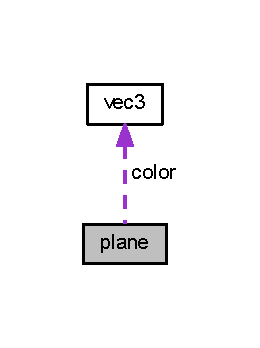
\includegraphics[width=125pt]{structplane__coll__graph}
\end{center}
\end{figure}
\subsection*{Data Fields}
\begin{DoxyCompactItemize}
\item 
\hyperlink{raymath_8h_aa97c1f529dc5a11a78758184c84a39c9}{number} \hyperlink{structplane_a0fef057ff8b9f6d358fcb427b1166edc}{axis}
\item 
\hyperlink{raymath_8h_aa97c1f529dc5a11a78758184c84a39c9}{number} \hyperlink{structplane_a07e9dd77b166f64838cd72a6213894ef}{dist}
\item 
\hyperlink{raymath_8h_afb3684d7701a8417d1a52fd94c84457c}{vec3\+\_\+t} \hyperlink{structplane_af1ec6dab64553dc67dc77bdc13deecb8}{color}
\end{DoxyCompactItemize}


\subsection{Detailed Description}


Definition at line 24 of file rayplane.\+h.



\subsection{Field Documentation}
\index{plane@{plane}!axis@{axis}}
\index{axis@{axis}!plane@{plane}}
\subsubsection[{\texorpdfstring{axis}{axis}}]{\setlength{\rightskip}{0pt plus 5cm}{\bf number} axis}\hypertarget{structplane_a0fef057ff8b9f6d358fcb427b1166edc}{}\label{structplane_a0fef057ff8b9f6d358fcb427b1166edc}
Plane axis (0 \+: x, 1 \+: y, 2 \+: z) 

Definition at line 25 of file rayplane.\+h.

\index{plane@{plane}!color@{color}}
\index{color@{color}!plane@{plane}}
\subsubsection[{\texorpdfstring{color}{color}}]{\setlength{\rightskip}{0pt plus 5cm}{\bf vec3\+\_\+t} color}\hypertarget{structplane_af1ec6dab64553dc67dc77bdc13deecb8}{}\label{structplane_af1ec6dab64553dc67dc77bdc13deecb8}
Plane color (rgb) 

Definition at line 27 of file rayplane.\+h.

\index{plane@{plane}!dist@{dist}}
\index{dist@{dist}!plane@{plane}}
\subsubsection[{\texorpdfstring{dist}{dist}}]{\setlength{\rightskip}{0pt plus 5cm}{\bf number} dist}\hypertarget{structplane_a07e9dd77b166f64838cd72a6213894ef}{}\label{structplane_a07e9dd77b166f64838cd72a6213894ef}
Plane distance to camera 

Definition at line 26 of file rayplane.\+h.



The documentation for this struct was generated from the following file\+:\begin{DoxyCompactItemize}
\item 
Includes/\hyperlink{rayplane_8h}{rayplane.\+h}\end{DoxyCompactItemize}

\hypertarget{structrayintersect}{}\section{rayintersect Struct Reference}
\label{structrayintersect}\index{rayintersect@{rayintersect}}


{\ttfamily \#include $<$rayintersect.\+h$>$}

\subsection*{Data Fields}
\begin{DoxyCompactItemize}
\item 
int \hyperlink{structrayintersect_ac765329451135abec74c45e1897abf26}{type}
\item 
int \hyperlink{structrayintersect_a750b5d744c39a06bfb13e6eb010e35d0}{index}
\item 
\hyperlink{raymath_8h_aa97c1f529dc5a11a78758184c84a39c9}{number} \hyperlink{structrayintersect_a07e9dd77b166f64838cd72a6213894ef}{dist}
\end{DoxyCompactItemize}


\subsection{Detailed Description}


Definition at line 24 of file rayintersect.\+h.



\subsection{Field Documentation}
\index{rayintersect@{rayintersect}!dist@{dist}}
\index{dist@{dist}!rayintersect@{rayintersect}}
\subsubsection[{\texorpdfstring{dist}{dist}}]{\setlength{\rightskip}{0pt plus 5cm}{\bf number} dist}\hypertarget{structrayintersect_a07e9dd77b166f64838cd72a6213894ef}{}\label{structrayintersect_a07e9dd77b166f64838cd72a6213894ef}
Distance from ray origin to intersection point 

Definition at line 27 of file rayintersect.\+h.

\index{rayintersect@{rayintersect}!index@{index}}
\index{index@{index}!rayintersect@{rayintersect}}
\subsubsection[{\texorpdfstring{index}{index}}]{\setlength{\rightskip}{0pt plus 5cm}int index}\hypertarget{structrayintersect_a750b5d744c39a06bfb13e6eb010e35d0}{}\label{structrayintersect_a750b5d744c39a06bfb13e6eb010e35d0}
Index of the object which has intersected with the ray 

Definition at line 26 of file rayintersect.\+h.

\index{rayintersect@{rayintersect}!type@{type}}
\index{type@{type}!rayintersect@{rayintersect}}
\subsubsection[{\texorpdfstring{type}{type}}]{\setlength{\rightskip}{0pt plus 5cm}int type}\hypertarget{structrayintersect_ac765329451135abec74c45e1897abf26}{}\label{structrayintersect_ac765329451135abec74c45e1897abf26}
Type of the object which has intersected with the ray 

Definition at line 25 of file rayintersect.\+h.



The documentation for this struct was generated from the following file\+:\begin{DoxyCompactItemize}
\item 
Includes/\hyperlink{rayintersect_8h}{rayintersect.\+h}\end{DoxyCompactItemize}

\hypertarget{structsphere}{}\section{sphere Struct Reference}
\label{structsphere}\index{sphere@{sphere}}


{\ttfamily \#include $<$raysphere.\+h$>$}



Collaboration diagram for sphere\+:\nopagebreak
\begin{figure}[H]
\begin{center}
\leavevmode
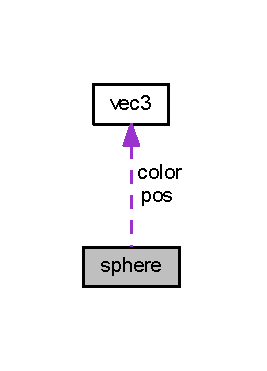
\includegraphics[width=128pt]{structsphere__coll__graph}
\end{center}
\end{figure}
\subsection*{Data Fields}
\begin{DoxyCompactItemize}
\item 
\hyperlink{raymath_8h_afb3684d7701a8417d1a52fd94c84457c}{vec3\+\_\+t} \hyperlink{structsphere_a81150a53dd49f693e71a6d68b213d99c}{pos}
\item 
\hyperlink{raymath_8h_aa97c1f529dc5a11a78758184c84a39c9}{number} \hyperlink{structsphere_a62fdcf65e893d786475a61de9f32f1e0}{r}
\item 
\hyperlink{raymath_8h_afb3684d7701a8417d1a52fd94c84457c}{vec3\+\_\+t} \hyperlink{structsphere_af1ec6dab64553dc67dc77bdc13deecb8}{color}
\item 
bool \hyperlink{structsphere_ac89a0bd6b5d17bfe81528537757ff5d8}{reflect}
\end{DoxyCompactItemize}


\subsection{Detailed Description}


Definition at line 24 of file raysphere.\+h.



\subsection{Field Documentation}
\index{sphere@{sphere}!color@{color}}
\index{color@{color}!sphere@{sphere}}
\subsubsection[{\texorpdfstring{color}{color}}]{\setlength{\rightskip}{0pt plus 5cm}{\bf vec3\+\_\+t} color}\hypertarget{structsphere_af1ec6dab64553dc67dc77bdc13deecb8}{}\label{structsphere_af1ec6dab64553dc67dc77bdc13deecb8}
Sphere color (rgb) 

Definition at line 27 of file raysphere.\+h.

\index{sphere@{sphere}!pos@{pos}}
\index{pos@{pos}!sphere@{sphere}}
\subsubsection[{\texorpdfstring{pos}{pos}}]{\setlength{\rightskip}{0pt plus 5cm}{\bf vec3\+\_\+t} pos}\hypertarget{structsphere_a81150a53dd49f693e71a6d68b213d99c}{}\label{structsphere_a81150a53dd49f693e71a6d68b213d99c}
Sphere position (xyz) 

Definition at line 25 of file raysphere.\+h.

\index{sphere@{sphere}!r@{r}}
\index{r@{r}!sphere@{sphere}}
\subsubsection[{\texorpdfstring{r}{r}}]{\setlength{\rightskip}{0pt plus 5cm}{\bf number} r}\hypertarget{structsphere_a62fdcf65e893d786475a61de9f32f1e0}{}\label{structsphere_a62fdcf65e893d786475a61de9f32f1e0}
Sphere radius 

Definition at line 26 of file raysphere.\+h.

\index{sphere@{sphere}!reflect@{reflect}}
\index{reflect@{reflect}!sphere@{sphere}}
\subsubsection[{\texorpdfstring{reflect}{reflect}}]{\setlength{\rightskip}{0pt plus 5cm}bool reflect}\hypertarget{structsphere_ac89a0bd6b5d17bfe81528537757ff5d8}{}\label{structsphere_ac89a0bd6b5d17bfe81528537757ff5d8}
Sphere reflection (false\+: disable reflection, true\+: enable reflection) 

Definition at line 28 of file raysphere.\+h.



The documentation for this struct was generated from the following file\+:\begin{DoxyCompactItemize}
\item 
Includes/\hyperlink{raysphere_8h}{raysphere.\+h}\end{DoxyCompactItemize}

\hypertarget{structvec3}{}\section{vec3 Struct Reference}
\label{structvec3}\index{vec3@{vec3}}


{\ttfamily \#include $<$raymath.\+h$>$}

\subsection*{Data Fields}
\begin{DoxyCompactItemize}
\item 
\hyperlink{raymath_8h_aa97c1f529dc5a11a78758184c84a39c9}{number} \hyperlink{structvec3_a117e8fdc0c12b911e0b4d7cf0e99c897}{x}
\item 
\hyperlink{raymath_8h_aa97c1f529dc5a11a78758184c84a39c9}{number} \hyperlink{structvec3_ae14c17bdf80bbde4381c61ddf63a7d98}{y}
\item 
\hyperlink{raymath_8h_aa97c1f529dc5a11a78758184c84a39c9}{number} \hyperlink{structvec3_ae59474797d4b0b7d7544bde5c6421230}{z}
\end{DoxyCompactItemize}


\subsection{Detailed Description}


Definition at line 82 of file raymath.\+h.



\subsection{Field Documentation}
\index{vec3@{vec3}!x@{x}}
\index{x@{x}!vec3@{vec3}}
\subsubsection[{\texorpdfstring{x}{x}}]{\setlength{\rightskip}{0pt plus 5cm}{\bf number} x}\hypertarget{structvec3_a117e8fdc0c12b911e0b4d7cf0e99c897}{}\label{structvec3_a117e8fdc0c12b911e0b4d7cf0e99c897}
x component 

Definition at line 83 of file raymath.\+h.

\index{vec3@{vec3}!y@{y}}
\index{y@{y}!vec3@{vec3}}
\subsubsection[{\texorpdfstring{y}{y}}]{\setlength{\rightskip}{0pt plus 5cm}{\bf number} y}\hypertarget{structvec3_ae14c17bdf80bbde4381c61ddf63a7d98}{}\label{structvec3_ae14c17bdf80bbde4381c61ddf63a7d98}
y component 

Definition at line 84 of file raymath.\+h.

\index{vec3@{vec3}!z@{z}}
\index{z@{z}!vec3@{vec3}}
\subsubsection[{\texorpdfstring{z}{z}}]{\setlength{\rightskip}{0pt plus 5cm}{\bf number} z}\hypertarget{structvec3_ae59474797d4b0b7d7544bde5c6421230}{}\label{structvec3_ae59474797d4b0b7d7544bde5c6421230}
z component 

Definition at line 85 of file raymath.\+h.



The documentation for this struct was generated from the following file\+:\begin{DoxyCompactItemize}
\item 
Includes/\hyperlink{raymath_8h}{raymath.\+h}\end{DoxyCompactItemize}

\chapter{File Documentation}
\hypertarget{rayintersect_8h}{}\section{Includes/rayintersect.h File Reference}
\label{rayintersect_8h}\index{Includes/rayintersect.\+h@{Includes/rayintersect.\+h}}


Raytracer ray intersection.  


{\ttfamily \#include $<$stdbool.\+h$>$}\\*
{\ttfamily \#include \char`\"{}raymath.\+h\char`\"{}}\\*
{\ttfamily \#include \char`\"{}raymathfix.\+h\char`\"{}}\\*
{\ttfamily \#include \char`\"{}rayplane.\+h\char`\"{}}\\*
{\ttfamily \#include \char`\"{}raysphere.\+h\char`\"{}}\\*
{\ttfamily \#include \char`\"{}rayobject.\+h\char`\"{}}\\*
Include dependency graph for rayintersect.\+h\+:\nopagebreak
\begin{figure}[H]
\begin{center}
\leavevmode
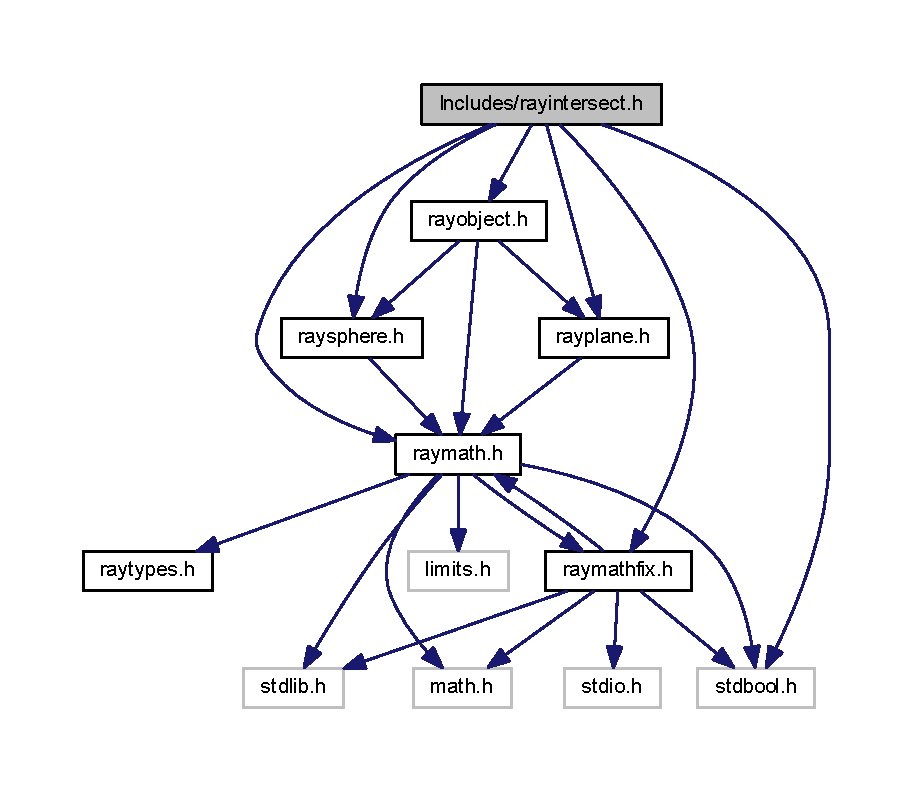
\includegraphics[width=350pt]{rayintersect_8h__incl}
\end{center}
\end{figure}
This graph shows which files directly or indirectly include this file\+:
\nopagebreak
\begin{figure}[H]
\begin{center}
\leavevmode
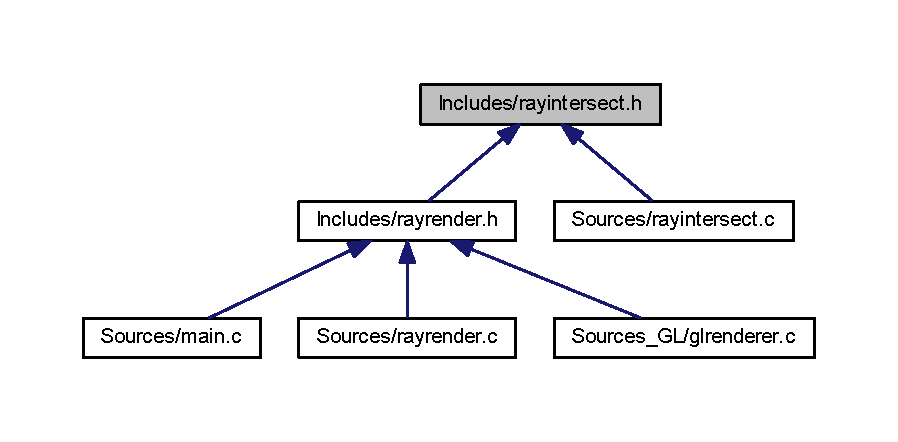
\includegraphics[width=350pt]{rayintersect_8h__dep__incl}
\end{center}
\end{figure}
\subsection*{Data Structures}
\begin{DoxyCompactItemize}
\item 
struct \hyperlink{structrayintersect}{rayintersect}
\end{DoxyCompactItemize}
\subsection*{Typedefs}
\begin{DoxyCompactItemize}
\item 
typedef struct \hyperlink{structrayintersect}{rayintersect} \hyperlink{rayintersect_8h_ad703c2567e842b299a9e6569790d090a}{rayintersect\+\_\+t}
\end{DoxyCompactItemize}
\subsection*{Functions}
\begin{DoxyCompactItemize}
\item 
bool \hyperlink{rayintersect_8h_a1e360dcbfb3c2b89c18fb0f1dc03a084}{Intersection\+Ray\+Object} (int type, int idx, \hyperlink{raymath_8h_afb3684d7701a8417d1a52fd94c84457c}{vec3\+\_\+t} r, \hyperlink{raymath_8h_afb3684d7701a8417d1a52fd94c84457c}{vec3\+\_\+t} o, \hyperlink{rayintersect_8h_ad703c2567e842b299a9e6569790d090a}{rayintersect\+\_\+t} $\ast$info)
\begin{DoxyCompactList}\small\item\em Test if an intersection between a ray and a object occurs. \end{DoxyCompactList}\end{DoxyCompactItemize}


\subsection{Detailed Description}
Raytracer ray intersection. 

\begin{DoxyAuthor}{Author}
J. Crenne \& C. Leroux 
\end{DoxyAuthor}
\begin{DoxyVersion}{Version}
1.\+0 
\end{DoxyVersion}
\begin{DoxyDate}{Date}
February 2016 
\end{DoxyDate}


\subsection{Typedef Documentation}
\index{rayintersect.\+h@{rayintersect.\+h}!rayintersect\+\_\+t@{rayintersect\+\_\+t}}
\index{rayintersect\+\_\+t@{rayintersect\+\_\+t}!rayintersect.\+h@{rayintersect.\+h}}
\subsubsection[{\texorpdfstring{rayintersect\+\_\+t}{rayintersect_t}}]{\setlength{\rightskip}{0pt plus 5cm}typedef struct {\bf rayintersect}  {\bf rayintersect\+\_\+t}}\hypertarget{rayintersect_8h_ad703c2567e842b299a9e6569790d090a}{}\label{rayintersect_8h_ad703c2567e842b299a9e6569790d090a}


\subsection{Function Documentation}
\index{rayintersect.\+h@{rayintersect.\+h}!Intersection\+Ray\+Object@{Intersection\+Ray\+Object}}
\index{Intersection\+Ray\+Object@{Intersection\+Ray\+Object}!rayintersect.\+h@{rayintersect.\+h}}
\subsubsection[{\texorpdfstring{Intersection\+Ray\+Object(int type, int idx, vec3\+\_\+t r, vec3\+\_\+t o, rayintersect\+\_\+t $\ast$info)}{IntersectionRayObject(int type, int idx, vec3_t r, vec3_t o, rayintersect_t *info)}}]{\setlength{\rightskip}{0pt plus 5cm}bool Intersection\+Ray\+Object (
\begin{DoxyParamCaption}
\item[{int}]{type, }
\item[{int}]{idx, }
\item[{{\bf vec3\+\_\+t}}]{r, }
\item[{{\bf vec3\+\_\+t}}]{o, }
\item[{{\bf rayintersect\+\_\+t} $\ast$}]{info}
\end{DoxyParamCaption}
)}\hypertarget{rayintersect_8h_a1e360dcbfb3c2b89c18fb0f1dc03a084}{}\label{rayintersect_8h_a1e360dcbfb3c2b89c18fb0f1dc03a084}


Test if an intersection between a ray and a object occurs. 


\begin{DoxyParams}{Parameters}
{\em type} & Object type ( O\+B\+J\+E\+C\+T\+\_\+\+T\+Y\+P\+E\+\_\+\+S\+P\+H\+E\+RE or O\+B\+J\+E\+C\+T\+\_\+\+T\+Y\+P\+E\+\_\+\+P\+L\+A\+NE ) \\
\hline
{\em idx} & Object identifier \\
\hline
{\em r} & Ray direction \\
\hline
{\em o} & Ray origin \\
\hline
{\em info} & A pointer holding a structure of intersection data \\
\hline
\end{DoxyParams}
\begin{DoxyReturn}{Returns}
True if an intersection occurs, false otherwise 
\end{DoxyReturn}


Definition at line 59 of file rayintersect.\+c.



Here is the caller graph for this function\+:\nopagebreak
\begin{figure}[H]
\begin{center}
\leavevmode
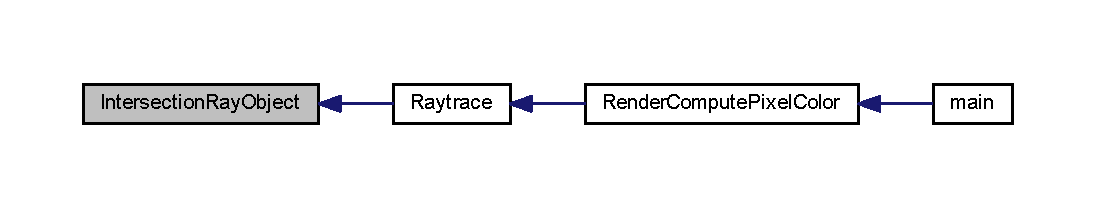
\includegraphics[width=350pt]{rayintersect_8h_a1e360dcbfb3c2b89c18fb0f1dc03a084_icgraph}
\end{center}
\end{figure}



\hypertarget{raylight_8h}{}\section{Includes/raylight.h File Reference}
\label{raylight_8h}\index{Includes/raylight.\+h@{Includes/raylight.\+h}}


Raytracer light.  


{\ttfamily \#include \char`\"{}raymath.\+h\char`\"{}}\\*
{\ttfamily \#include \char`\"{}rayobject.\+h\char`\"{}}\\*
Include dependency graph for raylight.\+h\+:\nopagebreak
\begin{figure}[H]
\begin{center}
\leavevmode
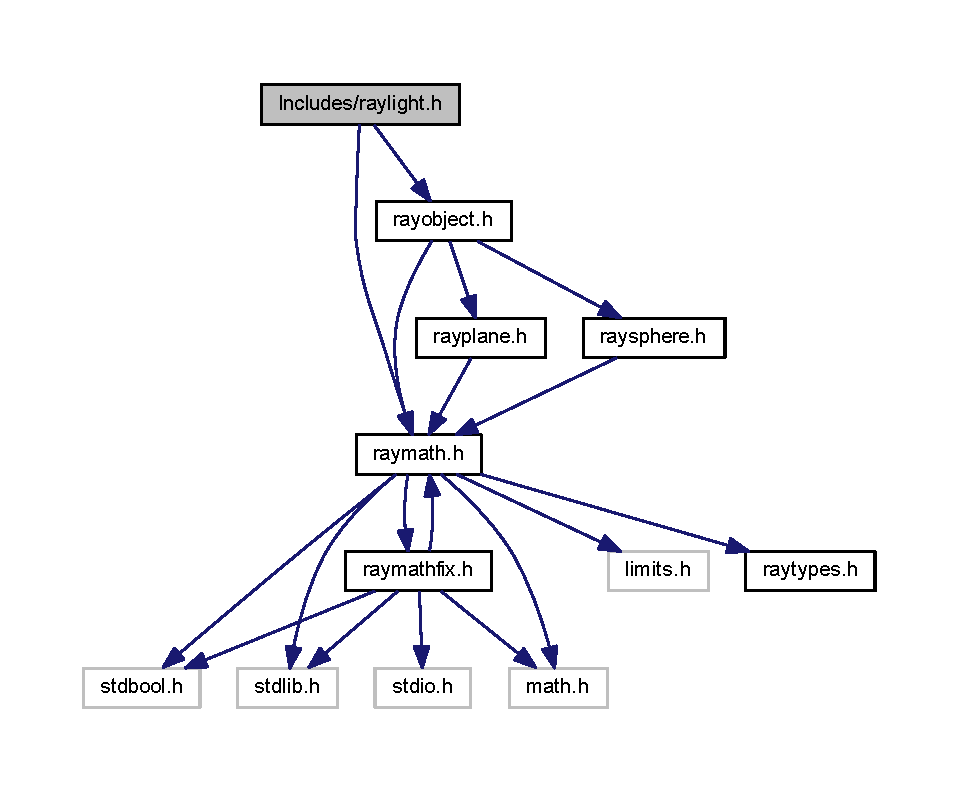
\includegraphics[width=350pt]{raylight_8h__incl}
\end{center}
\end{figure}
This graph shows which files directly or indirectly include this file\+:
\nopagebreak
\begin{figure}[H]
\begin{center}
\leavevmode
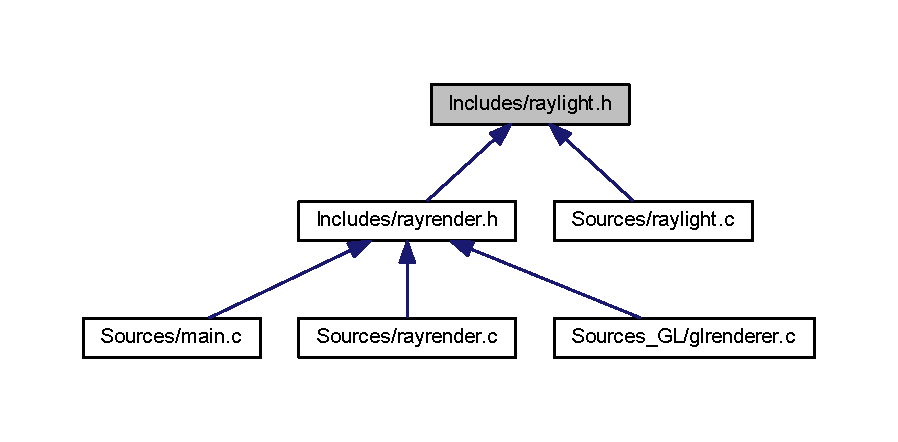
\includegraphics[width=350pt]{raylight_8h__dep__incl}
\end{center}
\end{figure}
\subsection*{Functions}
\begin{DoxyCompactItemize}
\item 
\hyperlink{raymath_8h_aa97c1f529dc5a11a78758184c84a39c9}{number} \hyperlink{raylight_8h_a233268c67064dbaf7faecaa4397ae31b}{Light\+Object} (int type, int idx, \hyperlink{raymath_8h_afb3684d7701a8417d1a52fd94c84457c}{vec3\+\_\+t} l, \hyperlink{raymath_8h_afb3684d7701a8417d1a52fd94c84457c}{vec3\+\_\+t} p, \hyperlink{raymath_8h_aa97c1f529dc5a11a78758184c84a39c9}{number} light\+Ambient)
\begin{DoxyCompactList}\small\item\em Get light contribution. \end{DoxyCompactList}\end{DoxyCompactItemize}


\subsection{Detailed Description}
Raytracer light. 

\begin{DoxyAuthor}{Author}
J. Crenne \& C. Leroux 
\end{DoxyAuthor}
\begin{DoxyVersion}{Version}
1.\+0 
\end{DoxyVersion}
\begin{DoxyDate}{Date}
February 2016 
\end{DoxyDate}


\subsection{Function Documentation}
\index{raylight.\+h@{raylight.\+h}!Light\+Object@{Light\+Object}}
\index{Light\+Object@{Light\+Object}!raylight.\+h@{raylight.\+h}}
\subsubsection[{\texorpdfstring{Light\+Object(int type, int idx, vec3\+\_\+t l, vec3\+\_\+t p, number light\+Ambient)}{LightObject(int type, int idx, vec3_t l, vec3_t p, number lightAmbient)}}]{\setlength{\rightskip}{0pt plus 5cm}{\bf number} Light\+Object (
\begin{DoxyParamCaption}
\item[{int}]{type, }
\item[{int}]{idx, }
\item[{{\bf vec3\+\_\+t}}]{l, }
\item[{{\bf vec3\+\_\+t}}]{p, }
\item[{{\bf number}}]{light\+Ambient}
\end{DoxyParamCaption}
)}\hypertarget{raylight_8h_a233268c67064dbaf7faecaa4397ae31b}{}\label{raylight_8h_a233268c67064dbaf7faecaa4397ae31b}


Get light contribution. 


\begin{DoxyParams}{Parameters}
{\em type} & Object type ( O\+B\+J\+E\+C\+T\+\_\+\+T\+Y\+P\+E\+\_\+\+S\+P\+H\+E\+RE or O\+B\+J\+E\+C\+T\+\_\+\+T\+Y\+P\+E\+\_\+\+P\+L\+A\+NE ) \\
\hline
{\em idx} & Object identifier \\
\hline
{\em l} & Light position \\
\hline
{\em p} & Intersection point position \\
\hline
{\em light\+Ambient} & Ambient light multiplier \\
\hline
\end{DoxyParams}
\begin{DoxyReturn}{Returns}
Light contribution to object 
\end{DoxyReturn}


Definition at line 16 of file raylight.\+c.



Here is the call graph for this function\+:\nopagebreak
\begin{figure}[H]
\begin{center}
\leavevmode
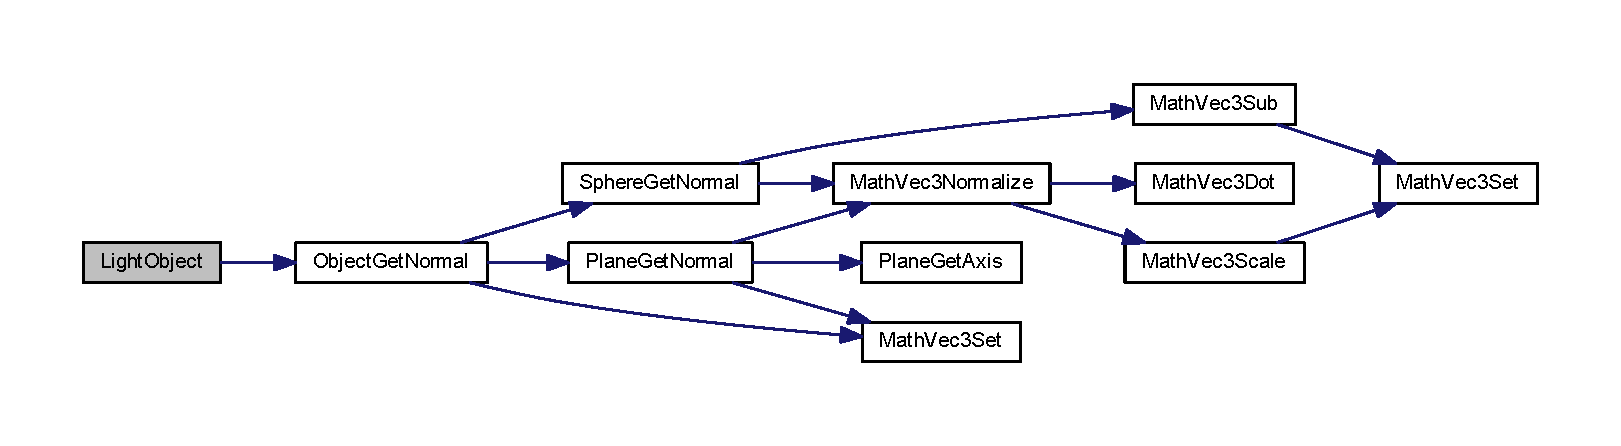
\includegraphics[width=350pt]{raylight_8h_a233268c67064dbaf7faecaa4397ae31b_cgraph}
\end{center}
\end{figure}




Here is the caller graph for this function\+:\nopagebreak
\begin{figure}[H]
\begin{center}
\leavevmode
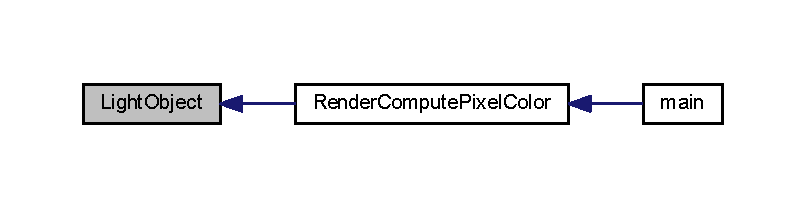
\includegraphics[width=350pt]{raylight_8h_a233268c67064dbaf7faecaa4397ae31b_icgraph}
\end{center}
\end{figure}



\hypertarget{raymath_8h}{}\section{Includes/raymath.h File Reference}
\label{raymath_8h}\index{Includes/raymath.\+h@{Includes/raymath.\+h}}


Raytracer math.  


{\ttfamily \#include $<$stdbool.\+h$>$}\\*
{\ttfamily \#include $<$stdlib.\+h$>$}\\*
{\ttfamily \#include $<$math.\+h$>$}\\*
{\ttfamily \#include $<$limits.\+h$>$}\\*
{\ttfamily \#include \char`\"{}raytypes.\+h\char`\"{}}\\*
{\ttfamily \#include \char`\"{}raymathfix.\+h\char`\"{}}\\*
Include dependency graph for raymath.\+h\+:\nopagebreak
\begin{figure}[H]
\begin{center}
\leavevmode
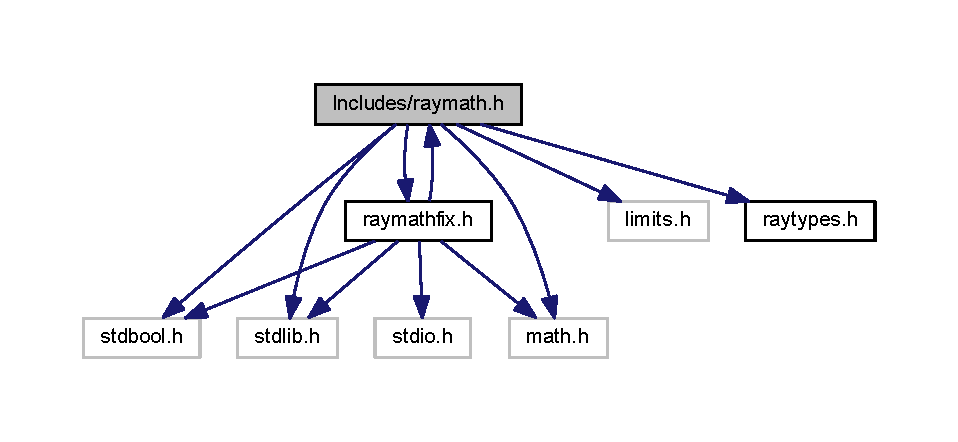
\includegraphics[width=350pt]{raymath_8h__incl}
\end{center}
\end{figure}
This graph shows which files directly or indirectly include this file\+:
\nopagebreak
\begin{figure}[H]
\begin{center}
\leavevmode
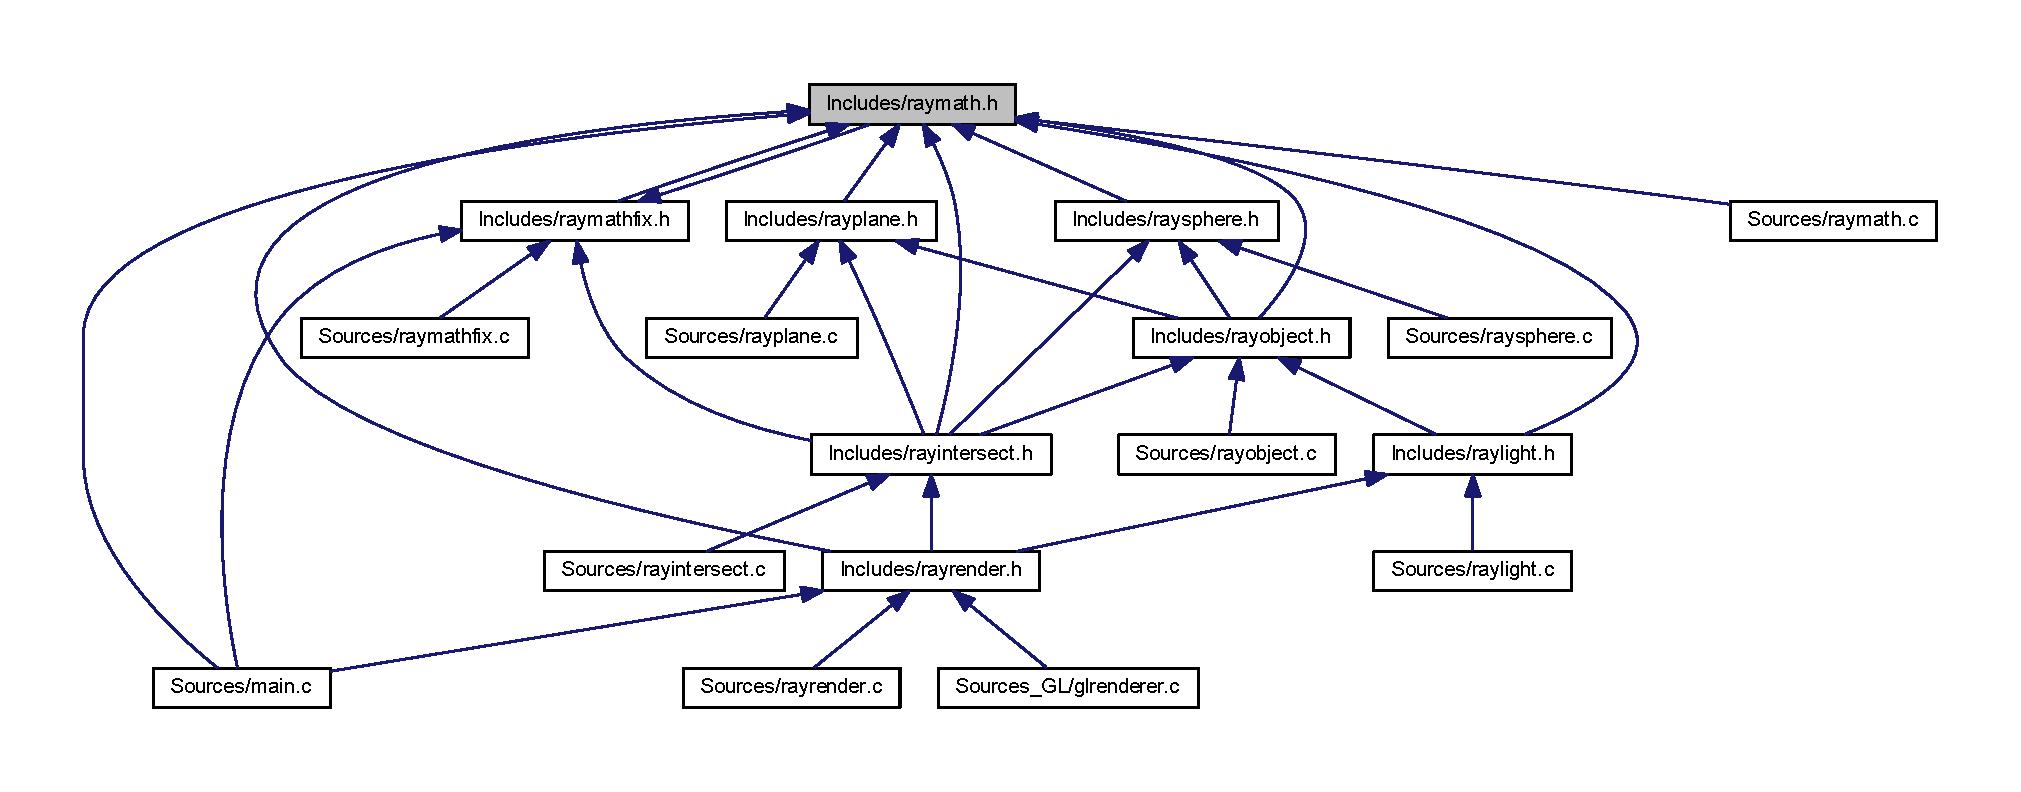
\includegraphics[width=350pt]{raymath_8h__dep__incl}
\end{center}
\end{figure}
\subsection*{Data Structures}
\begin{DoxyCompactItemize}
\item 
struct \hyperlink{structvec3}{vec3}
\end{DoxyCompactItemize}
\subsection*{Macros}
\begin{DoxyCompactItemize}
\item 
\#define \hyperlink{raymath_8h_a239c6887425f7b28cd09f280d1070850}{F\+I\+X\+\_\+\+I\+MP}
\begin{DoxyCompactList}\small\item\em Enable 32-\/bit fixed point raytracer implementation. \end{DoxyCompactList}\item 
\#define \hyperlink{raymath_8h_ad612104cac2f0a71d39241cdab09a8db}{Math\+Max}(a,  b)    ~(((a) $>$ (b)) ? (a) \+: (b))
\begin{DoxyCompactList}\small\item\em Get the maximum of two numbers. \end{DoxyCompactList}\item 
\#define \hyperlink{raymath_8h_ae2b0e98ddd7c8b1ff8a366eec892d027}{Math\+Min}(a,  b)    ~(((a) $<$ (b)) ? (a) \+: (b))
\begin{DoxyCompactList}\small\item\em Get the minimum of two numbers. \end{DoxyCompactList}\item 
\#define \hyperlink{raymath_8h_aa97c1f529dc5a11a78758184c84a39c9}{number}~\hyperlink{raytypes_8h_abab37cf41841dab8dc81b8da87acd6c5}{fixed}
\item 
\#define \hyperlink{raymath_8h_a5f35899b3b66a3a746eef56145fd831f}{T}(f)~\hyperlink{raymathfix_8h_ab5cadba2a8639b9ef54ab46b3155799c}{Math\+Float2\+Fix}( f )
\item 
\#define \hyperlink{raymath_8h_a1a14019f88db2a0b038688cd9830ea7e}{add}(a,  b)~\hyperlink{raymathfix_8h_a662a769f40ac43a3d5e1afeda0f0e9c9}{Math\+Fix\+Add}( a, b )
\item 
\#define \hyperlink{raymath_8h_abc9bcff6c9dcede2fb7ec8e2ddff3358}{sub}(a,  b)~\hyperlink{raymathfix_8h_a9efdd30e8c235b4e7d710adfa2b933dc}{Math\+Fix\+Sub}( a, b )
\item 
\#define \hyperlink{raymath_8h_a0da29b54f1662523e9e9da60dde8b629}{mul}(a,  b)~\hyperlink{raymathfix_8h_a8d93126fdac6ca6825b80576bed9a7c5}{Math\+Fix\+Mul}( a, b )
\item 
\#define \hyperlink{raymath_8h_a5029d66da963c87e7314612c3102276a}{div}(a,  b)~\hyperlink{raymathfix_8h_a00f0fef6f042f8aea5ce731a68a3316a}{Math\+Fix\+Div}( a, b )
\item 
\#define \hyperlink{raymath_8h_a09f4b0d9da085264ffcb8d68fa045d67}{sqr}(a)~\hyperlink{raymathfix_8c_af55120a972b12f1773e0b5a95f92bea8}{Math\+Fix\+Sqrt}( a )
\item 
\#define \hyperlink{raymath_8h_aa2eab56fea61c2b43c875652a9115d5c}{E\+P\+S\+\_\+\+V\+A\+L\+UE}~1 $<$$<$ \hyperlink{raymathfix_8h_a8edc3240c157eecf1131299de27dea7a}{F\+I\+X\+\_\+\+S\+H\+I\+FT}
\item 
\#define \hyperlink{raymath_8h_a4ce3e2af80a76d816ab7f8567ec4a65a}{M\+A\+X\+\_\+\+V\+A\+L\+UE}~I\+N\+T\+\_\+\+M\+AX
\item 
\#define \hyperlink{raymath_8h_ac328e551bde3d39b6d7b8cc9e048d941}{Z\+E\+RO}~0
\end{DoxyCompactItemize}
\subsection*{Typedefs}
\begin{DoxyCompactItemize}
\item 
typedef struct \hyperlink{structvec3}{vec3} \hyperlink{raymath_8h_afb3684d7701a8417d1a52fd94c84457c}{vec3\+\_\+t}
\begin{DoxyCompactList}\small\item\em A Structure to represent a 3D vector. \end{DoxyCompactList}\end{DoxyCompactItemize}
\subsection*{Functions}
\begin{DoxyCompactItemize}
\item 
\hyperlink{raymath_8h_aa97c1f529dc5a11a78758184c84a39c9}{number} \hyperlink{raymath_8h_af55120a972b12f1773e0b5a95f92bea8}{Math\+Fix\+Sqrt} (\hyperlink{raymath_8h_aa97c1f529dc5a11a78758184c84a39c9}{number} n)
\begin{DoxyCompactList}\small\item\em Float implementation of square root of n. \end{DoxyCompactList}\item 
\hyperlink{raymath_8h_aa97c1f529dc5a11a78758184c84a39c9}{number} \hyperlink{raymath_8h_ad23db858056b973907f7dfc34cd430e5}{Math\+Clamp} (\hyperlink{raymath_8h_aa97c1f529dc5a11a78758184c84a39c9}{number} d, \hyperlink{raymath_8h_aa97c1f529dc5a11a78758184c84a39c9}{number} min, \hyperlink{raymath_8h_aa97c1f529dc5a11a78758184c84a39c9}{number} max)
\begin{DoxyCompactList}\small\item\em Clamp a number between a range. \end{DoxyCompactList}\item 
bool \hyperlink{raymath_8h_a4f748dcf42de8f0879bf0ff7ef9f4f36}{Math\+Is\+Odd} (int x)
\begin{DoxyCompactList}\small\item\em Get the parity of a integer. \end{DoxyCompactList}\item 
\hyperlink{raymath_8h_afb3684d7701a8417d1a52fd94c84457c}{vec3\+\_\+t} \hyperlink{raymath_8h_a0c3b96d5e78c8899245e367835c0e1b4}{Math\+Vec3\+Set} (\hyperlink{raymath_8h_aa97c1f529dc5a11a78758184c84a39c9}{number} x, \hyperlink{raymath_8h_aa97c1f529dc5a11a78758184c84a39c9}{number} y, \hyperlink{raymath_8h_aa97c1f529dc5a11a78758184c84a39c9}{number} z)
\begin{DoxyCompactList}\small\item\em Set a 3D vector. \end{DoxyCompactList}\item 
\hyperlink{raymath_8h_afb3684d7701a8417d1a52fd94c84457c}{vec3\+\_\+t} \hyperlink{raymath_8h_a1d9b3e20abf08441155772741c0ef939}{Math\+Vec3\+Add} (\hyperlink{raymath_8h_afb3684d7701a8417d1a52fd94c84457c}{vec3\+\_\+t} a, \hyperlink{raymath_8h_afb3684d7701a8417d1a52fd94c84457c}{vec3\+\_\+t} b)
\begin{DoxyCompactList}\small\item\em Add two 3D vectors. \end{DoxyCompactList}\item 
\hyperlink{raymath_8h_afb3684d7701a8417d1a52fd94c84457c}{vec3\+\_\+t} \hyperlink{raymath_8h_afc53ea0adde49d6b23d3d20f7242ce3b}{Math\+Vec3\+Sub} (\hyperlink{raymath_8h_afb3684d7701a8417d1a52fd94c84457c}{vec3\+\_\+t} a, \hyperlink{raymath_8h_afb3684d7701a8417d1a52fd94c84457c}{vec3\+\_\+t} b)
\begin{DoxyCompactList}\small\item\em Subtract two 3D vectors. \end{DoxyCompactList}\item 
\hyperlink{raymath_8h_aa97c1f529dc5a11a78758184c84a39c9}{number} \hyperlink{raymath_8h_aa67fbe59543039467aa720334738e2a2}{Math\+Vec3\+Dot} (\hyperlink{raymath_8h_afb3684d7701a8417d1a52fd94c84457c}{vec3\+\_\+t} a, \hyperlink{raymath_8h_afb3684d7701a8417d1a52fd94c84457c}{vec3\+\_\+t} b)
\begin{DoxyCompactList}\small\item\em Compute the dot product between two vectors. \end{DoxyCompactList}\item 
\hyperlink{raymath_8h_afb3684d7701a8417d1a52fd94c84457c}{vec3\+\_\+t} \hyperlink{raymath_8h_a414c0be0d1f209943c3ecbbae79002d2}{Math\+Vec3\+Scale} (\hyperlink{raymath_8h_afb3684d7701a8417d1a52fd94c84457c}{vec3\+\_\+t} a, \hyperlink{raymath_8h_aa97c1f529dc5a11a78758184c84a39c9}{number} c)
\begin{DoxyCompactList}\small\item\em Scale a 3D vector (multiply by a scalar) \end{DoxyCompactList}\item 
\hyperlink{raymath_8h_afb3684d7701a8417d1a52fd94c84457c}{vec3\+\_\+t} \hyperlink{raymath_8h_a075c2db2a273d9e2ab085f4cba6fbf9f}{Math\+Vec3\+Normalize} (\hyperlink{raymath_8h_afb3684d7701a8417d1a52fd94c84457c}{vec3\+\_\+t} v)
\begin{DoxyCompactList}\small\item\em Normalize a 3D vector. \end{DoxyCompactList}\end{DoxyCompactItemize}


\subsection{Detailed Description}
Raytracer math. 

\begin{DoxyAuthor}{Author}
J. Crenne \& C. Leroux 
\end{DoxyAuthor}
\begin{DoxyVersion}{Version}
1.\+0 
\end{DoxyVersion}
\begin{DoxyDate}{Date}
February 2016 
\end{DoxyDate}


\subsection{Macro Definition Documentation}
\index{raymath.\+h@{raymath.\+h}!add@{add}}
\index{add@{add}!raymath.\+h@{raymath.\+h}}
\subsubsection[{\texorpdfstring{add}{add}}]{\setlength{\rightskip}{0pt plus 5cm}\#define add(
\begin{DoxyParamCaption}
\item[{}]{a, }
\item[{}]{b}
\end{DoxyParamCaption}
)~{\bf Math\+Fix\+Add}( a, b )}\hypertarget{raymath_8h_a1a14019f88db2a0b038688cd9830ea7e}{}\label{raymath_8h_a1a14019f88db2a0b038688cd9830ea7e}


Definition at line 65 of file raymath.\+h.

\index{raymath.\+h@{raymath.\+h}!div@{div}}
\index{div@{div}!raymath.\+h@{raymath.\+h}}
\subsubsection[{\texorpdfstring{div}{div}}]{\setlength{\rightskip}{0pt plus 5cm}\#define div(
\begin{DoxyParamCaption}
\item[{}]{a, }
\item[{}]{b}
\end{DoxyParamCaption}
)~{\bf Math\+Fix\+Div}( a, b )}\hypertarget{raymath_8h_a5029d66da963c87e7314612c3102276a}{}\label{raymath_8h_a5029d66da963c87e7314612c3102276a}


Definition at line 68 of file raymath.\+h.

\index{raymath.\+h@{raymath.\+h}!E\+P\+S\+\_\+\+V\+A\+L\+UE@{E\+P\+S\+\_\+\+V\+A\+L\+UE}}
\index{E\+P\+S\+\_\+\+V\+A\+L\+UE@{E\+P\+S\+\_\+\+V\+A\+L\+UE}!raymath.\+h@{raymath.\+h}}
\subsubsection[{\texorpdfstring{E\+P\+S\+\_\+\+V\+A\+L\+UE}{EPS_VALUE}}]{\setlength{\rightskip}{0pt plus 5cm}\#define E\+P\+S\+\_\+\+V\+A\+L\+UE~1 $<$$<$ {\bf F\+I\+X\+\_\+\+S\+H\+I\+FT}}\hypertarget{raymath_8h_aa2eab56fea61c2b43c875652a9115d5c}{}\label{raymath_8h_aa2eab56fea61c2b43c875652a9115d5c}


Definition at line 71 of file raymath.\+h.

\index{raymath.\+h@{raymath.\+h}!F\+I\+X\+\_\+\+I\+MP@{F\+I\+X\+\_\+\+I\+MP}}
\index{F\+I\+X\+\_\+\+I\+MP@{F\+I\+X\+\_\+\+I\+MP}!raymath.\+h@{raymath.\+h}}
\subsubsection[{\texorpdfstring{F\+I\+X\+\_\+\+I\+MP}{FIX_IMP}}]{\setlength{\rightskip}{0pt plus 5cm}\#define F\+I\+X\+\_\+\+I\+MP}\hypertarget{raymath_8h_a239c6887425f7b28cd09f280d1070850}{}\label{raymath_8h_a239c6887425f7b28cd09f280d1070850}


Enable 32-\/bit fixed point raytracer implementation. 



Definition at line 24 of file raymath.\+h.

\index{raymath.\+h@{raymath.\+h}!Math\+Max@{Math\+Max}}
\index{Math\+Max@{Math\+Max}!raymath.\+h@{raymath.\+h}}
\subsubsection[{\texorpdfstring{Math\+Max}{MathMax}}]{\setlength{\rightskip}{0pt plus 5cm}\#define Math\+Max(
\begin{DoxyParamCaption}
\item[{}]{a, }
\item[{}]{b}
\end{DoxyParamCaption}
)~(((a) $>$ (b)) ? (a) \+: (b))}\hypertarget{raymath_8h_ad612104cac2f0a71d39241cdab09a8db}{}\label{raymath_8h_ad612104cac2f0a71d39241cdab09a8db}


Get the maximum of two numbers. 



Definition at line 36 of file raymath.\+h.

\index{raymath.\+h@{raymath.\+h}!Math\+Min@{Math\+Min}}
\index{Math\+Min@{Math\+Min}!raymath.\+h@{raymath.\+h}}
\subsubsection[{\texorpdfstring{Math\+Min}{MathMin}}]{\setlength{\rightskip}{0pt plus 5cm}\#define Math\+Min(
\begin{DoxyParamCaption}
\item[{}]{a, }
\item[{}]{b}
\end{DoxyParamCaption}
)~(((a) $<$ (b)) ? (a) \+: (b))}\hypertarget{raymath_8h_ae2b0e98ddd7c8b1ff8a366eec892d027}{}\label{raymath_8h_ae2b0e98ddd7c8b1ff8a366eec892d027}


Get the minimum of two numbers. 



Definition at line 42 of file raymath.\+h.

\index{raymath.\+h@{raymath.\+h}!M\+A\+X\+\_\+\+V\+A\+L\+UE@{M\+A\+X\+\_\+\+V\+A\+L\+UE}}
\index{M\+A\+X\+\_\+\+V\+A\+L\+UE@{M\+A\+X\+\_\+\+V\+A\+L\+UE}!raymath.\+h@{raymath.\+h}}
\subsubsection[{\texorpdfstring{M\+A\+X\+\_\+\+V\+A\+L\+UE}{MAX_VALUE}}]{\setlength{\rightskip}{0pt plus 5cm}\#define M\+A\+X\+\_\+\+V\+A\+L\+UE~I\+N\+T\+\_\+\+M\+AX}\hypertarget{raymath_8h_a4ce3e2af80a76d816ab7f8567ec4a65a}{}\label{raymath_8h_a4ce3e2af80a76d816ab7f8567ec4a65a}


Definition at line 72 of file raymath.\+h.

\index{raymath.\+h@{raymath.\+h}!mul@{mul}}
\index{mul@{mul}!raymath.\+h@{raymath.\+h}}
\subsubsection[{\texorpdfstring{mul}{mul}}]{\setlength{\rightskip}{0pt plus 5cm}\#define mul(
\begin{DoxyParamCaption}
\item[{}]{a, }
\item[{}]{b}
\end{DoxyParamCaption}
)~{\bf Math\+Fix\+Mul}( a, b )}\hypertarget{raymath_8h_a0da29b54f1662523e9e9da60dde8b629}{}\label{raymath_8h_a0da29b54f1662523e9e9da60dde8b629}


Definition at line 67 of file raymath.\+h.

\index{raymath.\+h@{raymath.\+h}!number@{number}}
\index{number@{number}!raymath.\+h@{raymath.\+h}}
\subsubsection[{\texorpdfstring{number}{number}}]{\setlength{\rightskip}{0pt plus 5cm}\#define number~{\bf fixed}}\hypertarget{raymath_8h_aa97c1f529dc5a11a78758184c84a39c9}{}\label{raymath_8h_aa97c1f529dc5a11a78758184c84a39c9}


Definition at line 62 of file raymath.\+h.

\index{raymath.\+h@{raymath.\+h}!sqr@{sqr}}
\index{sqr@{sqr}!raymath.\+h@{raymath.\+h}}
\subsubsection[{\texorpdfstring{sqr}{sqr}}]{\setlength{\rightskip}{0pt plus 5cm}\#define sqr(
\begin{DoxyParamCaption}
\item[{}]{a}
\end{DoxyParamCaption}
)~{\bf Math\+Fix\+Sqrt}( a )}\hypertarget{raymath_8h_a09f4b0d9da085264ffcb8d68fa045d67}{}\label{raymath_8h_a09f4b0d9da085264ffcb8d68fa045d67}


Definition at line 69 of file raymath.\+h.

\index{raymath.\+h@{raymath.\+h}!sub@{sub}}
\index{sub@{sub}!raymath.\+h@{raymath.\+h}}
\subsubsection[{\texorpdfstring{sub}{sub}}]{\setlength{\rightskip}{0pt plus 5cm}\#define sub(
\begin{DoxyParamCaption}
\item[{}]{a, }
\item[{}]{b}
\end{DoxyParamCaption}
)~{\bf Math\+Fix\+Sub}( a, b )}\hypertarget{raymath_8h_abc9bcff6c9dcede2fb7ec8e2ddff3358}{}\label{raymath_8h_abc9bcff6c9dcede2fb7ec8e2ddff3358}


Definition at line 66 of file raymath.\+h.

\index{raymath.\+h@{raymath.\+h}!T@{T}}
\index{T@{T}!raymath.\+h@{raymath.\+h}}
\subsubsection[{\texorpdfstring{T}{T}}]{\setlength{\rightskip}{0pt plus 5cm}\#define T(
\begin{DoxyParamCaption}
\item[{}]{f}
\end{DoxyParamCaption}
)~{\bf Math\+Float2\+Fix}( f )}\hypertarget{raymath_8h_a5f35899b3b66a3a746eef56145fd831f}{}\label{raymath_8h_a5f35899b3b66a3a746eef56145fd831f}


Definition at line 64 of file raymath.\+h.

\index{raymath.\+h@{raymath.\+h}!Z\+E\+RO@{Z\+E\+RO}}
\index{Z\+E\+RO@{Z\+E\+RO}!raymath.\+h@{raymath.\+h}}
\subsubsection[{\texorpdfstring{Z\+E\+RO}{ZERO}}]{\setlength{\rightskip}{0pt plus 5cm}\#define Z\+E\+RO~0}\hypertarget{raymath_8h_ac328e551bde3d39b6d7b8cc9e048d941}{}\label{raymath_8h_ac328e551bde3d39b6d7b8cc9e048d941}


Definition at line 73 of file raymath.\+h.



\subsection{Typedef Documentation}
\index{raymath.\+h@{raymath.\+h}!vec3\+\_\+t@{vec3\+\_\+t}}
\index{vec3\+\_\+t@{vec3\+\_\+t}!raymath.\+h@{raymath.\+h}}
\subsubsection[{\texorpdfstring{vec3\+\_\+t}{vec3_t}}]{\setlength{\rightskip}{0pt plus 5cm}{\bf vec3\+\_\+t}}\hypertarget{raymath_8h_afb3684d7701a8417d1a52fd94c84457c}{}\label{raymath_8h_afb3684d7701a8417d1a52fd94c84457c}


A Structure to represent a 3D vector. 



\subsection{Function Documentation}
\index{raymath.\+h@{raymath.\+h}!Math\+Clamp@{Math\+Clamp}}
\index{Math\+Clamp@{Math\+Clamp}!raymath.\+h@{raymath.\+h}}
\subsubsection[{\texorpdfstring{Math\+Clamp(number d, number min, number max)}{MathClamp(number d, number min, number max)}}]{\setlength{\rightskip}{0pt plus 5cm}{\bf number} Math\+Clamp (
\begin{DoxyParamCaption}
\item[{{\bf number}}]{d, }
\item[{{\bf number}}]{min, }
\item[{{\bf number}}]{max}
\end{DoxyParamCaption}
)}\hypertarget{raymath_8h_ad23db858056b973907f7dfc34cd430e5}{}\label{raymath_8h_ad23db858056b973907f7dfc34cd430e5}


Clamp a number between a range. 


\begin{DoxyParams}{Parameters}
{\em d} & number to clamp \\
\hline
{\em min} & minimum number range \\
\hline
{\em max} & maximum number range \\
\hline
\end{DoxyParams}
\begin{DoxyReturn}{Returns}
clamped number 
\end{DoxyReturn}


Definition at line 12 of file raymath.\+c.

\index{raymath.\+h@{raymath.\+h}!Math\+Fix\+Sqrt@{Math\+Fix\+Sqrt}}
\index{Math\+Fix\+Sqrt@{Math\+Fix\+Sqrt}!raymath.\+h@{raymath.\+h}}
\subsubsection[{\texorpdfstring{Math\+Fix\+Sqrt(number n)}{MathFixSqrt(number n)}}]{\setlength{\rightskip}{0pt plus 5cm}{\bf number} Math\+Fix\+Sqrt (
\begin{DoxyParamCaption}
\item[{{\bf number}}]{n}
\end{DoxyParamCaption}
)}\hypertarget{raymath_8h_af55120a972b12f1773e0b5a95f92bea8}{}\label{raymath_8h_af55120a972b12f1773e0b5a95f92bea8}


Float implementation of square root of n. 

Fixed implementation of square root of n 

Definition at line 29 of file raymathfix.\+c.

\index{raymath.\+h@{raymath.\+h}!Math\+Is\+Odd@{Math\+Is\+Odd}}
\index{Math\+Is\+Odd@{Math\+Is\+Odd}!raymath.\+h@{raymath.\+h}}
\subsubsection[{\texorpdfstring{Math\+Is\+Odd(int x)}{MathIsOdd(int x)}}]{\setlength{\rightskip}{0pt plus 5cm}bool Math\+Is\+Odd (
\begin{DoxyParamCaption}
\item[{int}]{x}
\end{DoxyParamCaption}
)}\hypertarget{raymath_8h_a4f748dcf42de8f0879bf0ff7ef9f4f36}{}\label{raymath_8h_a4f748dcf42de8f0879bf0ff7ef9f4f36}


Get the parity of a integer. 


\begin{DoxyParams}{Parameters}
{\em x} & integer to test \\
\hline
\end{DoxyParams}
\begin{DoxyReturn}{Returns}
true if the integer is odd, false if even 
\end{DoxyReturn}


Definition at line 17 of file raymath.\+c.

\index{raymath.\+h@{raymath.\+h}!Math\+Vec3\+Add@{Math\+Vec3\+Add}}
\index{Math\+Vec3\+Add@{Math\+Vec3\+Add}!raymath.\+h@{raymath.\+h}}
\subsubsection[{\texorpdfstring{Math\+Vec3\+Add(vec3\+\_\+t a, vec3\+\_\+t b)}{MathVec3Add(vec3_t a, vec3_t b)}}]{\setlength{\rightskip}{0pt plus 5cm}{\bf vec3\+\_\+t} Math\+Vec3\+Add (
\begin{DoxyParamCaption}
\item[{{\bf vec3\+\_\+t}}]{a, }
\item[{{\bf vec3\+\_\+t}}]{b}
\end{DoxyParamCaption}
)}\hypertarget{raymath_8h_a1d9b3e20abf08441155772741c0ef939}{}\label{raymath_8h_a1d9b3e20abf08441155772741c0ef939}


Add two 3D vectors. 


\begin{DoxyParams}{Parameters}
{\em a} & 3D vector \\
\hline
{\em b} & 3D vector \\
\hline
\end{DoxyParams}
\begin{DoxyReturn}{Returns}
resulting 3D vector (a + b) 
\end{DoxyReturn}


Definition at line 29 of file raymath.\+c.



Here is the call graph for this function\+:\nopagebreak
\begin{figure}[H]
\begin{center}
\leavevmode
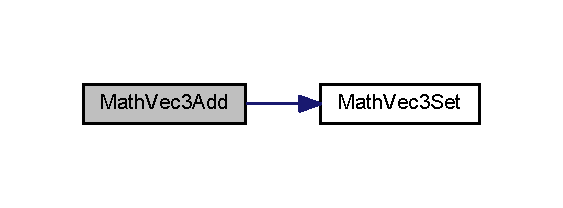
\includegraphics[width=270pt]{raymath_8h_a1d9b3e20abf08441155772741c0ef939_cgraph}
\end{center}
\end{figure}




Here is the caller graph for this function\+:\nopagebreak
\begin{figure}[H]
\begin{center}
\leavevmode
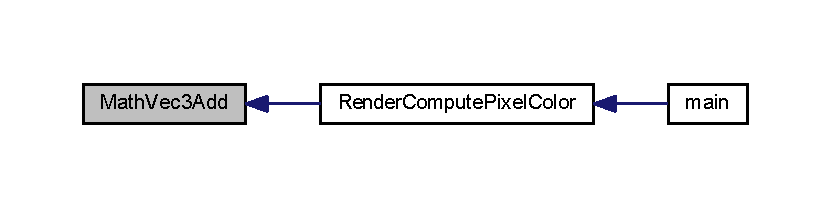
\includegraphics[width=350pt]{raymath_8h_a1d9b3e20abf08441155772741c0ef939_icgraph}
\end{center}
\end{figure}


\index{raymath.\+h@{raymath.\+h}!Math\+Vec3\+Dot@{Math\+Vec3\+Dot}}
\index{Math\+Vec3\+Dot@{Math\+Vec3\+Dot}!raymath.\+h@{raymath.\+h}}
\subsubsection[{\texorpdfstring{Math\+Vec3\+Dot(vec3\+\_\+t a, vec3\+\_\+t b)}{MathVec3Dot(vec3_t a, vec3_t b)}}]{\setlength{\rightskip}{0pt plus 5cm}{\bf number} Math\+Vec3\+Dot (
\begin{DoxyParamCaption}
\item[{{\bf vec3\+\_\+t}}]{a, }
\item[{{\bf vec3\+\_\+t}}]{b}
\end{DoxyParamCaption}
)}\hypertarget{raymath_8h_aa67fbe59543039467aa720334738e2a2}{}\label{raymath_8h_aa67fbe59543039467aa720334738e2a2}


Compute the dot product between two vectors. 


\begin{DoxyParams}{Parameters}
{\em a} & 3D vector \\
\hline
{\em b} & 3D vector \\
\hline
\end{DoxyParams}
\begin{DoxyReturn}{Returns}
resulting dot product (a . b) 
\end{DoxyReturn}


Definition at line 44 of file raymath.\+c.



Here is the caller graph for this function\+:\nopagebreak
\begin{figure}[H]
\begin{center}
\leavevmode
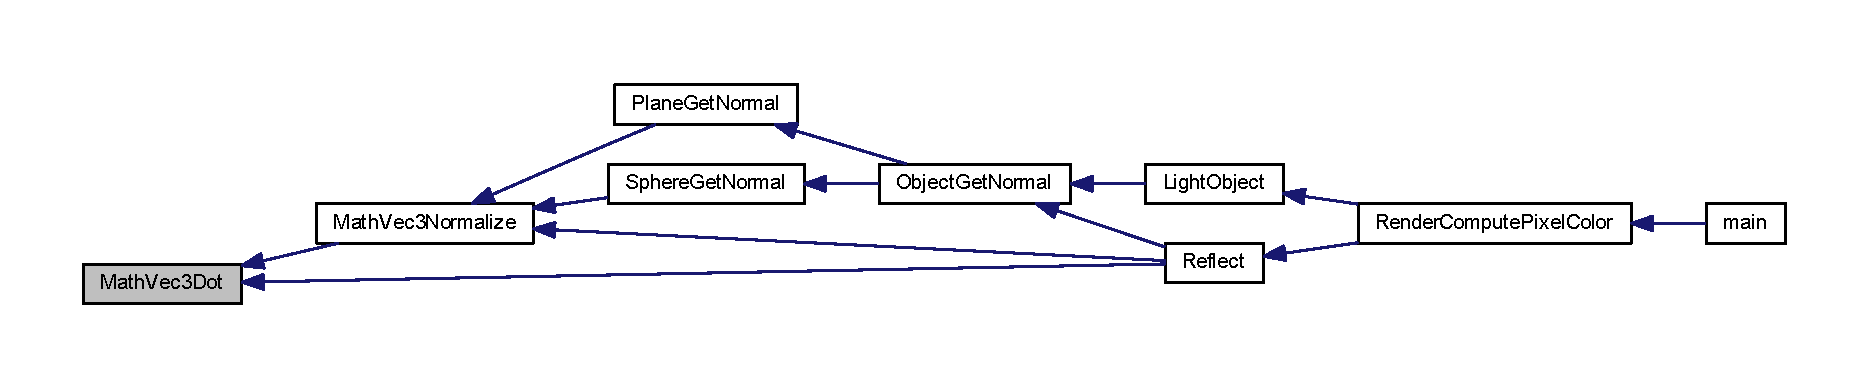
\includegraphics[width=350pt]{raymath_8h_aa67fbe59543039467aa720334738e2a2_icgraph}
\end{center}
\end{figure}


\index{raymath.\+h@{raymath.\+h}!Math\+Vec3\+Normalize@{Math\+Vec3\+Normalize}}
\index{Math\+Vec3\+Normalize@{Math\+Vec3\+Normalize}!raymath.\+h@{raymath.\+h}}
\subsubsection[{\texorpdfstring{Math\+Vec3\+Normalize(vec3\+\_\+t v)}{MathVec3Normalize(vec3_t v)}}]{\setlength{\rightskip}{0pt plus 5cm}{\bf vec3\+\_\+t} Math\+Vec3\+Normalize (
\begin{DoxyParamCaption}
\item[{{\bf vec3\+\_\+t}}]{v}
\end{DoxyParamCaption}
)}\hypertarget{raymath_8h_a075c2db2a273d9e2ab085f4cba6fbf9f}{}\label{raymath_8h_a075c2db2a273d9e2ab085f4cba6fbf9f}


Normalize a 3D vector. 


\begin{DoxyParams}{Parameters}
{\em v} & 3D vector \\
\hline
\end{DoxyParams}
\begin{DoxyReturn}{Returns}
normalized 3D vector 
\end{DoxyReturn}


Definition at line 52 of file raymath.\+c.



Here is the call graph for this function\+:\nopagebreak
\begin{figure}[H]
\begin{center}
\leavevmode
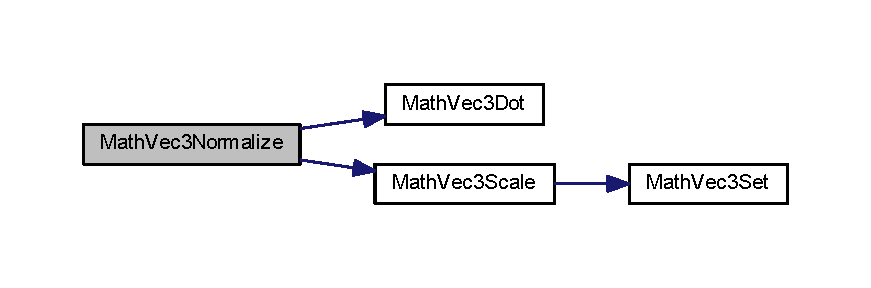
\includegraphics[width=350pt]{raymath_8h_a075c2db2a273d9e2ab085f4cba6fbf9f_cgraph}
\end{center}
\end{figure}




Here is the caller graph for this function\+:\nopagebreak
\begin{figure}[H]
\begin{center}
\leavevmode
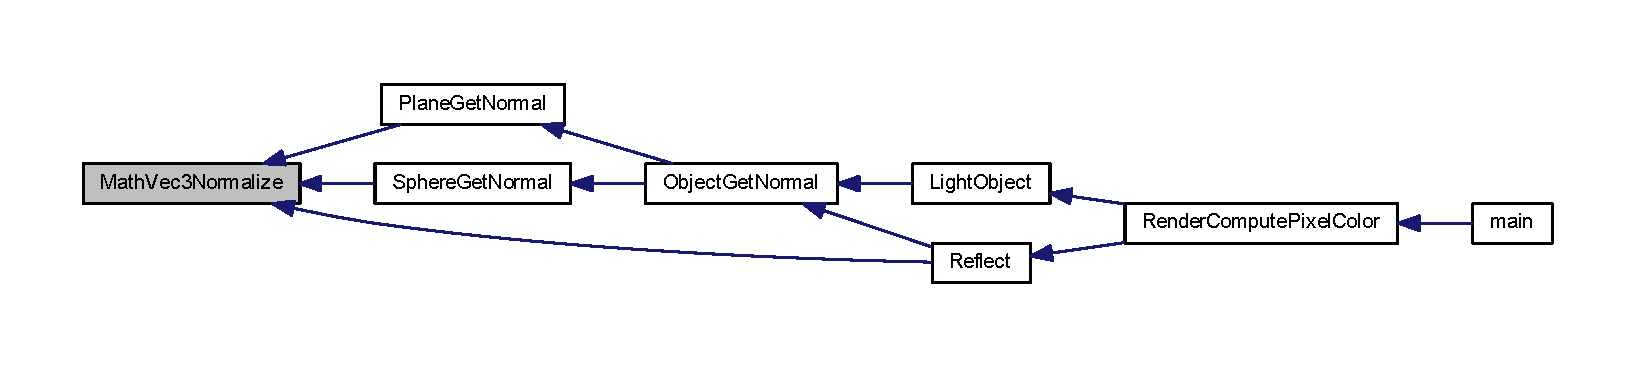
\includegraphics[width=350pt]{raymath_8h_a075c2db2a273d9e2ab085f4cba6fbf9f_icgraph}
\end{center}
\end{figure}


\index{raymath.\+h@{raymath.\+h}!Math\+Vec3\+Scale@{Math\+Vec3\+Scale}}
\index{Math\+Vec3\+Scale@{Math\+Vec3\+Scale}!raymath.\+h@{raymath.\+h}}
\subsubsection[{\texorpdfstring{Math\+Vec3\+Scale(vec3\+\_\+t a, number c)}{MathVec3Scale(vec3_t a, number c)}}]{\setlength{\rightskip}{0pt plus 5cm}{\bf vec3\+\_\+t} Math\+Vec3\+Scale (
\begin{DoxyParamCaption}
\item[{{\bf vec3\+\_\+t}}]{a, }
\item[{{\bf number}}]{c}
\end{DoxyParamCaption}
)}\hypertarget{raymath_8h_a414c0be0d1f209943c3ecbbae79002d2}{}\label{raymath_8h_a414c0be0d1f209943c3ecbbae79002d2}


Scale a 3D vector (multiply by a scalar) 


\begin{DoxyParams}{Parameters}
{\em a} & 3D vector \\
\hline
{\em c} & scalar \\
\hline
\end{DoxyParams}
\begin{DoxyReturn}{Returns}
resulting 3D vector (a x c) 
\end{DoxyReturn}


Definition at line 39 of file raymath.\+c.



Here is the call graph for this function\+:\nopagebreak
\begin{figure}[H]
\begin{center}
\leavevmode
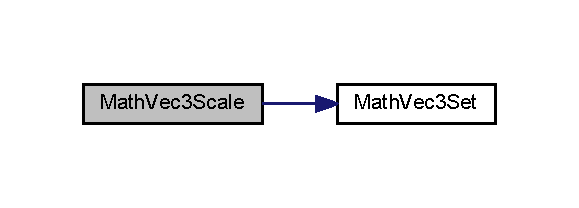
\includegraphics[width=278pt]{raymath_8h_a414c0be0d1f209943c3ecbbae79002d2_cgraph}
\end{center}
\end{figure}




Here is the caller graph for this function\+:\nopagebreak
\begin{figure}[H]
\begin{center}
\leavevmode
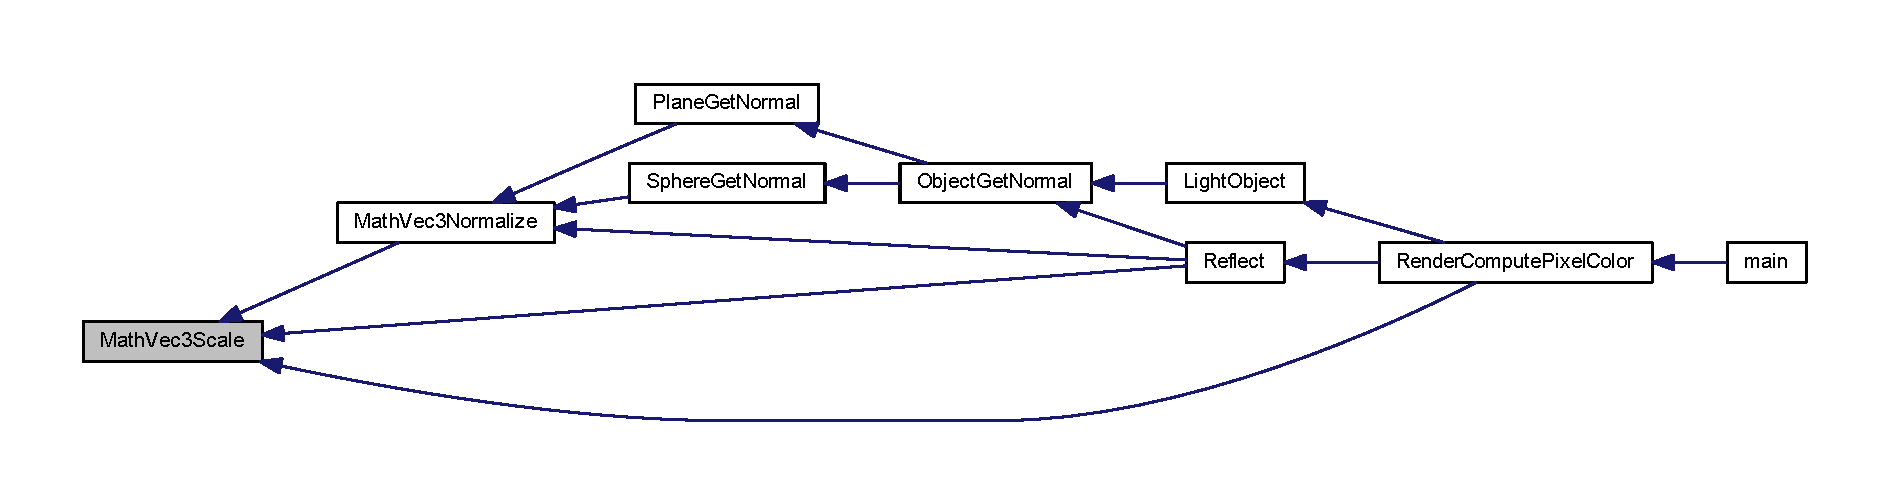
\includegraphics[width=350pt]{raymath_8h_a414c0be0d1f209943c3ecbbae79002d2_icgraph}
\end{center}
\end{figure}


\index{raymath.\+h@{raymath.\+h}!Math\+Vec3\+Set@{Math\+Vec3\+Set}}
\index{Math\+Vec3\+Set@{Math\+Vec3\+Set}!raymath.\+h@{raymath.\+h}}
\subsubsection[{\texorpdfstring{Math\+Vec3\+Set(number x, number y, number z)}{MathVec3Set(number x, number y, number z)}}]{\setlength{\rightskip}{0pt plus 5cm}{\bf vec3\+\_\+t} Math\+Vec3\+Set (
\begin{DoxyParamCaption}
\item[{{\bf number}}]{x, }
\item[{{\bf number}}]{y, }
\item[{{\bf number}}]{z}
\end{DoxyParamCaption}
)}\hypertarget{raymath_8h_a0c3b96d5e78c8899245e367835c0e1b4}{}\label{raymath_8h_a0c3b96d5e78c8899245e367835c0e1b4}


Set a 3D vector. 


\begin{DoxyParams}{Parameters}
{\em x} & x component \\
\hline
{\em y} & y component \\
\hline
{\em z} & z component \\
\hline
\end{DoxyParams}
\begin{DoxyReturn}{Returns}
3D vector 
\end{DoxyReturn}


Definition at line 21 of file raymath.\+c.



Here is the caller graph for this function\+:\nopagebreak
\begin{figure}[H]
\begin{center}
\leavevmode
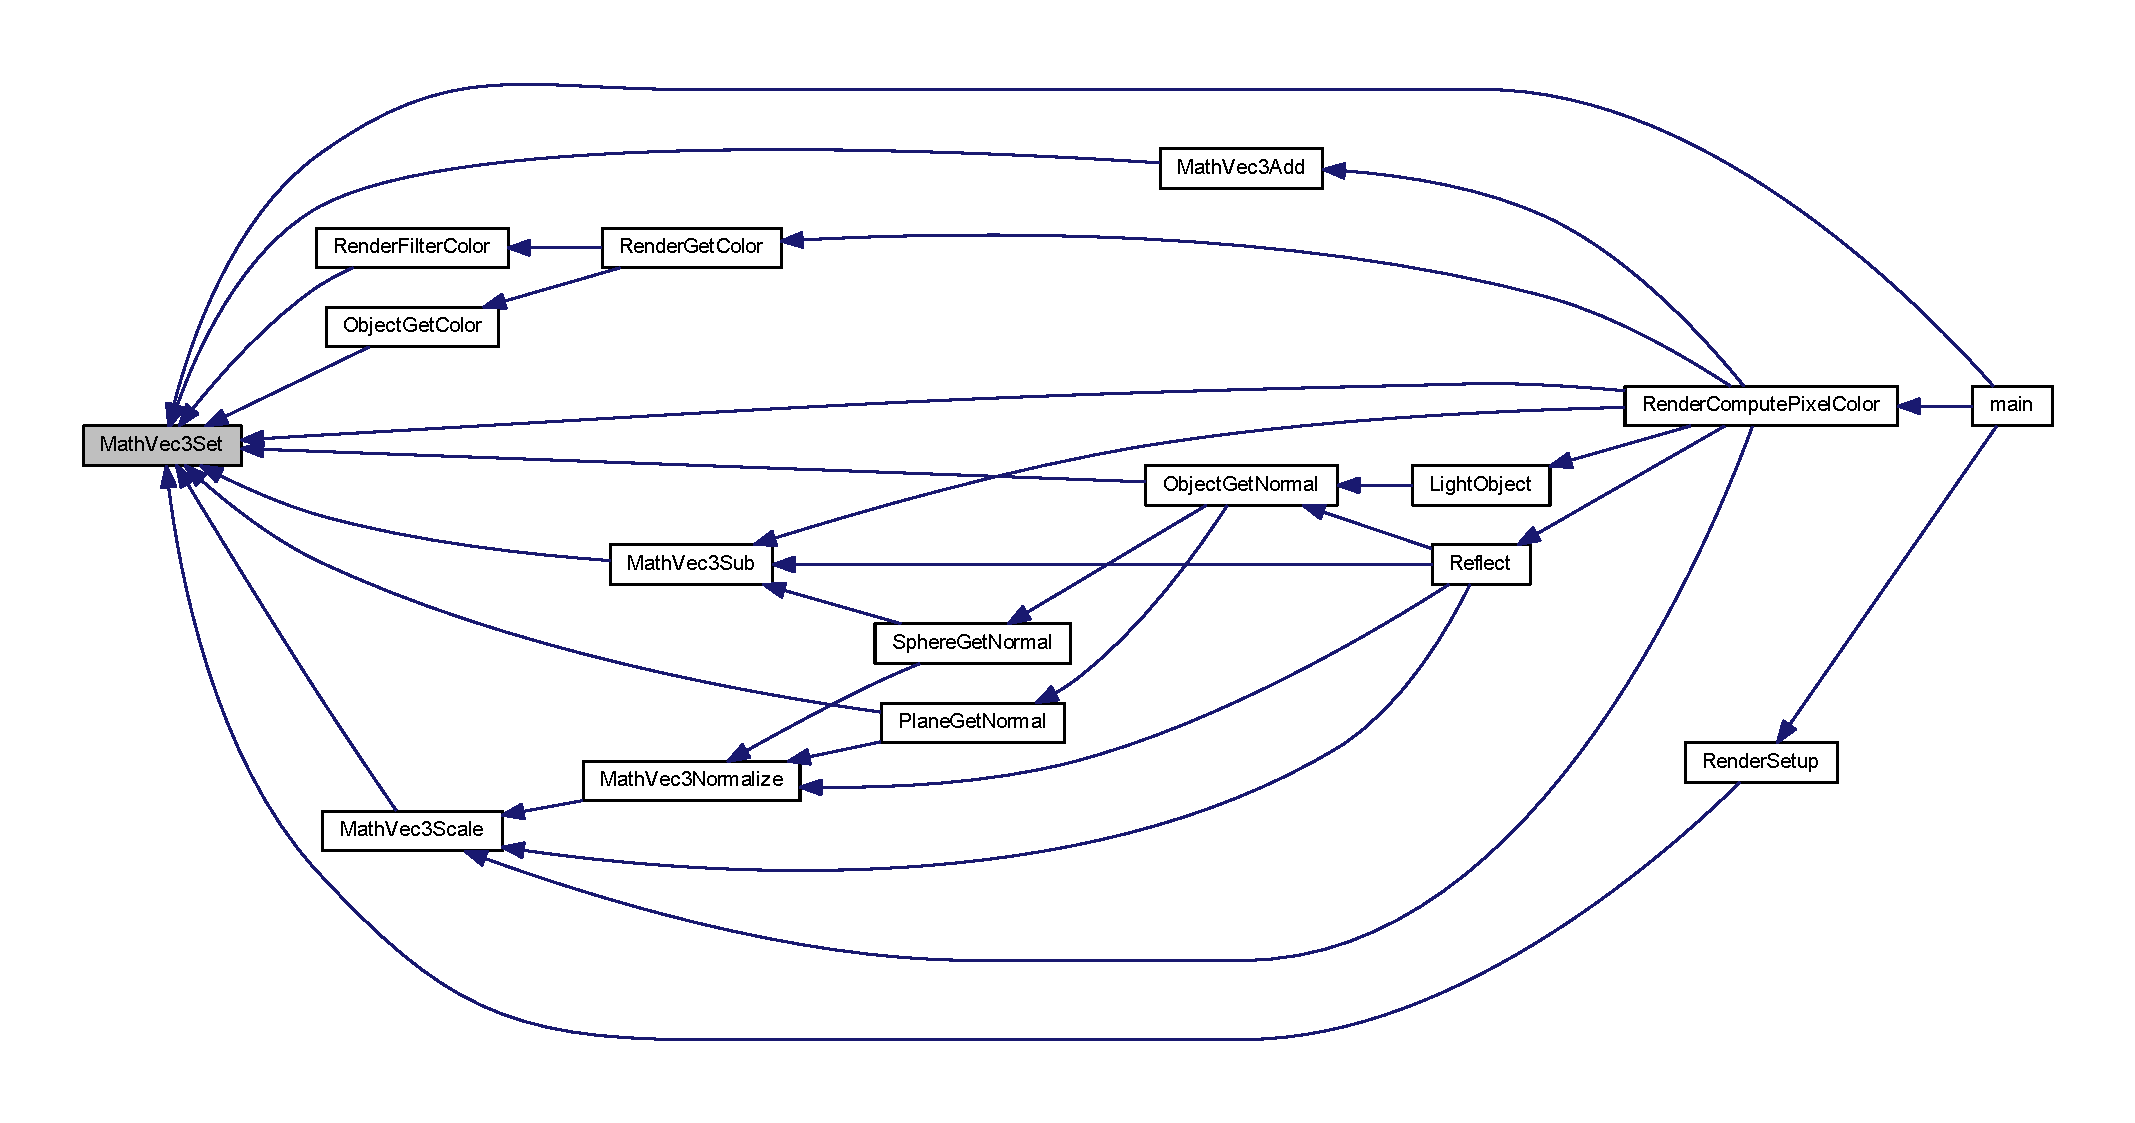
\includegraphics[width=350pt]{raymath_8h_a0c3b96d5e78c8899245e367835c0e1b4_icgraph}
\end{center}
\end{figure}


\index{raymath.\+h@{raymath.\+h}!Math\+Vec3\+Sub@{Math\+Vec3\+Sub}}
\index{Math\+Vec3\+Sub@{Math\+Vec3\+Sub}!raymath.\+h@{raymath.\+h}}
\subsubsection[{\texorpdfstring{Math\+Vec3\+Sub(vec3\+\_\+t a, vec3\+\_\+t b)}{MathVec3Sub(vec3_t a, vec3_t b)}}]{\setlength{\rightskip}{0pt plus 5cm}{\bf vec3\+\_\+t} Math\+Vec3\+Sub (
\begin{DoxyParamCaption}
\item[{{\bf vec3\+\_\+t}}]{a, }
\item[{{\bf vec3\+\_\+t}}]{b}
\end{DoxyParamCaption}
)}\hypertarget{raymath_8h_afc53ea0adde49d6b23d3d20f7242ce3b}{}\label{raymath_8h_afc53ea0adde49d6b23d3d20f7242ce3b}


Subtract two 3D vectors. 


\begin{DoxyParams}{Parameters}
{\em a} & 3D vector \\
\hline
{\em b} & 3D vector \\
\hline
\end{DoxyParams}
\begin{DoxyReturn}{Returns}
resulting 3D vector (a -\/ b) 
\end{DoxyReturn}


Definition at line 34 of file raymath.\+c.



Here is the call graph for this function\+:\nopagebreak
\begin{figure}[H]
\begin{center}
\leavevmode
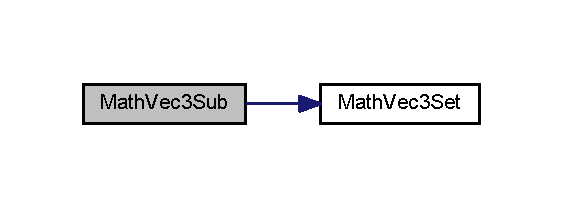
\includegraphics[width=270pt]{raymath_8h_afc53ea0adde49d6b23d3d20f7242ce3b_cgraph}
\end{center}
\end{figure}




Here is the caller graph for this function\+:\nopagebreak
\begin{figure}[H]
\begin{center}
\leavevmode
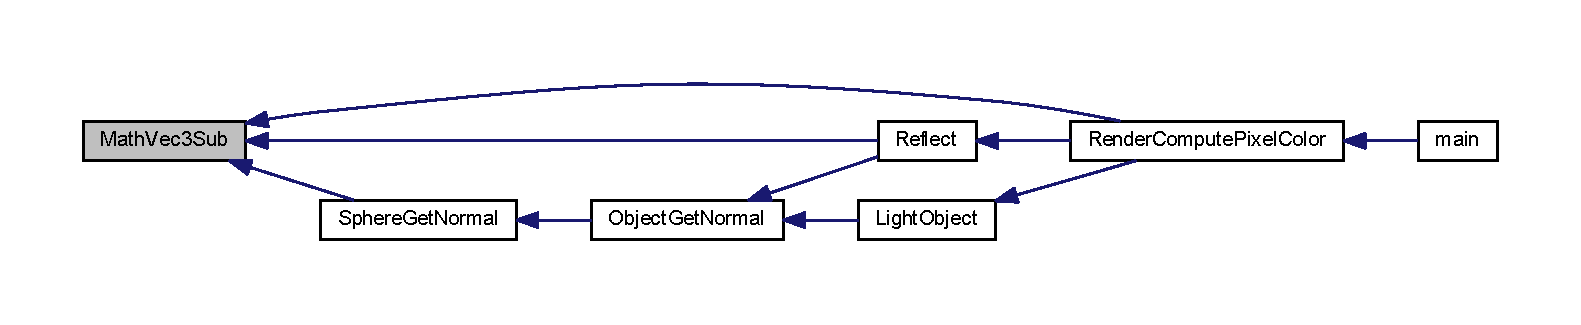
\includegraphics[width=350pt]{raymath_8h_afc53ea0adde49d6b23d3d20f7242ce3b_icgraph}
\end{center}
\end{figure}



\hypertarget{raymathfix_8h}{}\section{Includes/raymathfix.h File Reference}
\label{raymathfix_8h}\index{Includes/raymathfix.\+h@{Includes/raymathfix.\+h}}


Raytracer fix math.  


{\ttfamily \#include $<$stdio.\+h$>$}\\*
{\ttfamily \#include $<$stdbool.\+h$>$}\\*
{\ttfamily \#include $<$stdlib.\+h$>$}\\*
{\ttfamily \#include $<$math.\+h$>$}\\*
{\ttfamily \#include \char`\"{}raymath.\+h\char`\"{}}\\*
Include dependency graph for raymathfix.\+h\+:\nopagebreak
\begin{figure}[H]
\begin{center}
\leavevmode
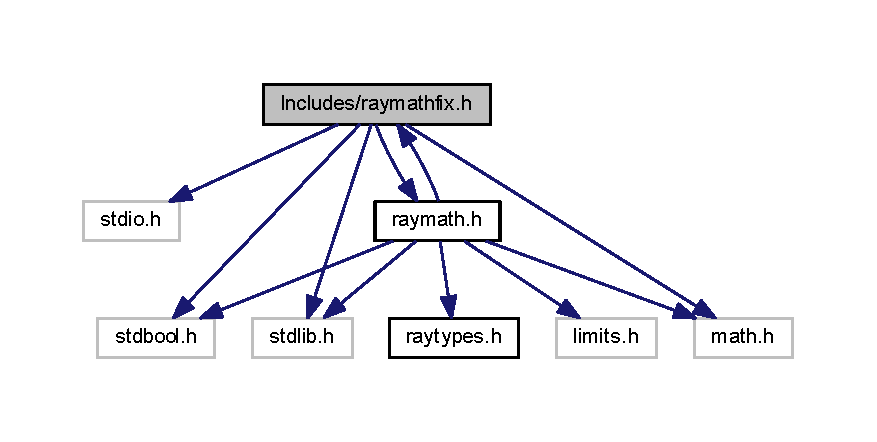
\includegraphics[width=350pt]{raymathfix_8h__incl}
\end{center}
\end{figure}
This graph shows which files directly or indirectly include this file\+:
\nopagebreak
\begin{figure}[H]
\begin{center}
\leavevmode
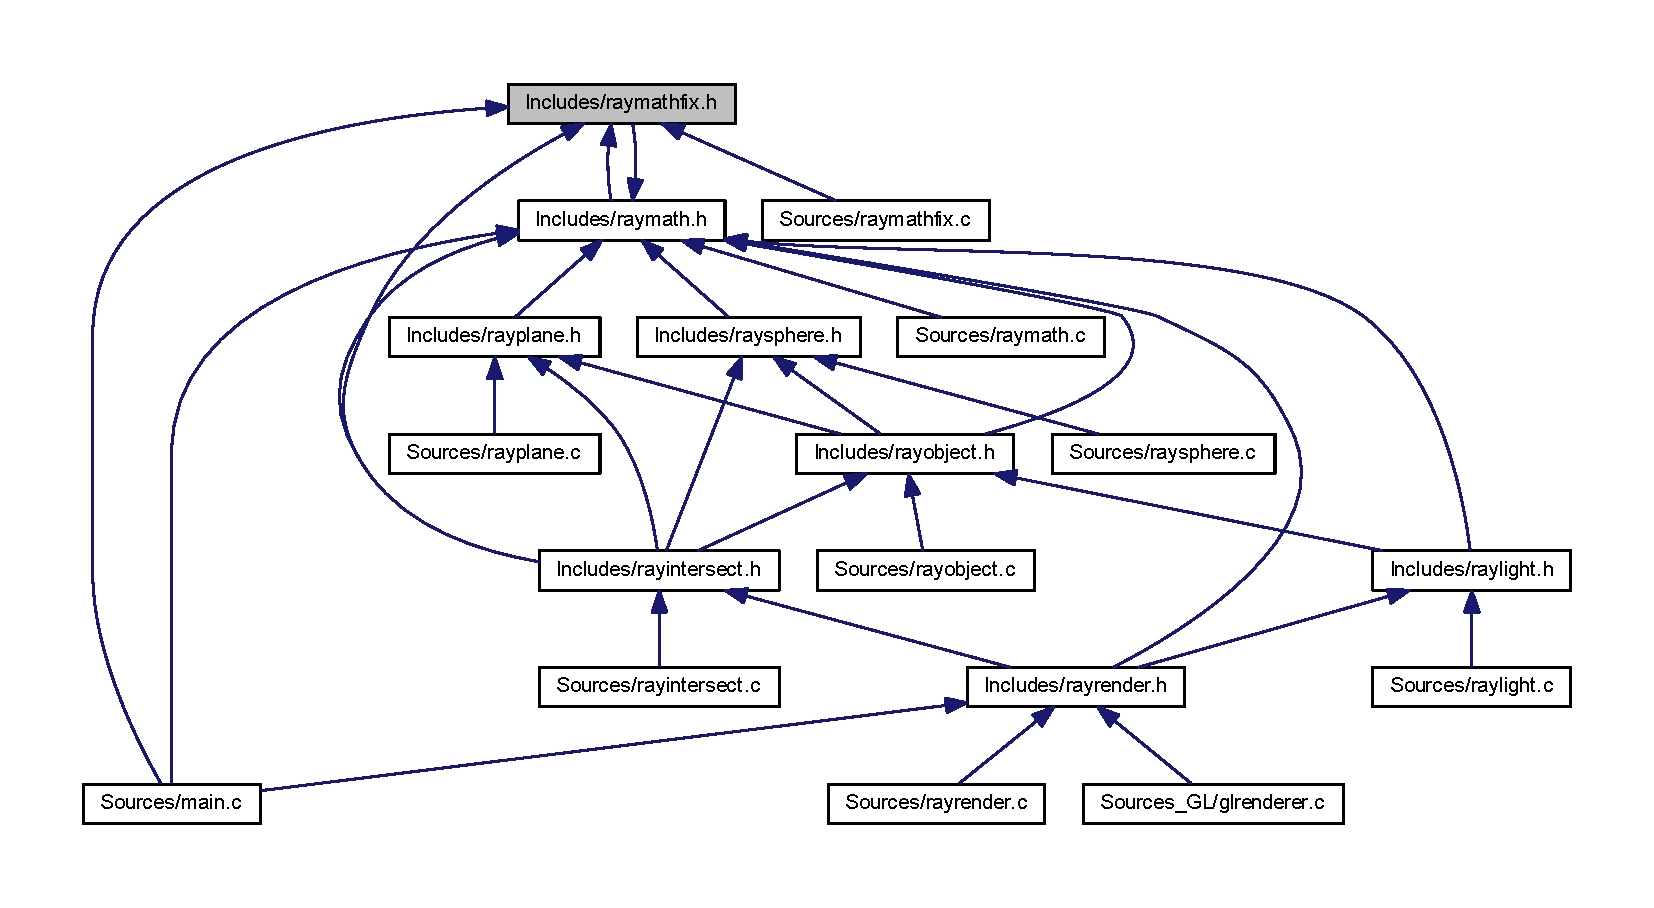
\includegraphics[width=350pt]{raymathfix_8h__dep__incl}
\end{center}
\end{figure}
\subsection*{Macros}
\begin{DoxyCompactItemize}
\item 
\#define \hyperlink{raymathfix_8h_a8edc3240c157eecf1131299de27dea7a}{F\+I\+X\+\_\+\+S\+H\+I\+FT}~12
\begin{DoxyCompactList}\small\item\em Fixed point number of fractional bits. \end{DoxyCompactList}\item 
\#define \hyperlink{raymathfix_8h_a2074879063dde33e28fb3ccffdd5e6e4}{F\+I\+X\+\_\+\+S\+C\+A\+LE}~( 1 $<$$<$ \hyperlink{raymathfix_8h_a8edc3240c157eecf1131299de27dea7a}{F\+I\+X\+\_\+\+S\+H\+I\+FT} )
\item 
\#define \hyperlink{raymathfix_8h_a88d27014adc2dc791584fcb71ff34641}{F\+I\+X\+\_\+\+M\+A\+SK}~( \hyperlink{raymathfix_8h_a2074879063dde33e28fb3ccffdd5e6e4}{F\+I\+X\+\_\+\+S\+C\+A\+LE} -\/ 1 )
\item 
\#define \hyperlink{raymathfix_8h_adc9777294ed3349f0ac3b77b58cf24e2}{F\+I\+X\+\_\+\+S\+C\+A\+L\+EF}~( (float)\hyperlink{raymathfix_8h_a2074879063dde33e28fb3ccffdd5e6e4}{F\+I\+X\+\_\+\+S\+C\+A\+LE} )
\item 
\#define \hyperlink{raymathfix_8h_afb3623ba637d3ac3a3cf737146aace15}{F\+I\+X\+\_\+\+S\+C\+A\+L\+E\+F\+\_\+\+I\+NV}~( 1.\+0f / F\+I\+X\+\_\+\+S\+C\+A\+L\+E\+F	)
\item 
\#define \hyperlink{raymathfix_8h_a4ceea0e31ae25efeaa7a4c76d85ed950}{F\+I\+X\+\_\+\+O\+NE}~\hyperlink{raymathfix_8h_a2074879063dde33e28fb3ccffdd5e6e4}{F\+I\+X\+\_\+\+S\+C\+A\+LE}
\item 
\#define \hyperlink{raymathfix_8h_ab5cadba2a8639b9ef54ab46b3155799c}{Math\+Float2\+Fix}(f)~(\hyperlink{raymath_8h_aa97c1f529dc5a11a78758184c84a39c9}{number})( f $\ast$ \hyperlink{raymathfix_8h_adc9777294ed3349f0ac3b77b58cf24e2}{F\+I\+X\+\_\+\+S\+C\+A\+L\+EF} )
\begin{DoxyCompactList}\small\item\em Convert a floating point number to a fixed point number. \end{DoxyCompactList}\item 
\#define \hyperlink{raymathfix_8h_a662a769f40ac43a3d5e1afeda0f0e9c9}{Math\+Fix\+Add}(fa,  fb)~(\hyperlink{raymath_8h_aa97c1f529dc5a11a78758184c84a39c9}{number})( fa + fb )
\begin{DoxyCompactList}\small\item\em Add two fixed point number. \end{DoxyCompactList}\item 
\#define \hyperlink{raymathfix_8h_a9efdd30e8c235b4e7d710adfa2b933dc}{Math\+Fix\+Sub}(fa,  fb)~(\hyperlink{raymath_8h_aa97c1f529dc5a11a78758184c84a39c9}{number})( fa -\/ fb )
\begin{DoxyCompactList}\small\item\em Subtract two fixed point number. \end{DoxyCompactList}\item 
\#define \hyperlink{raymathfix_8h_a8d93126fdac6ca6825b80576bed9a7c5}{Math\+Fix\+Mul}(fa,  fb)~(\hyperlink{raymath_8h_aa97c1f529dc5a11a78758184c84a39c9}{number})( ( fa $\ast$ fb ) $>$$>$ \hyperlink{raymathfix_8h_a8edc3240c157eecf1131299de27dea7a}{F\+I\+X\+\_\+\+S\+H\+I\+FT} )
\begin{DoxyCompactList}\small\item\em Multiply two fixed point number. \end{DoxyCompactList}\item 
\#define \hyperlink{raymathfix_8h_a00f0fef6f042f8aea5ce731a68a3316a}{Math\+Fix\+Div}(fa,  fb)~( ( (\hyperlink{raymath_8h_aa97c1f529dc5a11a78758184c84a39c9}{number})fa ) $<$$<$ \hyperlink{raymathfix_8h_a8edc3240c157eecf1131299de27dea7a}{F\+I\+X\+\_\+\+S\+H\+I\+FT} ) / ( ( fb == 0 ) ? 1 \+: fb )
\begin{DoxyCompactList}\small\item\em Divide two fixed point number. \end{DoxyCompactList}\item 
\#define \hyperlink{raymathfix_8h_afebd8dc45d13413b695ac0bef6593629}{Math\+Int2\+Fix}(d)~(\hyperlink{raytypes_8h_abab37cf41841dab8dc81b8da87acd6c5}{fixed})( d $<$$<$ \hyperlink{raymathfix_8h_a8edc3240c157eecf1131299de27dea7a}{F\+I\+X\+\_\+\+S\+H\+I\+FT} )
\begin{DoxyCompactList}\small\item\em Convert a integer to a fixed point number. \end{DoxyCompactList}\item 
\#define \hyperlink{raymathfix_8h_a942ebb7dde9c1d71c1e80fcb236dbc5b}{Math\+Fix2\+Uint}(fix)~(\hyperlink{raytypes_8h_a0c0a490ab7fa397be6c764a935cc5ea4}{u32\+\_\+t})( fix $>$$>$ \hyperlink{raymathfix_8h_a8edc3240c157eecf1131299de27dea7a}{F\+I\+X\+\_\+\+S\+H\+I\+FT} )
\begin{DoxyCompactList}\small\item\em Convert a fixed point number to an unsigned integer. \end{DoxyCompactList}\item 
\#define \hyperlink{raymathfix_8h_a9726ebedebc4c86b01ec631d1c241bfc}{Math\+Fix2\+U\+Frac}(fix)~(\hyperlink{raytypes_8h_a0c0a490ab7fa397be6c764a935cc5ea4}{u32\+\_\+t})( fix \& \hyperlink{raymathfix_8h_a88d27014adc2dc791584fcb71ff34641}{F\+I\+X\+\_\+\+M\+A\+SK} )
\begin{DoxyCompactList}\small\item\em Convert a fixed point fractional part to an unsigned integer. \end{DoxyCompactList}\item 
\#define \hyperlink{raymathfix_8h_a0e590211d6e7798c4db9f0551f432898}{Math\+Fix2\+Int}(fix)~(int)( fix / \hyperlink{raymathfix_8h_a2074879063dde33e28fb3ccffdd5e6e4}{F\+I\+X\+\_\+\+S\+C\+A\+LE} )
\begin{DoxyCompactList}\small\item\em Convert a fixed point number part to a signed integer. \end{DoxyCompactList}\item 
\#define \hyperlink{raymathfix_8h_a328874c73d54ce44afc7c60a7054941c}{Math\+Fix2\+Float}(fix)~(float)( fix / \hyperlink{raymathfix_8h_adc9777294ed3349f0ac3b77b58cf24e2}{F\+I\+X\+\_\+\+S\+C\+A\+L\+EF} )
\begin{DoxyCompactList}\small\item\em Convert a fixed point number to a floating point number. \end{DoxyCompactList}\end{DoxyCompactItemize}


\subsection{Detailed Description}
Raytracer fix math. 

\begin{DoxyAuthor}{Author}
J. Crenne \& C. Leroux 
\end{DoxyAuthor}
\begin{DoxyVersion}{Version}
1.\+0 
\end{DoxyVersion}
\begin{DoxyDate}{Date}
February 2016 
\end{DoxyDate}


\subsection{Macro Definition Documentation}
\index{raymathfix.\+h@{raymathfix.\+h}!F\+I\+X\+\_\+\+M\+A\+SK@{F\+I\+X\+\_\+\+M\+A\+SK}}
\index{F\+I\+X\+\_\+\+M\+A\+SK@{F\+I\+X\+\_\+\+M\+A\+SK}!raymathfix.\+h@{raymathfix.\+h}}
\subsubsection[{\texorpdfstring{F\+I\+X\+\_\+\+M\+A\+SK}{FIX_MASK}}]{\setlength{\rightskip}{0pt plus 5cm}\#define F\+I\+X\+\_\+\+M\+A\+SK~( {\bf F\+I\+X\+\_\+\+S\+C\+A\+LE} -\/ 1 )}\hypertarget{raymathfix_8h_a88d27014adc2dc791584fcb71ff34641}{}\label{raymathfix_8h_a88d27014adc2dc791584fcb71ff34641}


Definition at line 26 of file raymathfix.\+h.

\index{raymathfix.\+h@{raymathfix.\+h}!F\+I\+X\+\_\+\+O\+NE@{F\+I\+X\+\_\+\+O\+NE}}
\index{F\+I\+X\+\_\+\+O\+NE@{F\+I\+X\+\_\+\+O\+NE}!raymathfix.\+h@{raymathfix.\+h}}
\subsubsection[{\texorpdfstring{F\+I\+X\+\_\+\+O\+NE}{FIX_ONE}}]{\setlength{\rightskip}{0pt plus 5cm}\#define F\+I\+X\+\_\+\+O\+NE~{\bf F\+I\+X\+\_\+\+S\+C\+A\+LE}}\hypertarget{raymathfix_8h_a4ceea0e31ae25efeaa7a4c76d85ed950}{}\label{raymathfix_8h_a4ceea0e31ae25efeaa7a4c76d85ed950}


Definition at line 29 of file raymathfix.\+h.

\index{raymathfix.\+h@{raymathfix.\+h}!F\+I\+X\+\_\+\+S\+C\+A\+LE@{F\+I\+X\+\_\+\+S\+C\+A\+LE}}
\index{F\+I\+X\+\_\+\+S\+C\+A\+LE@{F\+I\+X\+\_\+\+S\+C\+A\+LE}!raymathfix.\+h@{raymathfix.\+h}}
\subsubsection[{\texorpdfstring{F\+I\+X\+\_\+\+S\+C\+A\+LE}{FIX_SCALE}}]{\setlength{\rightskip}{0pt plus 5cm}\#define F\+I\+X\+\_\+\+S\+C\+A\+LE~( 1 $<$$<$ {\bf F\+I\+X\+\_\+\+S\+H\+I\+FT} )}\hypertarget{raymathfix_8h_a2074879063dde33e28fb3ccffdd5e6e4}{}\label{raymathfix_8h_a2074879063dde33e28fb3ccffdd5e6e4}


Definition at line 25 of file raymathfix.\+h.

\index{raymathfix.\+h@{raymathfix.\+h}!F\+I\+X\+\_\+\+S\+C\+A\+L\+EF@{F\+I\+X\+\_\+\+S\+C\+A\+L\+EF}}
\index{F\+I\+X\+\_\+\+S\+C\+A\+L\+EF@{F\+I\+X\+\_\+\+S\+C\+A\+L\+EF}!raymathfix.\+h@{raymathfix.\+h}}
\subsubsection[{\texorpdfstring{F\+I\+X\+\_\+\+S\+C\+A\+L\+EF}{FIX_SCALEF}}]{\setlength{\rightskip}{0pt plus 5cm}\#define F\+I\+X\+\_\+\+S\+C\+A\+L\+EF~( (float){\bf F\+I\+X\+\_\+\+S\+C\+A\+LE} )}\hypertarget{raymathfix_8h_adc9777294ed3349f0ac3b77b58cf24e2}{}\label{raymathfix_8h_adc9777294ed3349f0ac3b77b58cf24e2}


Definition at line 27 of file raymathfix.\+h.

\index{raymathfix.\+h@{raymathfix.\+h}!F\+I\+X\+\_\+\+S\+C\+A\+L\+E\+F\+\_\+\+I\+NV@{F\+I\+X\+\_\+\+S\+C\+A\+L\+E\+F\+\_\+\+I\+NV}}
\index{F\+I\+X\+\_\+\+S\+C\+A\+L\+E\+F\+\_\+\+I\+NV@{F\+I\+X\+\_\+\+S\+C\+A\+L\+E\+F\+\_\+\+I\+NV}!raymathfix.\+h@{raymathfix.\+h}}
\subsubsection[{\texorpdfstring{F\+I\+X\+\_\+\+S\+C\+A\+L\+E\+F\+\_\+\+I\+NV}{FIX_SCALEF_INV}}]{\setlength{\rightskip}{0pt plus 5cm}\#define F\+I\+X\+\_\+\+S\+C\+A\+L\+E\+F\+\_\+\+I\+NV~( 1.\+0f / F\+I\+X\+\_\+\+S\+C\+A\+L\+E\+F	)}\hypertarget{raymathfix_8h_afb3623ba637d3ac3a3cf737146aace15}{}\label{raymathfix_8h_afb3623ba637d3ac3a3cf737146aace15}


Definition at line 28 of file raymathfix.\+h.

\index{raymathfix.\+h@{raymathfix.\+h}!F\+I\+X\+\_\+\+S\+H\+I\+FT@{F\+I\+X\+\_\+\+S\+H\+I\+FT}}
\index{F\+I\+X\+\_\+\+S\+H\+I\+FT@{F\+I\+X\+\_\+\+S\+H\+I\+FT}!raymathfix.\+h@{raymathfix.\+h}}
\subsubsection[{\texorpdfstring{F\+I\+X\+\_\+\+S\+H\+I\+FT}{FIX_SHIFT}}]{\setlength{\rightskip}{0pt plus 5cm}\#define F\+I\+X\+\_\+\+S\+H\+I\+FT~12}\hypertarget{raymathfix_8h_a8edc3240c157eecf1131299de27dea7a}{}\label{raymathfix_8h_a8edc3240c157eecf1131299de27dea7a}


Fixed point number of fractional bits. 



Definition at line 23 of file raymathfix.\+h.

\index{raymathfix.\+h@{raymathfix.\+h}!Math\+Fix2\+Float@{Math\+Fix2\+Float}}
\index{Math\+Fix2\+Float@{Math\+Fix2\+Float}!raymathfix.\+h@{raymathfix.\+h}}
\subsubsection[{\texorpdfstring{Math\+Fix2\+Float}{MathFix2Float}}]{\setlength{\rightskip}{0pt plus 5cm}\#define Math\+Fix2\+Float(
\begin{DoxyParamCaption}
\item[{}]{fix}
\end{DoxyParamCaption}
)~(float)( fix / {\bf F\+I\+X\+\_\+\+S\+C\+A\+L\+EF} )}\hypertarget{raymathfix_8h_a328874c73d54ce44afc7c60a7054941c}{}\label{raymathfix_8h_a328874c73d54ce44afc7c60a7054941c}


Convert a fixed point number to a floating point number. 



Definition at line 89 of file raymathfix.\+h.

\index{raymathfix.\+h@{raymathfix.\+h}!Math\+Fix2\+Int@{Math\+Fix2\+Int}}
\index{Math\+Fix2\+Int@{Math\+Fix2\+Int}!raymathfix.\+h@{raymathfix.\+h}}
\subsubsection[{\texorpdfstring{Math\+Fix2\+Int}{MathFix2Int}}]{\setlength{\rightskip}{0pt plus 5cm}\#define Math\+Fix2\+Int(
\begin{DoxyParamCaption}
\item[{}]{fix}
\end{DoxyParamCaption}
)~(int)( fix / {\bf F\+I\+X\+\_\+\+S\+C\+A\+LE} )}\hypertarget{raymathfix_8h_a0e590211d6e7798c4db9f0551f432898}{}\label{raymathfix_8h_a0e590211d6e7798c4db9f0551f432898}


Convert a fixed point number part to a signed integer. 



Definition at line 83 of file raymathfix.\+h.

\index{raymathfix.\+h@{raymathfix.\+h}!Math\+Fix2\+U\+Frac@{Math\+Fix2\+U\+Frac}}
\index{Math\+Fix2\+U\+Frac@{Math\+Fix2\+U\+Frac}!raymathfix.\+h@{raymathfix.\+h}}
\subsubsection[{\texorpdfstring{Math\+Fix2\+U\+Frac}{MathFix2UFrac}}]{\setlength{\rightskip}{0pt plus 5cm}\#define Math\+Fix2\+U\+Frac(
\begin{DoxyParamCaption}
\item[{}]{fix}
\end{DoxyParamCaption}
)~({\bf u32\+\_\+t})( fix \& {\bf F\+I\+X\+\_\+\+M\+A\+SK} )}\hypertarget{raymathfix_8h_a9726ebedebc4c86b01ec631d1c241bfc}{}\label{raymathfix_8h_a9726ebedebc4c86b01ec631d1c241bfc}


Convert a fixed point fractional part to an unsigned integer. 



Definition at line 77 of file raymathfix.\+h.

\index{raymathfix.\+h@{raymathfix.\+h}!Math\+Fix2\+Uint@{Math\+Fix2\+Uint}}
\index{Math\+Fix2\+Uint@{Math\+Fix2\+Uint}!raymathfix.\+h@{raymathfix.\+h}}
\subsubsection[{\texorpdfstring{Math\+Fix2\+Uint}{MathFix2Uint}}]{\setlength{\rightskip}{0pt plus 5cm}\#define Math\+Fix2\+Uint(
\begin{DoxyParamCaption}
\item[{}]{fix}
\end{DoxyParamCaption}
)~({\bf u32\+\_\+t})( fix $>$$>$ {\bf F\+I\+X\+\_\+\+S\+H\+I\+FT} )}\hypertarget{raymathfix_8h_a942ebb7dde9c1d71c1e80fcb236dbc5b}{}\label{raymathfix_8h_a942ebb7dde9c1d71c1e80fcb236dbc5b}


Convert a fixed point number to an unsigned integer. 



Definition at line 71 of file raymathfix.\+h.

\index{raymathfix.\+h@{raymathfix.\+h}!Math\+Fix\+Add@{Math\+Fix\+Add}}
\index{Math\+Fix\+Add@{Math\+Fix\+Add}!raymathfix.\+h@{raymathfix.\+h}}
\subsubsection[{\texorpdfstring{Math\+Fix\+Add}{MathFixAdd}}]{\setlength{\rightskip}{0pt plus 5cm}\#define Math\+Fix\+Add(
\begin{DoxyParamCaption}
\item[{}]{fa, }
\item[{}]{fb}
\end{DoxyParamCaption}
)~({\bf number})( fa + fb )}\hypertarget{raymathfix_8h_a662a769f40ac43a3d5e1afeda0f0e9c9}{}\label{raymathfix_8h_a662a769f40ac43a3d5e1afeda0f0e9c9}


Add two fixed point number. 



Definition at line 41 of file raymathfix.\+h.

\index{raymathfix.\+h@{raymathfix.\+h}!Math\+Fix\+Div@{Math\+Fix\+Div}}
\index{Math\+Fix\+Div@{Math\+Fix\+Div}!raymathfix.\+h@{raymathfix.\+h}}
\subsubsection[{\texorpdfstring{Math\+Fix\+Div}{MathFixDiv}}]{\setlength{\rightskip}{0pt plus 5cm}\#define Math\+Fix\+Div(
\begin{DoxyParamCaption}
\item[{}]{fa, }
\item[{}]{fb}
\end{DoxyParamCaption}
)~( ( ({\bf number})fa ) $<$$<$ {\bf F\+I\+X\+\_\+\+S\+H\+I\+FT} ) / ( ( fb == 0 ) ? 1 \+: fb )}\hypertarget{raymathfix_8h_a00f0fef6f042f8aea5ce731a68a3316a}{}\label{raymathfix_8h_a00f0fef6f042f8aea5ce731a68a3316a}


Divide two fixed point number. 



Definition at line 59 of file raymathfix.\+h.

\index{raymathfix.\+h@{raymathfix.\+h}!Math\+Fix\+Mul@{Math\+Fix\+Mul}}
\index{Math\+Fix\+Mul@{Math\+Fix\+Mul}!raymathfix.\+h@{raymathfix.\+h}}
\subsubsection[{\texorpdfstring{Math\+Fix\+Mul}{MathFixMul}}]{\setlength{\rightskip}{0pt plus 5cm}\#define Math\+Fix\+Mul(
\begin{DoxyParamCaption}
\item[{}]{fa, }
\item[{}]{fb}
\end{DoxyParamCaption}
)~({\bf number})( ( fa $\ast$ fb ) $>$$>$ {\bf F\+I\+X\+\_\+\+S\+H\+I\+FT} )}\hypertarget{raymathfix_8h_a8d93126fdac6ca6825b80576bed9a7c5}{}\label{raymathfix_8h_a8d93126fdac6ca6825b80576bed9a7c5}


Multiply two fixed point number. 



Definition at line 53 of file raymathfix.\+h.

\index{raymathfix.\+h@{raymathfix.\+h}!Math\+Fix\+Sub@{Math\+Fix\+Sub}}
\index{Math\+Fix\+Sub@{Math\+Fix\+Sub}!raymathfix.\+h@{raymathfix.\+h}}
\subsubsection[{\texorpdfstring{Math\+Fix\+Sub}{MathFixSub}}]{\setlength{\rightskip}{0pt plus 5cm}\#define Math\+Fix\+Sub(
\begin{DoxyParamCaption}
\item[{}]{fa, }
\item[{}]{fb}
\end{DoxyParamCaption}
)~({\bf number})( fa -\/ fb )}\hypertarget{raymathfix_8h_a9efdd30e8c235b4e7d710adfa2b933dc}{}\label{raymathfix_8h_a9efdd30e8c235b4e7d710adfa2b933dc}


Subtract two fixed point number. 



Definition at line 47 of file raymathfix.\+h.

\index{raymathfix.\+h@{raymathfix.\+h}!Math\+Float2\+Fix@{Math\+Float2\+Fix}}
\index{Math\+Float2\+Fix@{Math\+Float2\+Fix}!raymathfix.\+h@{raymathfix.\+h}}
\subsubsection[{\texorpdfstring{Math\+Float2\+Fix}{MathFloat2Fix}}]{\setlength{\rightskip}{0pt plus 5cm}\#define Math\+Float2\+Fix(
\begin{DoxyParamCaption}
\item[{}]{f}
\end{DoxyParamCaption}
)~({\bf number})( f $\ast$ {\bf F\+I\+X\+\_\+\+S\+C\+A\+L\+EF} )}\hypertarget{raymathfix_8h_ab5cadba2a8639b9ef54ab46b3155799c}{}\label{raymathfix_8h_ab5cadba2a8639b9ef54ab46b3155799c}


Convert a floating point number to a fixed point number. 



Definition at line 35 of file raymathfix.\+h.

\index{raymathfix.\+h@{raymathfix.\+h}!Math\+Int2\+Fix@{Math\+Int2\+Fix}}
\index{Math\+Int2\+Fix@{Math\+Int2\+Fix}!raymathfix.\+h@{raymathfix.\+h}}
\subsubsection[{\texorpdfstring{Math\+Int2\+Fix}{MathInt2Fix}}]{\setlength{\rightskip}{0pt plus 5cm}\#define Math\+Int2\+Fix(
\begin{DoxyParamCaption}
\item[{}]{d}
\end{DoxyParamCaption}
)~({\bf fixed})( d $<$$<$ {\bf F\+I\+X\+\_\+\+S\+H\+I\+FT} )}\hypertarget{raymathfix_8h_afebd8dc45d13413b695ac0bef6593629}{}\label{raymathfix_8h_afebd8dc45d13413b695ac0bef6593629}


Convert a integer to a fixed point number. 



Definition at line 65 of file raymathfix.\+h.


\hypertarget{rayobject_8h}{}\section{Includes/rayobject.h File Reference}
\label{rayobject_8h}\index{Includes/rayobject.\+h@{Includes/rayobject.\+h}}


Raytracer objects.  


{\ttfamily \#include \char`\"{}raymath.\+h\char`\"{}}\\*
{\ttfamily \#include \char`\"{}rayplane.\+h\char`\"{}}\\*
{\ttfamily \#include \char`\"{}raysphere.\+h\char`\"{}}\\*
Include dependency graph for rayobject.\+h\+:\nopagebreak
\begin{figure}[H]
\begin{center}
\leavevmode
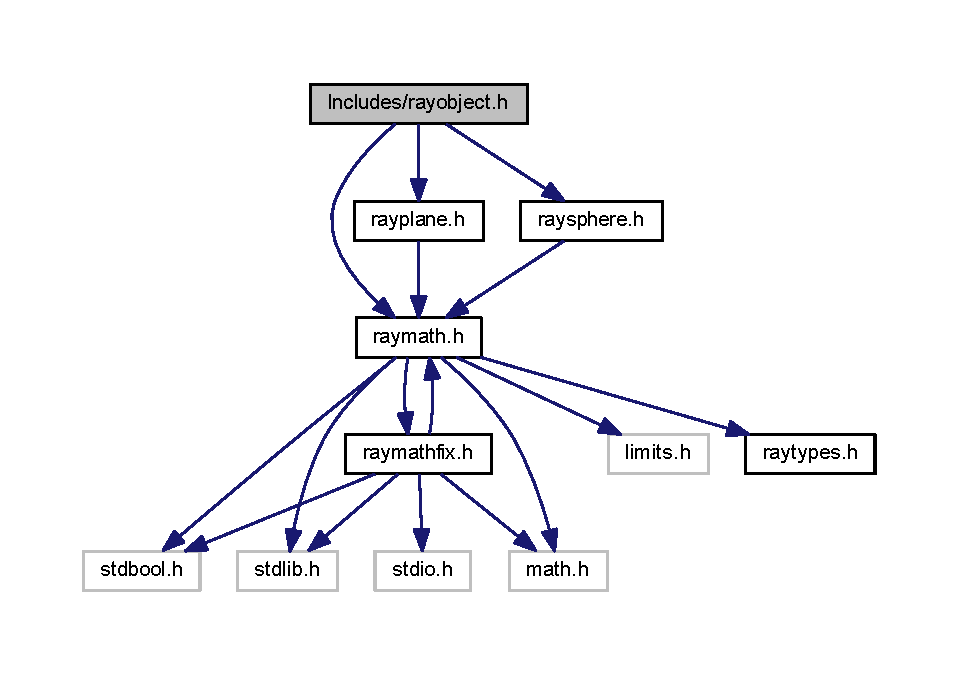
\includegraphics[width=350pt]{rayobject_8h__incl}
\end{center}
\end{figure}
This graph shows which files directly or indirectly include this file\+:
\nopagebreak
\begin{figure}[H]
\begin{center}
\leavevmode
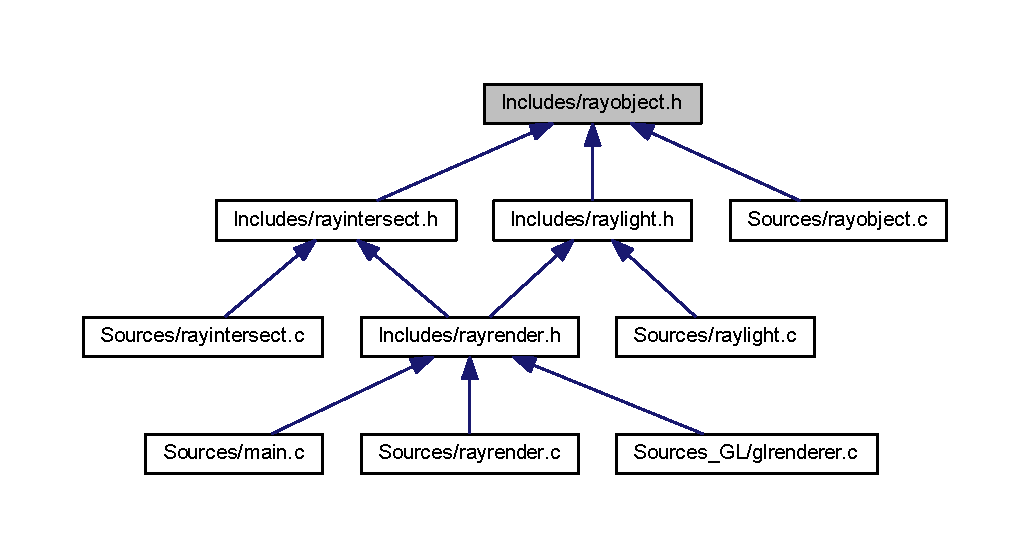
\includegraphics[width=350pt]{rayobject_8h__dep__incl}
\end{center}
\end{figure}
\subsection*{Macros}
\begin{DoxyCompactItemize}
\item 
\#define \hyperlink{rayobject_8h_a95e01e2e5d8068e7de7ea36810be6b5a}{O\+B\+J\+E\+C\+T\+\_\+\+N\+U\+M\+\_\+\+T\+Y\+P\+ES}~2
\begin{DoxyCompactList}\small\item\em Number of object types. \end{DoxyCompactList}\item 
\#define \hyperlink{rayobject_8h_ac35bf2f01a5fa133e9e223ef53f73d4f}{O\+B\+J\+E\+C\+T\+\_\+\+T\+Y\+P\+E\+\_\+\+S\+P\+H\+E\+RE}~0
\begin{DoxyCompactList}\small\item\em Sphere object type constant. \end{DoxyCompactList}\item 
\#define \hyperlink{rayobject_8h_a10e0168abc763a3d84ed11d5a8cee08f}{O\+B\+J\+E\+C\+T\+\_\+\+T\+Y\+P\+E\+\_\+\+P\+L\+A\+NE}~1
\end{DoxyCompactItemize}
\subsection*{Functions}
\begin{DoxyCompactItemize}
\item 
\hyperlink{raytypes_8h_a0c0a490ab7fa397be6c764a935cc5ea4}{u32\+\_\+t} \hyperlink{rayobject_8h_a07163c81c5ae4159950c28fcaa835fc2}{Object\+Get\+Number\+By\+Type} (int type)
\begin{DoxyCompactList}\small\item\em Get the number of objects given a type. \end{DoxyCompactList}\item 
\hyperlink{raymath_8h_afb3684d7701a8417d1a52fd94c84457c}{vec3\+\_\+t} \hyperlink{rayobject_8h_ad5b91bc5eba77d5f29d82147b63bd30f}{Object\+Get\+Normal} (int type, int idx, \hyperlink{raymath_8h_afb3684d7701a8417d1a52fd94c84457c}{vec3\+\_\+t} p, \hyperlink{raymath_8h_afb3684d7701a8417d1a52fd94c84457c}{vec3\+\_\+t} inside)
\begin{DoxyCompactList}\small\item\em Get an object normal. \end{DoxyCompactList}\item 
\hyperlink{raymath_8h_afb3684d7701a8417d1a52fd94c84457c}{vec3\+\_\+t} \hyperlink{rayobject_8h_a85b5e2864495dc8d6fb2089fd6ec183e}{Object\+Get\+Color} (int type, int idx)
\begin{DoxyCompactList}\small\item\em Get an object color. \end{DoxyCompactList}\end{DoxyCompactItemize}


\subsection{Detailed Description}
Raytracer objects. 

\begin{DoxyAuthor}{Author}
J. Crenne \& C. Leroux 
\end{DoxyAuthor}
\begin{DoxyVersion}{Version}
1.\+0 
\end{DoxyVersion}
\begin{DoxyDate}{Date}
February 2016 
\end{DoxyDate}


\subsection{Macro Definition Documentation}
\index{rayobject.\+h@{rayobject.\+h}!O\+B\+J\+E\+C\+T\+\_\+\+N\+U\+M\+\_\+\+T\+Y\+P\+ES@{O\+B\+J\+E\+C\+T\+\_\+\+N\+U\+M\+\_\+\+T\+Y\+P\+ES}}
\index{O\+B\+J\+E\+C\+T\+\_\+\+N\+U\+M\+\_\+\+T\+Y\+P\+ES@{O\+B\+J\+E\+C\+T\+\_\+\+N\+U\+M\+\_\+\+T\+Y\+P\+ES}!rayobject.\+h@{rayobject.\+h}}
\subsubsection[{\texorpdfstring{O\+B\+J\+E\+C\+T\+\_\+\+N\+U\+M\+\_\+\+T\+Y\+P\+ES}{OBJECT_NUM_TYPES}}]{\setlength{\rightskip}{0pt plus 5cm}\#define O\+B\+J\+E\+C\+T\+\_\+\+N\+U\+M\+\_\+\+T\+Y\+P\+ES~2}\hypertarget{rayobject_8h_a95e01e2e5d8068e7de7ea36810be6b5a}{}\label{rayobject_8h_a95e01e2e5d8068e7de7ea36810be6b5a}


Number of object types. 



Definition at line 20 of file rayobject.\+h.

\index{rayobject.\+h@{rayobject.\+h}!O\+B\+J\+E\+C\+T\+\_\+\+T\+Y\+P\+E\+\_\+\+P\+L\+A\+NE@{O\+B\+J\+E\+C\+T\+\_\+\+T\+Y\+P\+E\+\_\+\+P\+L\+A\+NE}}
\index{O\+B\+J\+E\+C\+T\+\_\+\+T\+Y\+P\+E\+\_\+\+P\+L\+A\+NE@{O\+B\+J\+E\+C\+T\+\_\+\+T\+Y\+P\+E\+\_\+\+P\+L\+A\+NE}!rayobject.\+h@{rayobject.\+h}}
\subsubsection[{\texorpdfstring{O\+B\+J\+E\+C\+T\+\_\+\+T\+Y\+P\+E\+\_\+\+P\+L\+A\+NE}{OBJECT_TYPE_PLANE}}]{\setlength{\rightskip}{0pt plus 5cm}\#define O\+B\+J\+E\+C\+T\+\_\+\+T\+Y\+P\+E\+\_\+\+P\+L\+A\+NE~1}\hypertarget{rayobject_8h_a10e0168abc763a3d84ed11d5a8cee08f}{}\label{rayobject_8h_a10e0168abc763a3d84ed11d5a8cee08f}


Definition at line 32 of file rayobject.\+h.

\index{rayobject.\+h@{rayobject.\+h}!O\+B\+J\+E\+C\+T\+\_\+\+T\+Y\+P\+E\+\_\+\+S\+P\+H\+E\+RE@{O\+B\+J\+E\+C\+T\+\_\+\+T\+Y\+P\+E\+\_\+\+S\+P\+H\+E\+RE}}
\index{O\+B\+J\+E\+C\+T\+\_\+\+T\+Y\+P\+E\+\_\+\+S\+P\+H\+E\+RE@{O\+B\+J\+E\+C\+T\+\_\+\+T\+Y\+P\+E\+\_\+\+S\+P\+H\+E\+RE}!rayobject.\+h@{rayobject.\+h}}
\subsubsection[{\texorpdfstring{O\+B\+J\+E\+C\+T\+\_\+\+T\+Y\+P\+E\+\_\+\+S\+P\+H\+E\+RE}{OBJECT_TYPE_SPHERE}}]{\setlength{\rightskip}{0pt plus 5cm}\#define O\+B\+J\+E\+C\+T\+\_\+\+T\+Y\+P\+E\+\_\+\+S\+P\+H\+E\+RE~0}\hypertarget{rayobject_8h_ac35bf2f01a5fa133e9e223ef53f73d4f}{}\label{rayobject_8h_ac35bf2f01a5fa133e9e223ef53f73d4f}


Sphere object type constant. 

Plane object type constant. 

\subsection{Function Documentation}
\index{rayobject.\+h@{rayobject.\+h}!Object\+Get\+Color@{Object\+Get\+Color}}
\index{Object\+Get\+Color@{Object\+Get\+Color}!rayobject.\+h@{rayobject.\+h}}
\subsubsection[{\texorpdfstring{Object\+Get\+Color(int type, int idx)}{ObjectGetColor(int type, int idx)}}]{\setlength{\rightskip}{0pt plus 5cm}{\bf vec3\+\_\+t} Object\+Get\+Color (
\begin{DoxyParamCaption}
\item[{int}]{type, }
\item[{int}]{idx}
\end{DoxyParamCaption}
)}\hypertarget{rayobject_8h_a85b5e2864495dc8d6fb2089fd6ec183e}{}\label{rayobject_8h_a85b5e2864495dc8d6fb2089fd6ec183e}


Get an object color. 


\begin{DoxyParams}{Parameters}
{\em type} & Object type (O\+B\+J\+E\+C\+T\+\_\+\+T\+Y\+P\+E\+\_\+\+S\+P\+H\+E\+RE or O\+B\+J\+E\+C\+T\+\_\+\+T\+Y\+P\+E\+\_\+\+P\+L\+A\+NE) \\
\hline
{\em idx} & Object identifier \\
\hline
\end{DoxyParams}
\begin{DoxyReturn}{Returns}
Object color 
\end{DoxyReturn}


Definition at line 29 of file rayobject.\+c.



Here is the call graph for this function\+:\nopagebreak
\begin{figure}[H]
\begin{center}
\leavevmode
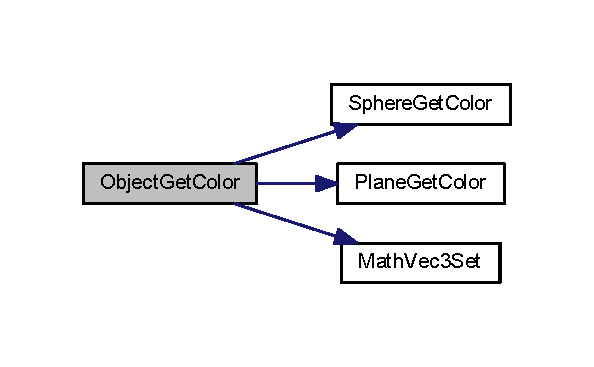
\includegraphics[width=285pt]{rayobject_8h_a85b5e2864495dc8d6fb2089fd6ec183e_cgraph}
\end{center}
\end{figure}




Here is the caller graph for this function\+:\nopagebreak
\begin{figure}[H]
\begin{center}
\leavevmode
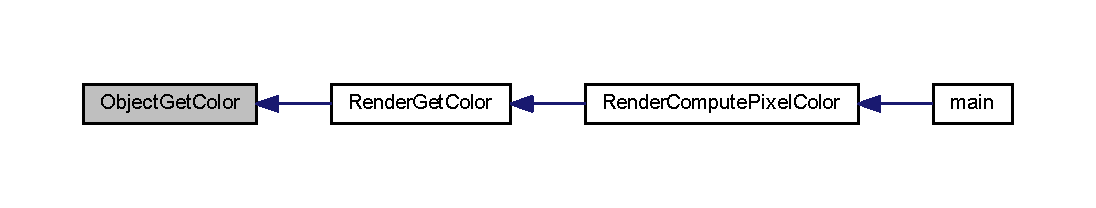
\includegraphics[width=350pt]{rayobject_8h_a85b5e2864495dc8d6fb2089fd6ec183e_icgraph}
\end{center}
\end{figure}


\index{rayobject.\+h@{rayobject.\+h}!Object\+Get\+Normal@{Object\+Get\+Normal}}
\index{Object\+Get\+Normal@{Object\+Get\+Normal}!rayobject.\+h@{rayobject.\+h}}
\subsubsection[{\texorpdfstring{Object\+Get\+Normal(int type, int idx, vec3\+\_\+t p, vec3\+\_\+t inside)}{ObjectGetNormal(int type, int idx, vec3_t p, vec3_t inside)}}]{\setlength{\rightskip}{0pt plus 5cm}{\bf vec3\+\_\+t} Object\+Get\+Normal (
\begin{DoxyParamCaption}
\item[{int}]{type, }
\item[{int}]{idx, }
\item[{{\bf vec3\+\_\+t}}]{p, }
\item[{{\bf vec3\+\_\+t}}]{inside}
\end{DoxyParamCaption}
)}\hypertarget{rayobject_8h_ad5b91bc5eba77d5f29d82147b63bd30f}{}\label{rayobject_8h_ad5b91bc5eba77d5f29d82147b63bd30f}


Get an object normal. 


\begin{DoxyParams}{Parameters}
{\em type} & Object type (O\+B\+J\+E\+C\+T\+\_\+\+T\+Y\+P\+E\+\_\+\+S\+P\+H\+E\+RE or O\+B\+J\+E\+C\+T\+\_\+\+T\+Y\+P\+E\+\_\+\+P\+L\+A\+NE) \\
\hline
{\em idx} & Object identifier \\
\hline
{\em p} & Intersection point position \\
\hline
{\em inside} & origin (applies for planes only) \\
\hline
\end{DoxyParams}
\begin{DoxyReturn}{Returns}
Object normal 
\end{DoxyReturn}


Definition at line 20 of file rayobject.\+c.



Here is the call graph for this function\+:\nopagebreak
\begin{figure}[H]
\begin{center}
\leavevmode
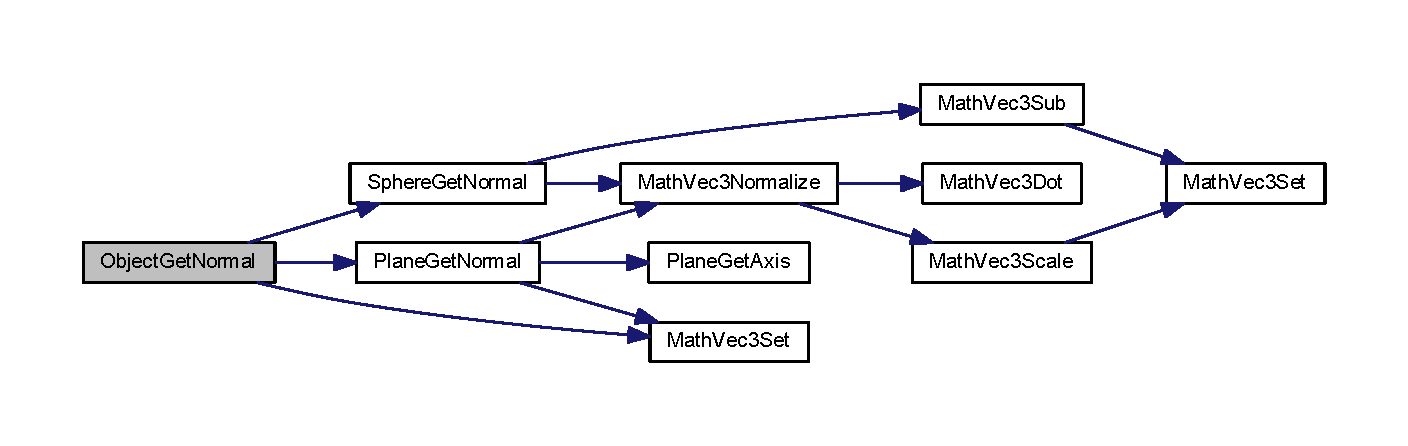
\includegraphics[width=350pt]{rayobject_8h_ad5b91bc5eba77d5f29d82147b63bd30f_cgraph}
\end{center}
\end{figure}




Here is the caller graph for this function\+:\nopagebreak
\begin{figure}[H]
\begin{center}
\leavevmode
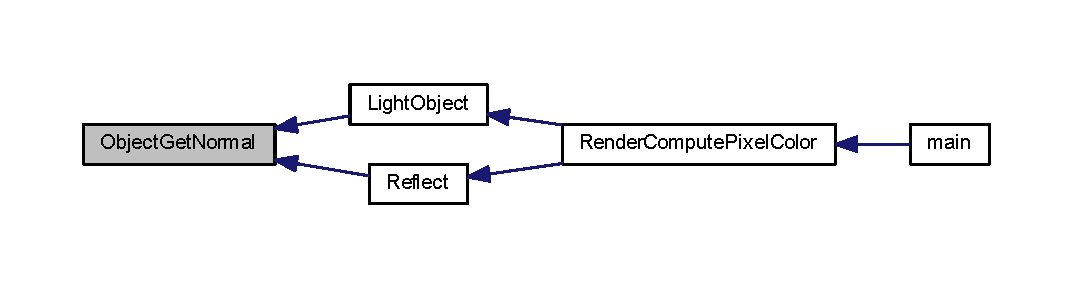
\includegraphics[width=350pt]{rayobject_8h_ad5b91bc5eba77d5f29d82147b63bd30f_icgraph}
\end{center}
\end{figure}


\index{rayobject.\+h@{rayobject.\+h}!Object\+Get\+Number\+By\+Type@{Object\+Get\+Number\+By\+Type}}
\index{Object\+Get\+Number\+By\+Type@{Object\+Get\+Number\+By\+Type}!rayobject.\+h@{rayobject.\+h}}
\subsubsection[{\texorpdfstring{Object\+Get\+Number\+By\+Type(int type)}{ObjectGetNumberByType(int type)}}]{\setlength{\rightskip}{0pt plus 5cm}{\bf u32\+\_\+t} Object\+Get\+Number\+By\+Type (
\begin{DoxyParamCaption}
\item[{int}]{type}
\end{DoxyParamCaption}
)}\hypertarget{rayobject_8h_a07163c81c5ae4159950c28fcaa835fc2}{}\label{rayobject_8h_a07163c81c5ae4159950c28fcaa835fc2}


Get the number of objects given a type. 


\begin{DoxyParams}{Parameters}
{\em type} & Object type (O\+B\+J\+E\+C\+T\+\_\+\+T\+Y\+P\+E\+\_\+\+S\+P\+H\+E\+RE or O\+B\+J\+E\+C\+T\+\_\+\+T\+Y\+P\+E\+\_\+\+P\+L\+A\+NE) \\
\hline
\end{DoxyParams}
\begin{DoxyReturn}{Returns}
Number of objects (by type) 
\end{DoxyReturn}


Definition at line 11 of file rayobject.\+c.



Here is the call graph for this function\+:\nopagebreak
\begin{figure}[H]
\begin{center}
\leavevmode
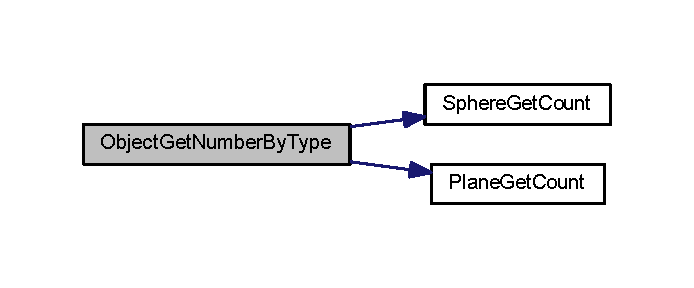
\includegraphics[width=333pt]{rayobject_8h_a07163c81c5ae4159950c28fcaa835fc2_cgraph}
\end{center}
\end{figure}




Here is the caller graph for this function\+:\nopagebreak
\begin{figure}[H]
\begin{center}
\leavevmode
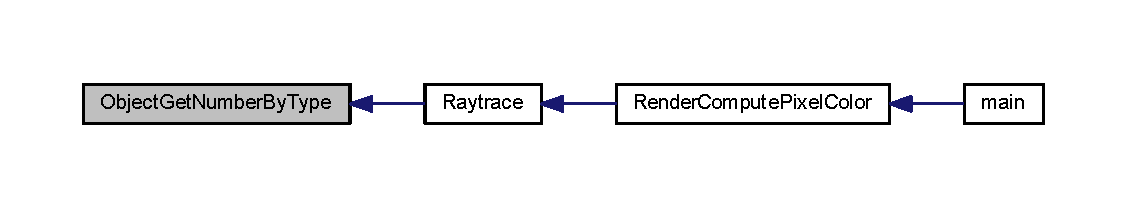
\includegraphics[width=350pt]{rayobject_8h_a07163c81c5ae4159950c28fcaa835fc2_icgraph}
\end{center}
\end{figure}



\hypertarget{rayplane_8h}{}\section{Includes/rayplane.h File Reference}
\label{rayplane_8h}\index{Includes/rayplane.\+h@{Includes/rayplane.\+h}}


Raytracer plane object.  


{\ttfamily \#include \char`\"{}raymath.\+h\char`\"{}}\\*
Include dependency graph for rayplane.\+h\+:\nopagebreak
\begin{figure}[H]
\begin{center}
\leavevmode
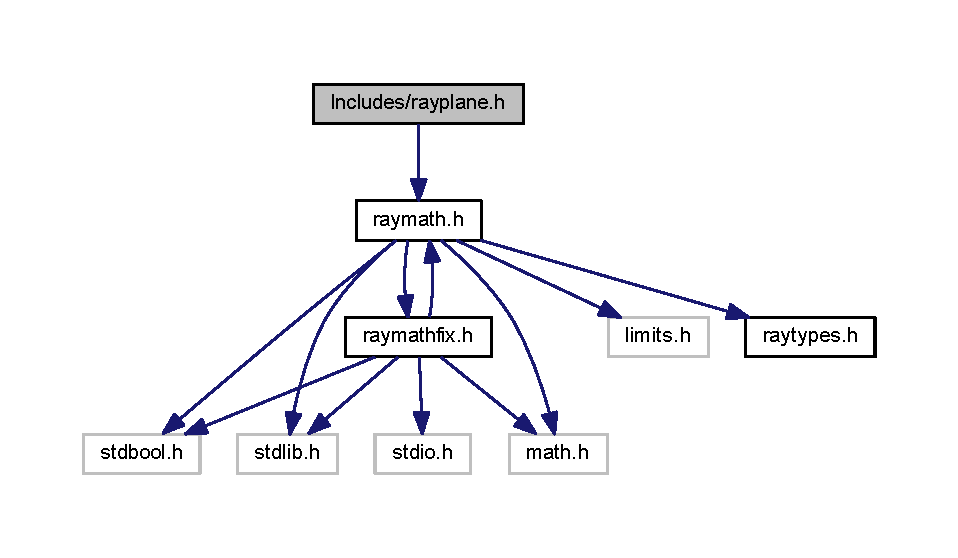
\includegraphics[width=350pt]{rayplane_8h__incl}
\end{center}
\end{figure}
This graph shows which files directly or indirectly include this file\+:
\nopagebreak
\begin{figure}[H]
\begin{center}
\leavevmode
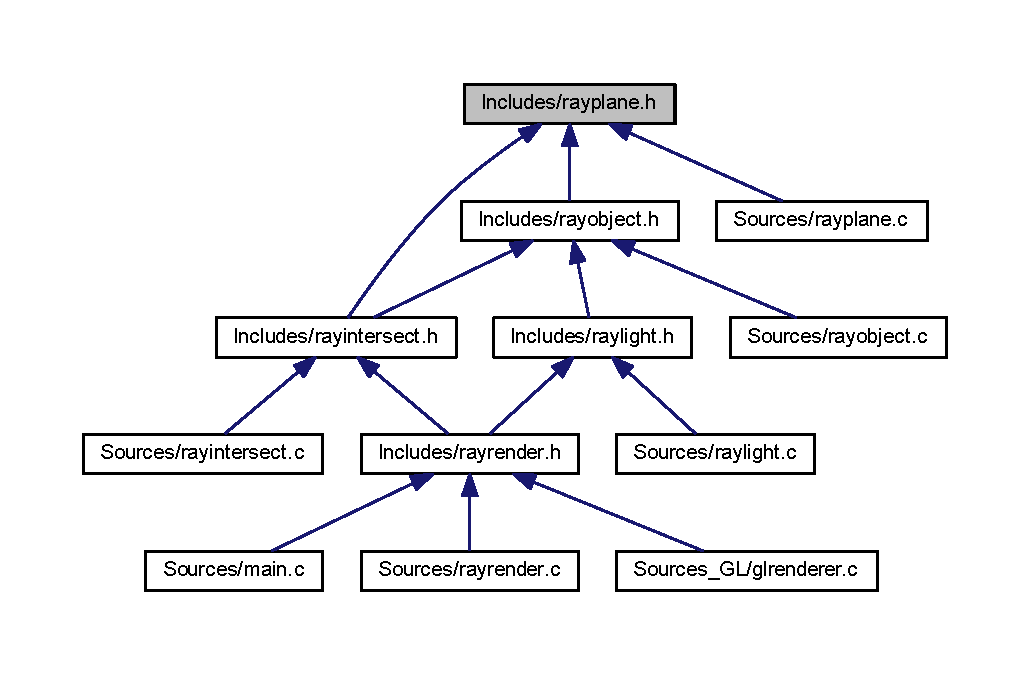
\includegraphics[width=350pt]{rayplane_8h__dep__incl}
\end{center}
\end{figure}
\subsection*{Data Structures}
\begin{DoxyCompactItemize}
\item 
struct \hyperlink{structplane}{plane}
\end{DoxyCompactItemize}
\subsection*{Macros}
\begin{DoxyCompactItemize}
\item 
\#define \hyperlink{rayplane_8h_a4269718bae6e29c6059d666ec76df24b}{M\+A\+X\+\_\+\+P\+L\+A\+N\+ES}~16
\begin{DoxyCompactList}\small\item\em Maximum number of planes in the current scene. \end{DoxyCompactList}\end{DoxyCompactItemize}
\subsection*{Typedefs}
\begin{DoxyCompactItemize}
\item 
typedef struct \hyperlink{structplane}{plane} \hyperlink{rayplane_8h_af6157b036db4c4437002ed82ab68cd3a}{plane\+\_\+t}
\begin{DoxyCompactList}\small\item\em A Structure to represent an intersection data. \end{DoxyCompactList}\end{DoxyCompactItemize}
\subsection*{Functions}
\begin{DoxyCompactItemize}
\item 
\hyperlink{raytypes_8h_a0c0a490ab7fa397be6c764a935cc5ea4}{u32\+\_\+t} \hyperlink{rayplane_8h_a2496f928d63b409b68e1276c0fd9bd56}{Plane\+Add} ()
\begin{DoxyCompactList}\small\item\em Add a plane to the current scene. \end{DoxyCompactList}\item 
\hyperlink{raytypes_8h_a0c0a490ab7fa397be6c764a935cc5ea4}{u32\+\_\+t} \hyperlink{rayplane_8h_ae013daff4214176716319374caa20a6d}{Plane\+Get\+Count} ()
\begin{DoxyCompactList}\small\item\em Return the total number of planes in the current scene. \end{DoxyCompactList}\item 
void \hyperlink{rayplane_8h_abb59de43588ed0617065276581ef4688}{Plane\+Set} (int idx, \hyperlink{raymath_8h_aa97c1f529dc5a11a78758184c84a39c9}{number} axis, \hyperlink{raymath_8h_aa97c1f529dc5a11a78758184c84a39c9}{number} dist, \hyperlink{raymath_8h_afb3684d7701a8417d1a52fd94c84457c}{vec3\+\_\+t} color)
\begin{DoxyCompactList}\small\item\em Set a plane axis, its distance to camera and its color. \end{DoxyCompactList}\item 
int \hyperlink{rayplane_8h_ac2e10806dc95ee948ebd52bd20788511}{Plane\+Get\+Axis} (int idx)
\begin{DoxyCompactList}\small\item\em Get a plane axis. \end{DoxyCompactList}\item 
\hyperlink{raymath_8h_aa97c1f529dc5a11a78758184c84a39c9}{number} \hyperlink{rayplane_8h_ad19ab75282017457d843661c97f2e980}{Plane\+Get\+Distance} (int idx)
\begin{DoxyCompactList}\small\item\em Get a plane distance from camera. \end{DoxyCompactList}\item 
\hyperlink{raymath_8h_afb3684d7701a8417d1a52fd94c84457c}{vec3\+\_\+t} \hyperlink{rayplane_8h_a24796f2ce83ad2b6c54b7e128d2bfb79}{Plane\+Get\+Color} (int idx)
\begin{DoxyCompactList}\small\item\em Get a plane color. \end{DoxyCompactList}\item 
\hyperlink{raymath_8h_afb3684d7701a8417d1a52fd94c84457c}{vec3\+\_\+t} \hyperlink{rayplane_8h_a2d9da63f70736e7978942968a0752358}{Plane\+Get\+Normal} (int idx, \hyperlink{raymath_8h_afb3684d7701a8417d1a52fd94c84457c}{vec3\+\_\+t} o)
\begin{DoxyCompactList}\small\item\em Get a plane normal. \end{DoxyCompactList}\end{DoxyCompactItemize}


\subsection{Detailed Description}
Raytracer plane object. 

\begin{DoxyAuthor}{Author}
J. Crenne \& C. Leroux 
\end{DoxyAuthor}
\begin{DoxyVersion}{Version}
1.\+0 
\end{DoxyVersion}
\begin{DoxyDate}{Date}
February 2016 
\end{DoxyDate}


\subsection{Macro Definition Documentation}
\index{rayplane.\+h@{rayplane.\+h}!M\+A\+X\+\_\+\+P\+L\+A\+N\+ES@{M\+A\+X\+\_\+\+P\+L\+A\+N\+ES}}
\index{M\+A\+X\+\_\+\+P\+L\+A\+N\+ES@{M\+A\+X\+\_\+\+P\+L\+A\+N\+ES}!rayplane.\+h@{rayplane.\+h}}
\subsubsection[{\texorpdfstring{M\+A\+X\+\_\+\+P\+L\+A\+N\+ES}{MAX_PLANES}}]{\setlength{\rightskip}{0pt plus 5cm}\#define M\+A\+X\+\_\+\+P\+L\+A\+N\+ES~16}\hypertarget{rayplane_8h_a4269718bae6e29c6059d666ec76df24b}{}\label{rayplane_8h_a4269718bae6e29c6059d666ec76df24b}


Maximum number of planes in the current scene. 



Definition at line 18 of file rayplane.\+h.



\subsection{Typedef Documentation}
\index{rayplane.\+h@{rayplane.\+h}!plane\+\_\+t@{plane\+\_\+t}}
\index{plane\+\_\+t@{plane\+\_\+t}!rayplane.\+h@{rayplane.\+h}}
\subsubsection[{\texorpdfstring{plane\+\_\+t}{plane_t}}]{\setlength{\rightskip}{0pt plus 5cm}{\bf plane\+\_\+t}}\hypertarget{rayplane_8h_af6157b036db4c4437002ed82ab68cd3a}{}\label{rayplane_8h_af6157b036db4c4437002ed82ab68cd3a}


A Structure to represent an intersection data. 

A Structure to represent a plane. 

\subsection{Function Documentation}
\index{rayplane.\+h@{rayplane.\+h}!Plane\+Add@{Plane\+Add}}
\index{Plane\+Add@{Plane\+Add}!rayplane.\+h@{rayplane.\+h}}
\subsubsection[{\texorpdfstring{Plane\+Add()}{PlaneAdd()}}]{\setlength{\rightskip}{0pt plus 5cm}{\bf u32\+\_\+t} Plane\+Add (
\begin{DoxyParamCaption}
{}
\end{DoxyParamCaption}
)}\hypertarget{rayplane_8h_a2496f928d63b409b68e1276c0fd9bd56}{}\label{rayplane_8h_a2496f928d63b409b68e1276c0fd9bd56}


Add a plane to the current scene. 

\begin{DoxyReturn}{Returns}
a unique plane identifier 
\end{DoxyReturn}


Definition at line 14 of file rayplane.\+c.



Here is the caller graph for this function\+:\nopagebreak
\begin{figure}[H]
\begin{center}
\leavevmode
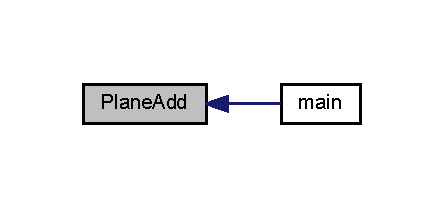
\includegraphics[width=213pt]{rayplane_8h_a2496f928d63b409b68e1276c0fd9bd56_icgraph}
\end{center}
\end{figure}


\index{rayplane.\+h@{rayplane.\+h}!Plane\+Get\+Axis@{Plane\+Get\+Axis}}
\index{Plane\+Get\+Axis@{Plane\+Get\+Axis}!rayplane.\+h@{rayplane.\+h}}
\subsubsection[{\texorpdfstring{Plane\+Get\+Axis(int idx)}{PlaneGetAxis(int idx)}}]{\setlength{\rightskip}{0pt plus 5cm}{\bf number} Plane\+Get\+Axis (
\begin{DoxyParamCaption}
\item[{int}]{idx}
\end{DoxyParamCaption}
)}\hypertarget{rayplane_8h_ac2e10806dc95ee948ebd52bd20788511}{}\label{rayplane_8h_ac2e10806dc95ee948ebd52bd20788511}


Get a plane axis. 


\begin{DoxyParams}{Parameters}
{\em idx} & Plane identifier \\
\hline
\end{DoxyParams}
\begin{DoxyReturn}{Returns}
Plane axis 
\end{DoxyReturn}


Definition at line 32 of file rayplane.\+c.



Here is the caller graph for this function\+:\nopagebreak
\begin{figure}[H]
\begin{center}
\leavevmode
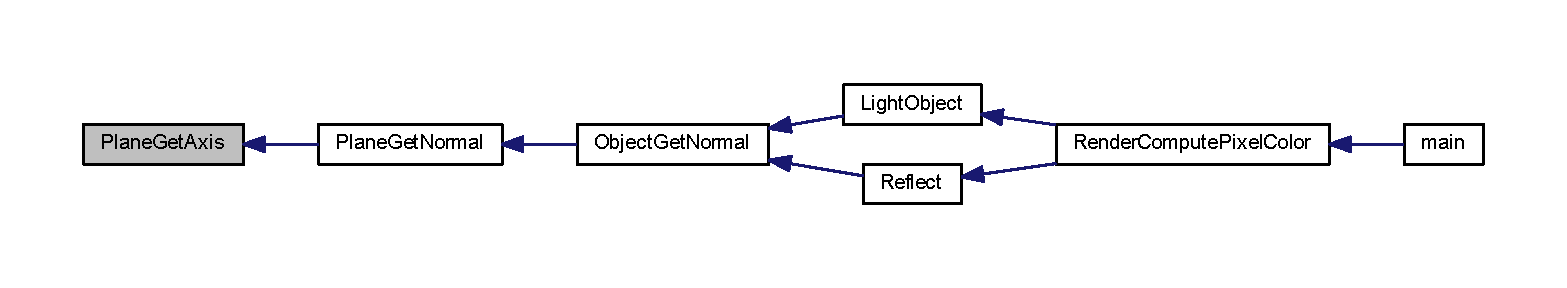
\includegraphics[width=350pt]{rayplane_8h_ac2e10806dc95ee948ebd52bd20788511_icgraph}
\end{center}
\end{figure}


\index{rayplane.\+h@{rayplane.\+h}!Plane\+Get\+Color@{Plane\+Get\+Color}}
\index{Plane\+Get\+Color@{Plane\+Get\+Color}!rayplane.\+h@{rayplane.\+h}}
\subsubsection[{\texorpdfstring{Plane\+Get\+Color(int idx)}{PlaneGetColor(int idx)}}]{\setlength{\rightskip}{0pt plus 5cm}{\bf vec3\+\_\+t} Plane\+Get\+Color (
\begin{DoxyParamCaption}
\item[{int}]{idx}
\end{DoxyParamCaption}
)}\hypertarget{rayplane_8h_a24796f2ce83ad2b6c54b7e128d2bfb79}{}\label{rayplane_8h_a24796f2ce83ad2b6c54b7e128d2bfb79}


Get a plane color. 


\begin{DoxyParams}{Parameters}
{\em idx} & Plane identifier \\
\hline
\end{DoxyParams}
\begin{DoxyReturn}{Returns}
Plane color 
\end{DoxyReturn}


Definition at line 36 of file rayplane.\+c.



Here is the caller graph for this function\+:\nopagebreak
\begin{figure}[H]
\begin{center}
\leavevmode
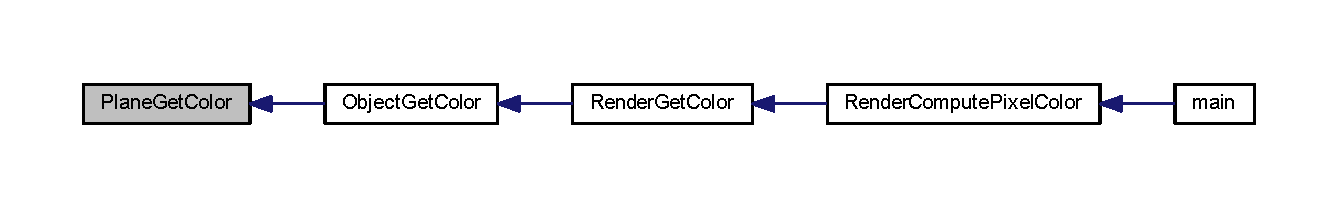
\includegraphics[width=350pt]{rayplane_8h_a24796f2ce83ad2b6c54b7e128d2bfb79_icgraph}
\end{center}
\end{figure}


\index{rayplane.\+h@{rayplane.\+h}!Plane\+Get\+Count@{Plane\+Get\+Count}}
\index{Plane\+Get\+Count@{Plane\+Get\+Count}!rayplane.\+h@{rayplane.\+h}}
\subsubsection[{\texorpdfstring{Plane\+Get\+Count()}{PlaneGetCount()}}]{\setlength{\rightskip}{0pt plus 5cm}{\bf u32\+\_\+t} Plane\+Get\+Count (
\begin{DoxyParamCaption}
{}
\end{DoxyParamCaption}
)}\hypertarget{rayplane_8h_ae013daff4214176716319374caa20a6d}{}\label{rayplane_8h_ae013daff4214176716319374caa20a6d}


Return the total number of planes in the current scene. 

\begin{DoxyReturn}{Returns}
Number of planes 
\end{DoxyReturn}


Definition at line 18 of file rayplane.\+c.



Here is the caller graph for this function\+:\nopagebreak
\begin{figure}[H]
\begin{center}
\leavevmode
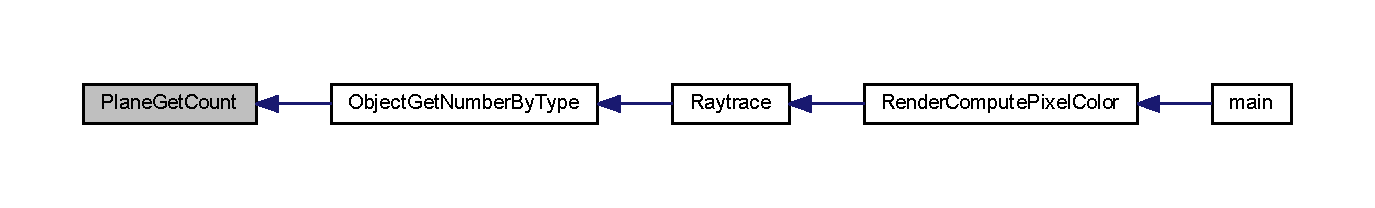
\includegraphics[width=350pt]{rayplane_8h_ae013daff4214176716319374caa20a6d_icgraph}
\end{center}
\end{figure}


\index{rayplane.\+h@{rayplane.\+h}!Plane\+Get\+Distance@{Plane\+Get\+Distance}}
\index{Plane\+Get\+Distance@{Plane\+Get\+Distance}!rayplane.\+h@{rayplane.\+h}}
\subsubsection[{\texorpdfstring{Plane\+Get\+Distance(int idx)}{PlaneGetDistance(int idx)}}]{\setlength{\rightskip}{0pt plus 5cm}{\bf number} Plane\+Get\+Distance (
\begin{DoxyParamCaption}
\item[{int}]{idx}
\end{DoxyParamCaption}
)}\hypertarget{rayplane_8h_ad19ab75282017457d843661c97f2e980}{}\label{rayplane_8h_ad19ab75282017457d843661c97f2e980}


Get a plane distance from camera. 


\begin{DoxyParams}{Parameters}
{\em idx} & Plane identifier \\
\hline
\end{DoxyParams}


Definition at line 28 of file rayplane.\+c.

\index{rayplane.\+h@{rayplane.\+h}!Plane\+Get\+Normal@{Plane\+Get\+Normal}}
\index{Plane\+Get\+Normal@{Plane\+Get\+Normal}!rayplane.\+h@{rayplane.\+h}}
\subsubsection[{\texorpdfstring{Plane\+Get\+Normal(int idx, vec3\+\_\+t o)}{PlaneGetNormal(int idx, vec3_t o)}}]{\setlength{\rightskip}{0pt plus 5cm}{\bf vec3\+\_\+t} Plane\+Get\+Normal (
\begin{DoxyParamCaption}
\item[{int}]{idx, }
\item[{{\bf vec3\+\_\+t}}]{o}
\end{DoxyParamCaption}
)}\hypertarget{rayplane_8h_a2d9da63f70736e7978942968a0752358}{}\label{rayplane_8h_a2d9da63f70736e7978942968a0752358}


Get a plane normal. 


\begin{DoxyParams}{Parameters}
{\em idx} & Plane identifier \\
\hline
{\em o} & origin \\
\hline
\end{DoxyParams}
\begin{DoxyReturn}{Returns}
Plane normal 
\end{DoxyReturn}


Definition at line 40 of file rayplane.\+c.



Here is the call graph for this function\+:\nopagebreak
\begin{figure}[H]
\begin{center}
\leavevmode
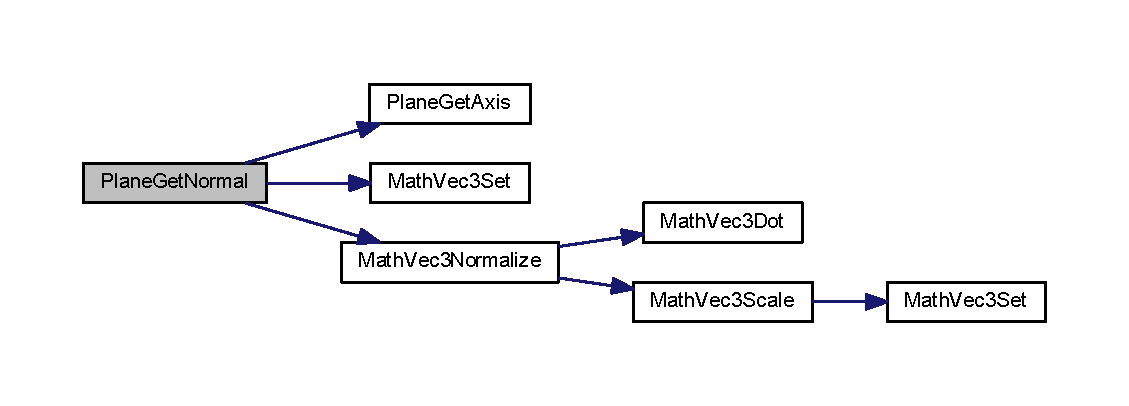
\includegraphics[width=350pt]{rayplane_8h_a2d9da63f70736e7978942968a0752358_cgraph}
\end{center}
\end{figure}




Here is the caller graph for this function\+:\nopagebreak
\begin{figure}[H]
\begin{center}
\leavevmode
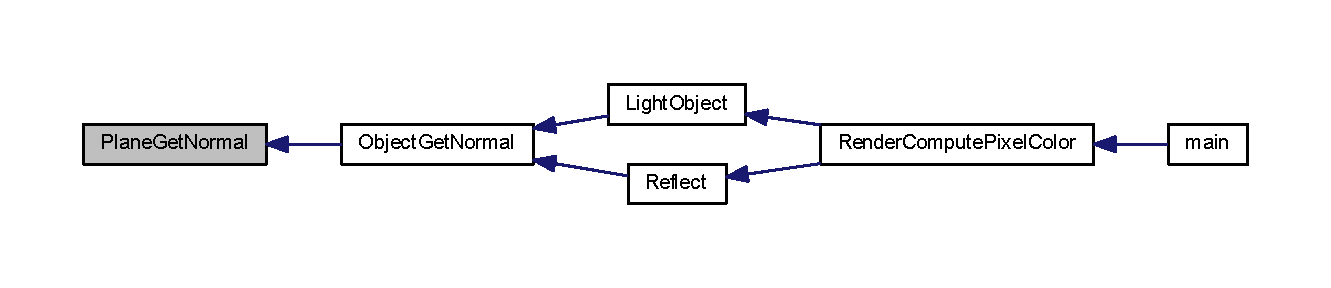
\includegraphics[width=350pt]{rayplane_8h_a2d9da63f70736e7978942968a0752358_icgraph}
\end{center}
\end{figure}


\index{rayplane.\+h@{rayplane.\+h}!Plane\+Set@{Plane\+Set}}
\index{Plane\+Set@{Plane\+Set}!rayplane.\+h@{rayplane.\+h}}
\subsubsection[{\texorpdfstring{Plane\+Set(int idx, number axis, number dist, vec3\+\_\+t color)}{PlaneSet(int idx, number axis, number dist, vec3_t color)}}]{\setlength{\rightskip}{0pt plus 5cm}void Plane\+Set (
\begin{DoxyParamCaption}
\item[{int}]{idx, }
\item[{{\bf number}}]{axis, }
\item[{{\bf number}}]{dist, }
\item[{{\bf vec3\+\_\+t}}]{color}
\end{DoxyParamCaption}
)}\hypertarget{rayplane_8h_abb59de43588ed0617065276581ef4688}{}\label{rayplane_8h_abb59de43588ed0617065276581ef4688}


Set a plane axis, its distance to camera and its color. 


\begin{DoxyParams}{Parameters}
{\em idx} & Plane identifier \\
\hline
{\em axis} & Plane axis \\
\hline
{\em dist} & Plane distance to camera \\
\hline
{\em color} & Plane color \\
\hline
\end{DoxyParams}


Definition at line 22 of file rayplane.\+c.



Here is the caller graph for this function\+:\nopagebreak
\begin{figure}[H]
\begin{center}
\leavevmode
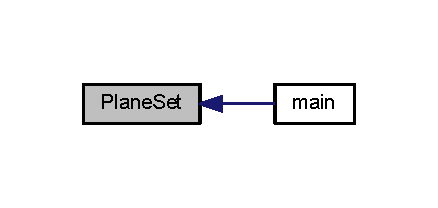
\includegraphics[width=210pt]{rayplane_8h_abb59de43588ed0617065276581ef4688_icgraph}
\end{center}
\end{figure}



\hypertarget{rayrender_8h}{}\section{Includes/rayrender.h File Reference}
\label{rayrender_8h}\index{Includes/rayrender.\+h@{Includes/rayrender.\+h}}


Raytracer scene rendering.  


{\ttfamily \#include $<$stdio.\+h$>$}\\*
{\ttfamily \#include $<$stdbool.\+h$>$}\\*
{\ttfamily \#include $<$float.\+h$>$}\\*
{\ttfamily \#include \char`\"{}raymath.\+h\char`\"{}}\\*
{\ttfamily \#include \char`\"{}rayintersect.\+h\char`\"{}}\\*
{\ttfamily \#include \char`\"{}raylight.\+h\char`\"{}}\\*
Include dependency graph for rayrender.\+h\+:\nopagebreak
\begin{figure}[H]
\begin{center}
\leavevmode
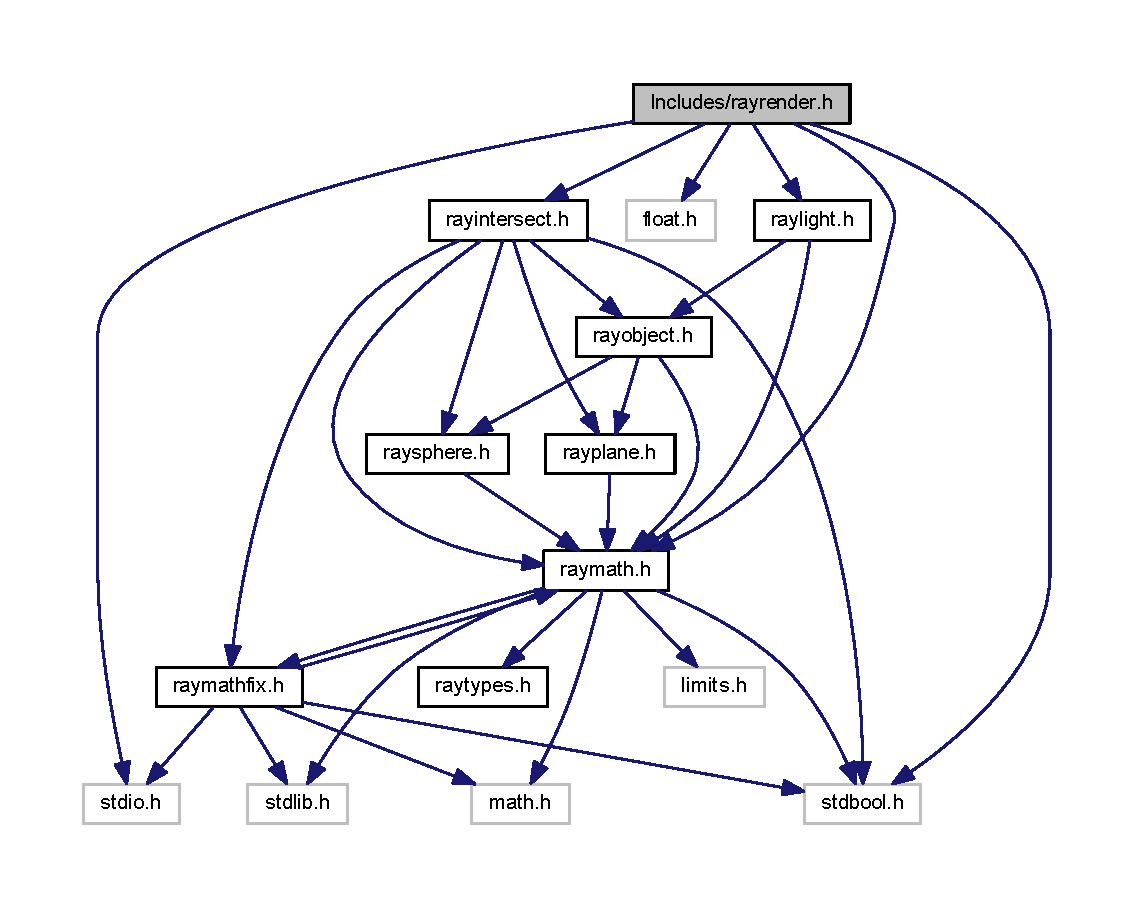
\includegraphics[width=350pt]{rayrender_8h__incl}
\end{center}
\end{figure}
This graph shows which files directly or indirectly include this file\+:
\nopagebreak
\begin{figure}[H]
\begin{center}
\leavevmode
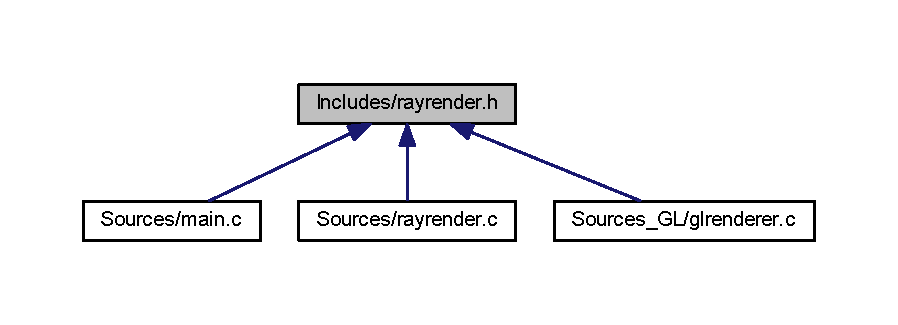
\includegraphics[width=350pt]{rayrender_8h__dep__incl}
\end{center}
\end{figure}
\subsection*{Macros}
\begin{DoxyCompactItemize}
\item 
\#define \hyperlink{rayrender_8h_aee75d0130ade17390942add50c7eac24}{S\+I\+Z\+E\+\_\+\+I\+MG}~4
\begin{DoxyCompactList}\small\item\em Size of image output. \end{DoxyCompactList}\end{DoxyCompactItemize}
\subsection*{Functions}
\begin{DoxyCompactItemize}
\item 
void \hyperlink{rayrender_8h_acc66fa75cd6a184f46af374fc8004d2c}{Render\+Setup} (\hyperlink{raymath_8h_afb3684d7701a8417d1a52fd94c84457c}{vec3\+\_\+t} l, \hyperlink{raymath_8h_aa97c1f529dc5a11a78758184c84a39c9}{number} ambient, \hyperlink{raytypes_8h_a0c0a490ab7fa397be6c764a935cc5ea4}{u32\+\_\+t} maxr)
\begin{DoxyCompactList}\small\item\em Setup the render context. \end{DoxyCompactList}\item 
void \hyperlink{rayrender_8h_afd5f3dfa0756d697a86e818cdbf49a56}{Render\+Reset} ()
\begin{DoxyCompactList}\small\item\em Reset the render context. \end{DoxyCompactList}\item 
void \hyperlink{rayrender_8h_a436830dff9fbce05c931c5a6d8d5366d}{Render} ()
\begin{DoxyCompactList}\small\item\em Render the current scene. \end{DoxyCompactList}\item 
\hyperlink{raymath_8h_afb3684d7701a8417d1a52fd94c84457c}{vec3\+\_\+t} \hyperlink{rayrender_8h_a5cbf8abb7997119c522463eb111b2a3e}{Render\+Compute\+Pixel\+Color} (\hyperlink{raytypes_8h_a0c0a490ab7fa397be6c764a935cc5ea4}{u32\+\_\+t} size, \hyperlink{raymath_8h_aa97c1f529dc5a11a78758184c84a39c9}{number} x, \hyperlink{raymath_8h_aa97c1f529dc5a11a78758184c84a39c9}{number} y)
\begin{DoxyCompactList}\small\item\em Render the current scene. \end{DoxyCompactList}\end{DoxyCompactItemize}


\subsection{Detailed Description}
Raytracer scene rendering. 

\begin{DoxyAuthor}{Author}
J. Crenne \& C. Leroux 
\end{DoxyAuthor}
\begin{DoxyVersion}{Version}
1.\+0 
\end{DoxyVersion}
\begin{DoxyDate}{Date}
February 2016 
\end{DoxyDate}


\subsection{Macro Definition Documentation}
\index{rayrender.\+h@{rayrender.\+h}!S\+I\+Z\+E\+\_\+\+I\+MG@{S\+I\+Z\+E\+\_\+\+I\+MG}}
\index{S\+I\+Z\+E\+\_\+\+I\+MG@{S\+I\+Z\+E\+\_\+\+I\+MG}!rayrender.\+h@{rayrender.\+h}}
\subsubsection[{\texorpdfstring{S\+I\+Z\+E\+\_\+\+I\+MG}{SIZE_IMG}}]{\setlength{\rightskip}{0pt plus 5cm}\#define S\+I\+Z\+E\+\_\+\+I\+MG~4}\hypertarget{rayrender_8h_aee75d0130ade17390942add50c7eac24}{}\label{rayrender_8h_aee75d0130ade17390942add50c7eac24}


Size of image output. 



Definition at line 25 of file rayrender.\+h.



\subsection{Function Documentation}
\index{rayrender.\+h@{rayrender.\+h}!Render@{Render}}
\index{Render@{Render}!rayrender.\+h@{rayrender.\+h}}
\subsubsection[{\texorpdfstring{Render()}{Render()}}]{\setlength{\rightskip}{0pt plus 5cm}void Render (
\begin{DoxyParamCaption}
{}
\end{DoxyParamCaption}
)}\hypertarget{rayrender_8h_a436830dff9fbce05c931c5a6d8d5366d}{}\label{rayrender_8h_a436830dff9fbce05c931c5a6d8d5366d}


Render the current scene. 



Here is the caller graph for this function\+:\nopagebreak
\begin{figure}[H]
\begin{center}
\leavevmode
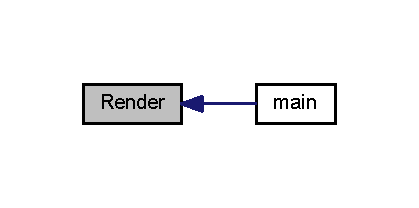
\includegraphics[width=201pt]{rayrender_8h_a436830dff9fbce05c931c5a6d8d5366d_icgraph}
\end{center}
\end{figure}


\index{rayrender.\+h@{rayrender.\+h}!Render\+Compute\+Pixel\+Color@{Render\+Compute\+Pixel\+Color}}
\index{Render\+Compute\+Pixel\+Color@{Render\+Compute\+Pixel\+Color}!rayrender.\+h@{rayrender.\+h}}
\subsubsection[{\texorpdfstring{Render\+Compute\+Pixel\+Color(u32\+\_\+t size, number x, number y)}{RenderComputePixelColor(u32_t size, number x, number y)}}]{\setlength{\rightskip}{0pt plus 5cm}{\bf vec3\+\_\+t} Render\+Compute\+Pixel\+Color (
\begin{DoxyParamCaption}
\item[{{\bf u32\+\_\+t}}]{size, }
\item[{{\bf number}}]{x, }
\item[{{\bf number}}]{y}
\end{DoxyParamCaption}
)}\hypertarget{rayrender_8h_a5cbf8abb7997119c522463eb111b2a3e}{}\label{rayrender_8h_a5cbf8abb7997119c522463eb111b2a3e}


Render the current scene. 


\begin{DoxyParams}{Parameters}
{\em size} & Size of output \char`\"{}pixel\char`\"{} \\
\hline
{\em x} & Pixel x position \\
\hline
{\em y} & Pixel y position \\
\hline
\end{DoxyParams}
\begin{DoxyReturn}{Returns}
A 3D vector representing the computed pixel color 
\end{DoxyReturn}


Definition at line 76 of file rayrender.\+c.



Here is the call graph for this function\+:\nopagebreak
\begin{figure}[H]
\begin{center}
\leavevmode
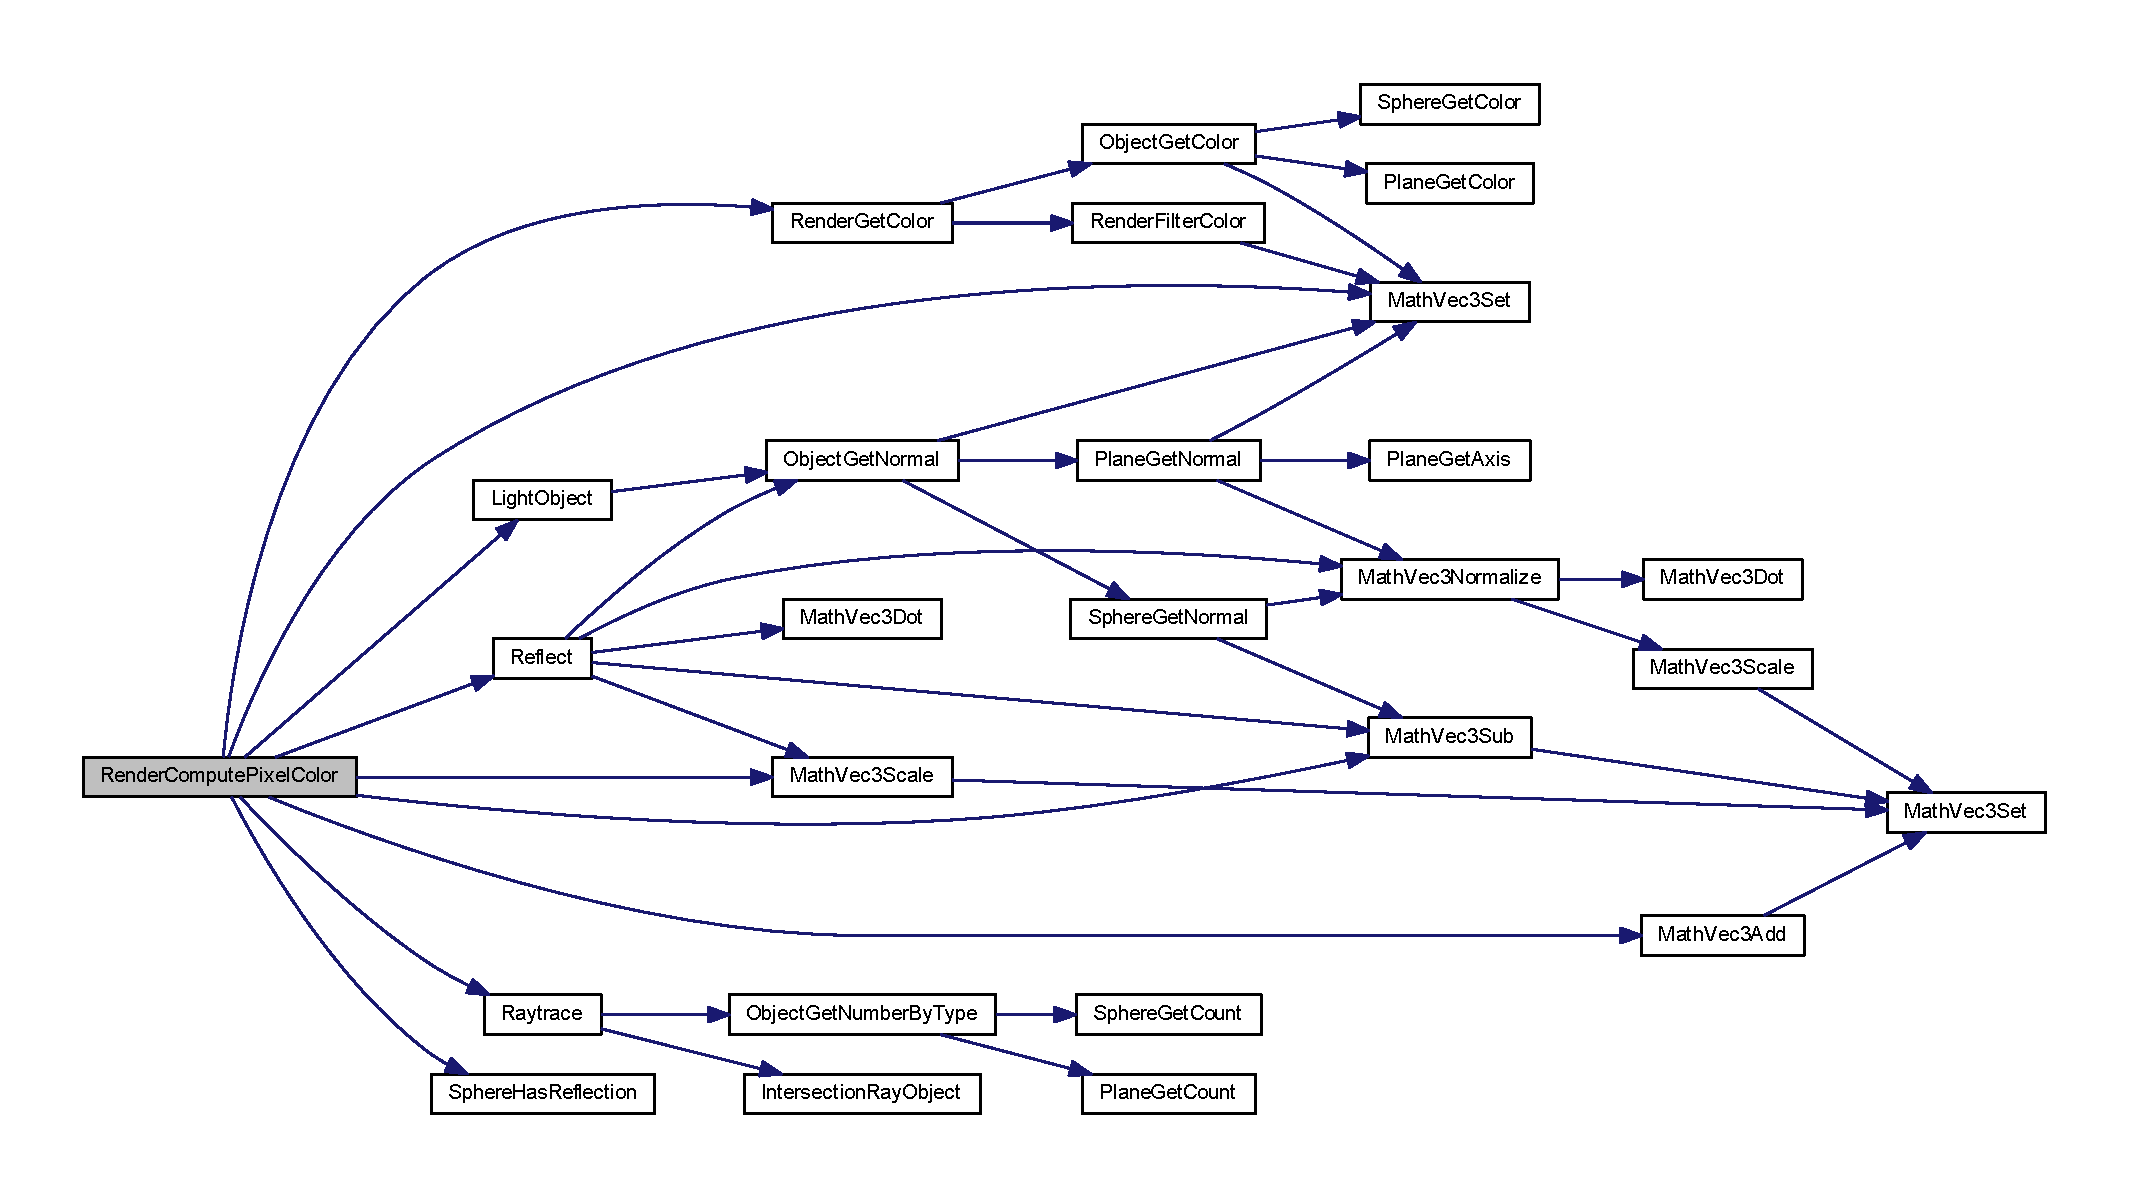
\includegraphics[width=350pt]{rayrender_8h_a5cbf8abb7997119c522463eb111b2a3e_cgraph}
\end{center}
\end{figure}




Here is the caller graph for this function\+:\nopagebreak
\begin{figure}[H]
\begin{center}
\leavevmode
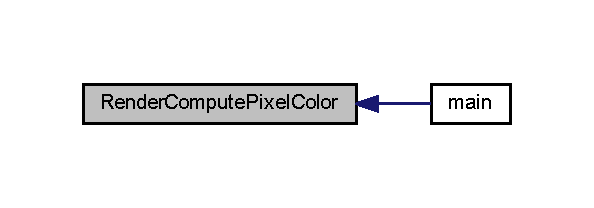
\includegraphics[width=285pt]{rayrender_8h_a5cbf8abb7997119c522463eb111b2a3e_icgraph}
\end{center}
\end{figure}


\index{rayrender.\+h@{rayrender.\+h}!Render\+Reset@{Render\+Reset}}
\index{Render\+Reset@{Render\+Reset}!rayrender.\+h@{rayrender.\+h}}
\subsubsection[{\texorpdfstring{Render\+Reset()}{RenderReset()}}]{\setlength{\rightskip}{0pt plus 5cm}void Render\+Reset (
\begin{DoxyParamCaption}
{}
\end{DoxyParamCaption}
)}\hypertarget{rayrender_8h_afd5f3dfa0756d697a86e818cdbf49a56}{}\label{rayrender_8h_afd5f3dfa0756d697a86e818cdbf49a56}


Reset the render context. 



Definition at line 23 of file rayrender.\+c.



Here is the caller graph for this function\+:\nopagebreak
\begin{figure}[H]
\begin{center}
\leavevmode
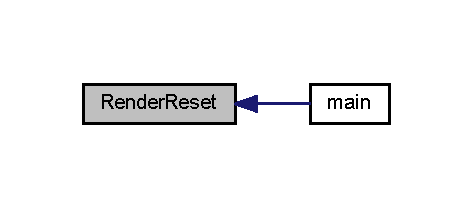
\includegraphics[width=227pt]{rayrender_8h_afd5f3dfa0756d697a86e818cdbf49a56_icgraph}
\end{center}
\end{figure}


\index{rayrender.\+h@{rayrender.\+h}!Render\+Setup@{Render\+Setup}}
\index{Render\+Setup@{Render\+Setup}!rayrender.\+h@{rayrender.\+h}}
\subsubsection[{\texorpdfstring{Render\+Setup(vec3\+\_\+t l, number ambient, u32\+\_\+t maxr)}{RenderSetup(vec3_t l, number ambient, u32_t maxr)}}]{\setlength{\rightskip}{0pt plus 5cm}void Render\+Setup (
\begin{DoxyParamCaption}
\item[{{\bf vec3\+\_\+t}}]{l, }
\item[{{\bf number}}]{ambient, }
\item[{{\bf u32\+\_\+t}}]{maxr}
\end{DoxyParamCaption}
)}\hypertarget{rayrender_8h_acc66fa75cd6a184f46af374fc8004d2c}{}\label{rayrender_8h_acc66fa75cd6a184f46af374fc8004d2c}


Setup the render context. 


\begin{DoxyParams}{Parameters}
{\em l} & Point light position \\
\hline
{\em ambient} & Ambient light multiplier factor \\
\hline
{\em maxr} & Maximum render resolution \\
\hline
\end{DoxyParams}


Definition at line 31 of file rayrender.\+c.



Here is the call graph for this function\+:\nopagebreak
\begin{figure}[H]
\begin{center}
\leavevmode
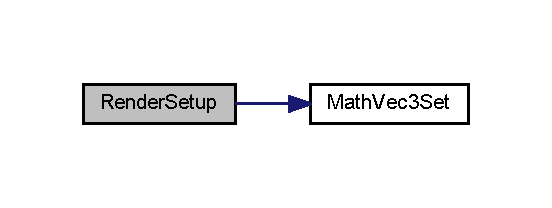
\includegraphics[width=265pt]{rayrender_8h_acc66fa75cd6a184f46af374fc8004d2c_cgraph}
\end{center}
\end{figure}




Here is the caller graph for this function\+:\nopagebreak
\begin{figure}[H]
\begin{center}
\leavevmode
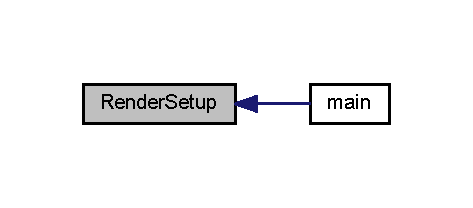
\includegraphics[width=227pt]{rayrender_8h_acc66fa75cd6a184f46af374fc8004d2c_icgraph}
\end{center}
\end{figure}



\hypertarget{raysphere_8h}{}\section{Includes/raysphere.h File Reference}
\label{raysphere_8h}\index{Includes/raysphere.\+h@{Includes/raysphere.\+h}}


Raytracer sphere object.  


{\ttfamily \#include \char`\"{}raymath.\+h\char`\"{}}\\*
Include dependency graph for raysphere.\+h\+:\nopagebreak
\begin{figure}[H]
\begin{center}
\leavevmode
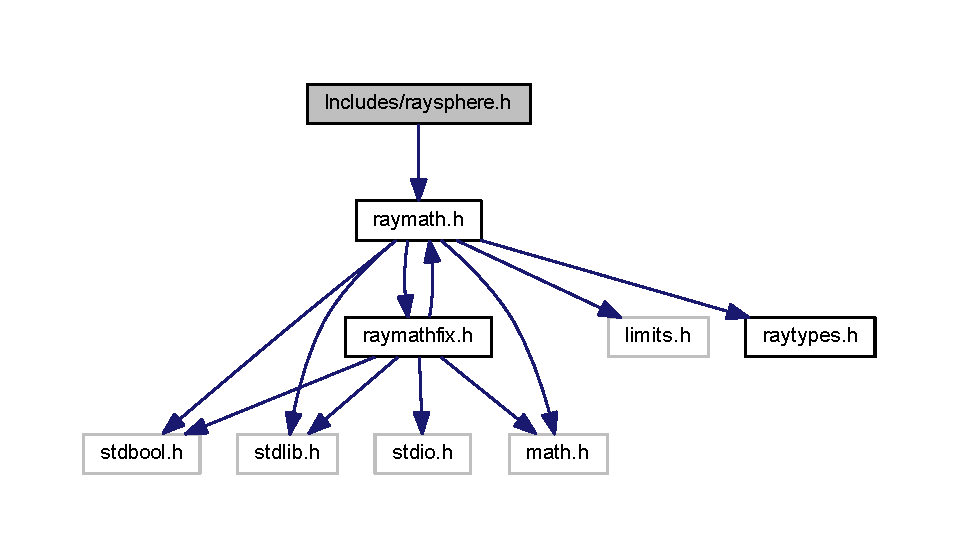
\includegraphics[width=350pt]{raysphere_8h__incl}
\end{center}
\end{figure}
This graph shows which files directly or indirectly include this file\+:
\nopagebreak
\begin{figure}[H]
\begin{center}
\leavevmode
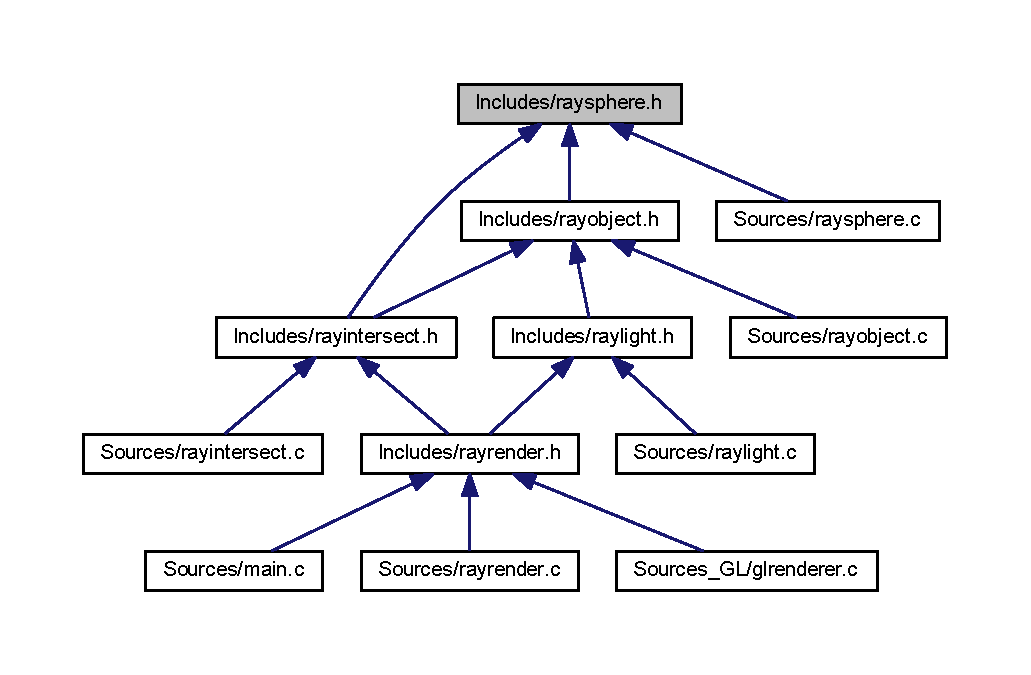
\includegraphics[width=350pt]{raysphere_8h__dep__incl}
\end{center}
\end{figure}
\subsection*{Data Structures}
\begin{DoxyCompactItemize}
\item 
struct \hyperlink{structsphere}{sphere}
\end{DoxyCompactItemize}
\subsection*{Macros}
\begin{DoxyCompactItemize}
\item 
\#define \hyperlink{raysphere_8h_a9266c2928d16a0ef8821cd280326a7ce}{M\+A\+X\+\_\+\+S\+P\+H\+E\+R\+ES}~16
\begin{DoxyCompactList}\small\item\em Maximum number of spheres in the current scene. \end{DoxyCompactList}\end{DoxyCompactItemize}
\subsection*{Typedefs}
\begin{DoxyCompactItemize}
\item 
typedef struct \hyperlink{structsphere}{sphere} \hyperlink{raysphere_8h_a29cdc396a1ac3ae3521d8a75a94f9909}{sphere\+\_\+t}
\begin{DoxyCompactList}\small\item\em A Structure to represent a sphere. \end{DoxyCompactList}\end{DoxyCompactItemize}
\subsection*{Functions}
\begin{DoxyCompactItemize}
\item 
\hyperlink{raytypes_8h_a0c0a490ab7fa397be6c764a935cc5ea4}{u32\+\_\+t} \hyperlink{raysphere_8h_a8302a4a5bcd3589308b809744019650d}{Sphere\+Add} ()
\begin{DoxyCompactList}\small\item\em Add a sphere to the current scene. \end{DoxyCompactList}\item 
\hyperlink{raytypes_8h_a0c0a490ab7fa397be6c764a935cc5ea4}{u32\+\_\+t} \hyperlink{raysphere_8h_ac10362606babe4fdfd1225750810046f}{Sphere\+Get\+Count} ()
\begin{DoxyCompactList}\small\item\em Return the total number of spheres in the current scene. \end{DoxyCompactList}\item 
void \hyperlink{raysphere_8h_a0c92d9eb3842a709c714c1f758187b29}{Sphere\+Set} (int idx, \hyperlink{raymath_8h_aa97c1f529dc5a11a78758184c84a39c9}{number} x, \hyperlink{raymath_8h_aa97c1f529dc5a11a78758184c84a39c9}{number} y, \hyperlink{raymath_8h_aa97c1f529dc5a11a78758184c84a39c9}{number} z, \hyperlink{raymath_8h_aa97c1f529dc5a11a78758184c84a39c9}{number} radius, \hyperlink{raymath_8h_afb3684d7701a8417d1a52fd94c84457c}{vec3\+\_\+t} color, bool reflect)
\begin{DoxyCompactList}\small\item\em Set a sphere position, its radius, its color and its reflection property. \end{DoxyCompactList}\item 
bool \hyperlink{raysphere_8h_aac374b086db079dd05b2b3c953abf4e8}{Sphere\+Has\+Reflection} (int idx)
\begin{DoxyCompactList}\small\item\em Get the reflection property of a sphere. \end{DoxyCompactList}\item 
\hyperlink{raymath_8h_afb3684d7701a8417d1a52fd94c84457c}{vec3\+\_\+t} \hyperlink{raysphere_8h_a1390f345c99ed67d84f05224e398a809}{Sphere\+Get\+Position} (int idx)
\begin{DoxyCompactList}\small\item\em Get the position of a sphere in the current scene. \end{DoxyCompactList}\item 
\hyperlink{raymath_8h_aa97c1f529dc5a11a78758184c84a39c9}{number} \hyperlink{raysphere_8h_a6a36d9c97c2630d8a078d3bc88b85d96}{Sphere\+Get\+Radius} (int idx)
\begin{DoxyCompactList}\small\item\em Get the radius of a sphere in the current scene. \end{DoxyCompactList}\item 
\hyperlink{raymath_8h_afb3684d7701a8417d1a52fd94c84457c}{vec3\+\_\+t} \hyperlink{raysphere_8h_a5dd3152fdefb949ae232ee8d7d011cb6}{Sphere\+Get\+Color} (int idx)
\begin{DoxyCompactList}\small\item\em Get the color of a sphere in the current scene. \end{DoxyCompactList}\item 
\hyperlink{raymath_8h_afb3684d7701a8417d1a52fd94c84457c}{vec3\+\_\+t} \hyperlink{raysphere_8h_a1df175e29c72bbd229d8c972b4f3fd58}{Sphere\+Get\+Normal} (int idx, \hyperlink{raymath_8h_afb3684d7701a8417d1a52fd94c84457c}{vec3\+\_\+t} p)
\begin{DoxyCompactList}\small\item\em Get a sphere normal. \end{DoxyCompactList}\end{DoxyCompactItemize}


\subsection{Detailed Description}
Raytracer sphere object. 

\begin{DoxyAuthor}{Author}
J. Crenne \& C. Leroux 
\end{DoxyAuthor}
\begin{DoxyVersion}{Version}
1.\+0 
\end{DoxyVersion}
\begin{DoxyDate}{Date}
February 2016 
\end{DoxyDate}


\subsection{Macro Definition Documentation}
\index{raysphere.\+h@{raysphere.\+h}!M\+A\+X\+\_\+\+S\+P\+H\+E\+R\+ES@{M\+A\+X\+\_\+\+S\+P\+H\+E\+R\+ES}}
\index{M\+A\+X\+\_\+\+S\+P\+H\+E\+R\+ES@{M\+A\+X\+\_\+\+S\+P\+H\+E\+R\+ES}!raysphere.\+h@{raysphere.\+h}}
\subsubsection[{\texorpdfstring{M\+A\+X\+\_\+\+S\+P\+H\+E\+R\+ES}{MAX_SPHERES}}]{\setlength{\rightskip}{0pt plus 5cm}\#define M\+A\+X\+\_\+\+S\+P\+H\+E\+R\+ES~16}\hypertarget{raysphere_8h_a9266c2928d16a0ef8821cd280326a7ce}{}\label{raysphere_8h_a9266c2928d16a0ef8821cd280326a7ce}


Maximum number of spheres in the current scene. 



Definition at line 18 of file raysphere.\+h.



\subsection{Typedef Documentation}
\index{raysphere.\+h@{raysphere.\+h}!sphere\+\_\+t@{sphere\+\_\+t}}
\index{sphere\+\_\+t@{sphere\+\_\+t}!raysphere.\+h@{raysphere.\+h}}
\subsubsection[{\texorpdfstring{sphere\+\_\+t}{sphere_t}}]{\setlength{\rightskip}{0pt plus 5cm}{\bf sphere\+\_\+t}}\hypertarget{raysphere_8h_a29cdc396a1ac3ae3521d8a75a94f9909}{}\label{raysphere_8h_a29cdc396a1ac3ae3521d8a75a94f9909}


A Structure to represent a sphere. 



\subsection{Function Documentation}
\index{raysphere.\+h@{raysphere.\+h}!Sphere\+Add@{Sphere\+Add}}
\index{Sphere\+Add@{Sphere\+Add}!raysphere.\+h@{raysphere.\+h}}
\subsubsection[{\texorpdfstring{Sphere\+Add()}{SphereAdd()}}]{\setlength{\rightskip}{0pt plus 5cm}{\bf u32\+\_\+t} Sphere\+Add (
\begin{DoxyParamCaption}
{}
\end{DoxyParamCaption}
)}\hypertarget{raysphere_8h_a8302a4a5bcd3589308b809744019650d}{}\label{raysphere_8h_a8302a4a5bcd3589308b809744019650d}


Add a sphere to the current scene. 

\begin{DoxyReturn}{Returns}
a unique sphere identifier 
\end{DoxyReturn}


Definition at line 14 of file raysphere.\+c.



Here is the caller graph for this function\+:\nopagebreak
\begin{figure}[H]
\begin{center}
\leavevmode
\includegraphics[width=219pt]{raysphere_8h_a8302a4a5bcd3589308b809744019650d_icgraph}
\end{center}
\end{figure}


\index{raysphere.\+h@{raysphere.\+h}!Sphere\+Get\+Color@{Sphere\+Get\+Color}}
\index{Sphere\+Get\+Color@{Sphere\+Get\+Color}!raysphere.\+h@{raysphere.\+h}}
\subsubsection[{\texorpdfstring{Sphere\+Get\+Color(int idx)}{SphereGetColor(int idx)}}]{\setlength{\rightskip}{0pt plus 5cm}{\bf vec3\+\_\+t} Sphere\+Get\+Color (
\begin{DoxyParamCaption}
\item[{int}]{idx}
\end{DoxyParamCaption}
)}\hypertarget{raysphere_8h_a5dd3152fdefb949ae232ee8d7d011cb6}{}\label{raysphere_8h_a5dd3152fdefb949ae232ee8d7d011cb6}


Get the color of a sphere in the current scene. 


\begin{DoxyParams}{Parameters}
{\em idx} & Sphere identifier \\
\hline
\end{DoxyParams}
\begin{DoxyReturn}{Returns}
A 3D vector representing the rgb components of the sphere 
\end{DoxyReturn}


Definition at line 43 of file raysphere.\+c.



Here is the caller graph for this function\+:\nopagebreak
\begin{figure}[H]
\begin{center}
\leavevmode
\includegraphics[width=350pt]{raysphere_8h_a5dd3152fdefb949ae232ee8d7d011cb6_icgraph}
\end{center}
\end{figure}


\index{raysphere.\+h@{raysphere.\+h}!Sphere\+Get\+Count@{Sphere\+Get\+Count}}
\index{Sphere\+Get\+Count@{Sphere\+Get\+Count}!raysphere.\+h@{raysphere.\+h}}
\subsubsection[{\texorpdfstring{Sphere\+Get\+Count()}{SphereGetCount()}}]{\setlength{\rightskip}{0pt plus 5cm}{\bf u32\+\_\+t} Sphere\+Get\+Count (
\begin{DoxyParamCaption}
{}
\end{DoxyParamCaption}
)}\hypertarget{raysphere_8h_ac10362606babe4fdfd1225750810046f}{}\label{raysphere_8h_ac10362606babe4fdfd1225750810046f}


Return the total number of spheres in the current scene. 

\begin{DoxyReturn}{Returns}
Number of spheres 
\end{DoxyReturn}


Definition at line 18 of file raysphere.\+c.



Here is the caller graph for this function\+:\nopagebreak
\begin{figure}[H]
\begin{center}
\leavevmode
\includegraphics[width=350pt]{raysphere_8h_ac10362606babe4fdfd1225750810046f_icgraph}
\end{center}
\end{figure}


\index{raysphere.\+h@{raysphere.\+h}!Sphere\+Get\+Normal@{Sphere\+Get\+Normal}}
\index{Sphere\+Get\+Normal@{Sphere\+Get\+Normal}!raysphere.\+h@{raysphere.\+h}}
\subsubsection[{\texorpdfstring{Sphere\+Get\+Normal(int idx, vec3\+\_\+t p)}{SphereGetNormal(int idx, vec3_t p)}}]{\setlength{\rightskip}{0pt plus 5cm}{\bf vec3\+\_\+t} Sphere\+Get\+Normal (
\begin{DoxyParamCaption}
\item[{int}]{idx, }
\item[{{\bf vec3\+\_\+t}}]{p}
\end{DoxyParamCaption}
)}\hypertarget{raysphere_8h_a1df175e29c72bbd229d8c972b4f3fd58}{}\label{raysphere_8h_a1df175e29c72bbd229d8c972b4f3fd58}


Get a sphere normal. 


\begin{DoxyParams}{Parameters}
{\em idx} & Sphere identifier \\
\hline
{\em p} & Intersection point \\
\hline
\end{DoxyParams}
\begin{DoxyReturn}{Returns}
Sphere normal 
\end{DoxyReturn}


Definition at line 47 of file raysphere.\+c.



Here is the call graph for this function\+:\nopagebreak
\begin{figure}[H]
\begin{center}
\leavevmode
\includegraphics[width=350pt]{raysphere_8h_a1df175e29c72bbd229d8c972b4f3fd58_cgraph}
\end{center}
\end{figure}




Here is the caller graph for this function\+:\nopagebreak
\begin{figure}[H]
\begin{center}
\leavevmode
\includegraphics[width=350pt]{raysphere_8h_a1df175e29c72bbd229d8c972b4f3fd58_icgraph}
\end{center}
\end{figure}


\index{raysphere.\+h@{raysphere.\+h}!Sphere\+Get\+Position@{Sphere\+Get\+Position}}
\index{Sphere\+Get\+Position@{Sphere\+Get\+Position}!raysphere.\+h@{raysphere.\+h}}
\subsubsection[{\texorpdfstring{Sphere\+Get\+Position(int idx)}{SphereGetPosition(int idx)}}]{\setlength{\rightskip}{0pt plus 5cm}{\bf vec3\+\_\+t} Sphere\+Get\+Position (
\begin{DoxyParamCaption}
\item[{int}]{idx}
\end{DoxyParamCaption}
)}\hypertarget{raysphere_8h_a1390f345c99ed67d84f05224e398a809}{}\label{raysphere_8h_a1390f345c99ed67d84f05224e398a809}


Get the position of a sphere in the current scene. 


\begin{DoxyParams}{Parameters}
{\em idx} & Sphere identifier \\
\hline
\end{DoxyParams}
\begin{DoxyReturn}{Returns}
A 3D vector representing the position of the sphere 
\end{DoxyReturn}


Definition at line 35 of file raysphere.\+c.

\index{raysphere.\+h@{raysphere.\+h}!Sphere\+Get\+Radius@{Sphere\+Get\+Radius}}
\index{Sphere\+Get\+Radius@{Sphere\+Get\+Radius}!raysphere.\+h@{raysphere.\+h}}
\subsubsection[{\texorpdfstring{Sphere\+Get\+Radius(int idx)}{SphereGetRadius(int idx)}}]{\setlength{\rightskip}{0pt plus 5cm}{\bf number} Sphere\+Get\+Radius (
\begin{DoxyParamCaption}
\item[{int}]{idx}
\end{DoxyParamCaption}
)}\hypertarget{raysphere_8h_a6a36d9c97c2630d8a078d3bc88b85d96}{}\label{raysphere_8h_a6a36d9c97c2630d8a078d3bc88b85d96}


Get the radius of a sphere in the current scene. 


\begin{DoxyParams}{Parameters}
{\em idx} & Sphere identifier \\
\hline
\end{DoxyParams}
\begin{DoxyReturn}{Returns}
The radius of the sphere 
\end{DoxyReturn}


Definition at line 39 of file raysphere.\+c.

\index{raysphere.\+h@{raysphere.\+h}!Sphere\+Has\+Reflection@{Sphere\+Has\+Reflection}}
\index{Sphere\+Has\+Reflection@{Sphere\+Has\+Reflection}!raysphere.\+h@{raysphere.\+h}}
\subsubsection[{\texorpdfstring{Sphere\+Has\+Reflection(int idx)}{SphereHasReflection(int idx)}}]{\setlength{\rightskip}{0pt plus 5cm}bool Sphere\+Has\+Reflection (
\begin{DoxyParamCaption}
\item[{int}]{idx}
\end{DoxyParamCaption}
)}\hypertarget{raysphere_8h_aac374b086db079dd05b2b3c953abf4e8}{}\label{raysphere_8h_aac374b086db079dd05b2b3c953abf4e8}


Get the reflection property of a sphere. 


\begin{DoxyParams}{Parameters}
{\em idx} & Sphere identifier \\
\hline
\end{DoxyParams}
\begin{DoxyReturn}{Returns}
A boolean set to true if the sphere has a material reflection property, false otherwise 
\end{DoxyReturn}


Definition at line 31 of file raysphere.\+c.



Here is the caller graph for this function\+:\nopagebreak
\begin{figure}[H]
\begin{center}
\leavevmode
\includegraphics[width=350pt]{raysphere_8h_aac374b086db079dd05b2b3c953abf4e8_icgraph}
\end{center}
\end{figure}


\index{raysphere.\+h@{raysphere.\+h}!Sphere\+Set@{Sphere\+Set}}
\index{Sphere\+Set@{Sphere\+Set}!raysphere.\+h@{raysphere.\+h}}
\subsubsection[{\texorpdfstring{Sphere\+Set(int idx, number x, number y, number z, number radius, vec3\+\_\+t color, bool reflect)}{SphereSet(int idx, number x, number y, number z, number radius, vec3_t color, bool reflect)}}]{\setlength{\rightskip}{0pt plus 5cm}void Sphere\+Set (
\begin{DoxyParamCaption}
\item[{int}]{idx, }
\item[{{\bf number}}]{x, }
\item[{{\bf number}}]{y, }
\item[{{\bf number}}]{z, }
\item[{{\bf number}}]{radius, }
\item[{{\bf vec3\+\_\+t}}]{color, }
\item[{bool}]{reflect}
\end{DoxyParamCaption}
)}\hypertarget{raysphere_8h_a0c92d9eb3842a709c714c1f758187b29}{}\label{raysphere_8h_a0c92d9eb3842a709c714c1f758187b29}


Set a sphere position, its radius, its color and its reflection property. 


\begin{DoxyParams}{Parameters}
{\em idx} & Sphere identifier \\
\hline
{\em x} & Sphere x position \\
\hline
{\em y} & Sphere y position \\
\hline
{\em z} & Sphere z position \\
\hline
{\em radius} & Sphere radius \\
\hline
{\em color} & Sphere color \\
\hline
{\em reflect} & Sphere reflection property \\
\hline
\end{DoxyParams}


Definition at line 22 of file raysphere.\+c.



Here is the caller graph for this function\+:\nopagebreak
\begin{figure}[H]
\begin{center}
\leavevmode
\includegraphics[width=216pt]{raysphere_8h_a0c92d9eb3842a709c714c1f758187b29_icgraph}
\end{center}
\end{figure}



\hypertarget{raytypes_8h}{}\section{Includes/raytypes.h File Reference}
\label{raytypes_8h}\index{Includes/raytypes.\+h@{Includes/raytypes.\+h}}


Raytracer types.  


This graph shows which files directly or indirectly include this file\+:
\nopagebreak
\begin{figure}[H]
\begin{center}
\leavevmode
\includegraphics[width=350pt]{raytypes_8h__dep__incl}
\end{center}
\end{figure}
\subsection*{Typedefs}
\begin{DoxyCompactItemize}
\item 
typedef unsigned char \hyperlink{raytypes_8h_ae081489b4906f65a3cb18e9fbe9f8d23}{u8\+\_\+t}
\item 
typedef unsigned short \hyperlink{raytypes_8h_afc6499c1f28697aa3bfc2804d496fd11}{u16\+\_\+t}
\item 
typedef unsigned int \hyperlink{raytypes_8h_a0c0a490ab7fa397be6c764a935cc5ea4}{u32\+\_\+t}
\item 
typedef unsigned long long \hyperlink{raytypes_8h_a2b0d90b0c488520a44cd2e75bf6ff16c}{u64\+\_\+t}
\item 
typedef signed char \hyperlink{raytypes_8h_ac94561f8204ddeac10e706b2be080619}{s8\+\_\+t}
\item 
typedef signed short \hyperlink{raytypes_8h_a380196cf569a21f473e69d791e1f4cc1}{s16\+\_\+t}
\item 
typedef signed int \hyperlink{raytypes_8h_aeeae8d6781b7e821dd3e743202314d66}{s32\+\_\+t}
\item 
typedef signed long long \hyperlink{raytypes_8h_a629f269038af72150f788c952f17e78a}{s64\+\_\+t}
\item 
typedef float \hyperlink{raytypes_8h_ab83d008143db0ecac494611d0a71ad63}{f32\+\_\+t}
\item 
typedef double \hyperlink{raytypes_8h_aeb643516fcbc92c4cbd87c737c8f0f0c}{f64\+\_\+t}
\item 
typedef \hyperlink{raytypes_8h_aeeae8d6781b7e821dd3e743202314d66}{s32\+\_\+t} \hyperlink{raytypes_8h_abab37cf41841dab8dc81b8da87acd6c5}{fixed}
\item 
typedef \hyperlink{raytypes_8h_a629f269038af72150f788c952f17e78a}{s64\+\_\+t} \hyperlink{raytypes_8h_ab0ea4827b5969dfecddb679f87812fa2}{fixed64}
\end{DoxyCompactItemize}


\subsection{Detailed Description}
Raytracer types. 

\begin{DoxyAuthor}{Author}
J. Crenne \& C. Leroux 
\end{DoxyAuthor}
\begin{DoxyVersion}{Version}
1.\+0 
\end{DoxyVersion}
\begin{DoxyDate}{Date}
February 2016 
\end{DoxyDate}


\subsection{Typedef Documentation}
\index{raytypes.\+h@{raytypes.\+h}!f32\+\_\+t@{f32\+\_\+t}}
\index{f32\+\_\+t@{f32\+\_\+t}!raytypes.\+h@{raytypes.\+h}}
\subsubsection[{\texorpdfstring{f32\+\_\+t}{f32_t}}]{\setlength{\rightskip}{0pt plus 5cm}typedef float {\bf f32\+\_\+t}}\hypertarget{raytypes_8h_ab83d008143db0ecac494611d0a71ad63}{}\label{raytypes_8h_ab83d008143db0ecac494611d0a71ad63}
32 bits float type 

Definition at line 22 of file raytypes.\+h.

\index{raytypes.\+h@{raytypes.\+h}!f64\+\_\+t@{f64\+\_\+t}}
\index{f64\+\_\+t@{f64\+\_\+t}!raytypes.\+h@{raytypes.\+h}}
\subsubsection[{\texorpdfstring{f64\+\_\+t}{f64_t}}]{\setlength{\rightskip}{0pt plus 5cm}typedef double {\bf f64\+\_\+t}}\hypertarget{raytypes_8h_aeb643516fcbc92c4cbd87c737c8f0f0c}{}\label{raytypes_8h_aeb643516fcbc92c4cbd87c737c8f0f0c}
64 bits double type 

Definition at line 23 of file raytypes.\+h.

\index{raytypes.\+h@{raytypes.\+h}!fixed@{fixed}}
\index{fixed@{fixed}!raytypes.\+h@{raytypes.\+h}}
\subsubsection[{\texorpdfstring{fixed}{fixed}}]{\setlength{\rightskip}{0pt plus 5cm}typedef {\bf s32\+\_\+t} {\bf fixed}}\hypertarget{raytypes_8h_abab37cf41841dab8dc81b8da87acd6c5}{}\label{raytypes_8h_abab37cf41841dab8dc81b8da87acd6c5}
32 bits signed fixed type 

Definition at line 25 of file raytypes.\+h.

\index{raytypes.\+h@{raytypes.\+h}!fixed64@{fixed64}}
\index{fixed64@{fixed64}!raytypes.\+h@{raytypes.\+h}}
\subsubsection[{\texorpdfstring{fixed64}{fixed64}}]{\setlength{\rightskip}{0pt plus 5cm}typedef {\bf s64\+\_\+t} {\bf fixed64}}\hypertarget{raytypes_8h_ab0ea4827b5969dfecddb679f87812fa2}{}\label{raytypes_8h_ab0ea4827b5969dfecddb679f87812fa2}
64 bits signed fixed type 

Definition at line 26 of file raytypes.\+h.

\index{raytypes.\+h@{raytypes.\+h}!s16\+\_\+t@{s16\+\_\+t}}
\index{s16\+\_\+t@{s16\+\_\+t}!raytypes.\+h@{raytypes.\+h}}
\subsubsection[{\texorpdfstring{s16\+\_\+t}{s16_t}}]{\setlength{\rightskip}{0pt plus 5cm}typedef signed short {\bf s16\+\_\+t}}\hypertarget{raytypes_8h_a380196cf569a21f473e69d791e1f4cc1}{}\label{raytypes_8h_a380196cf569a21f473e69d791e1f4cc1}
16 bits signed short type 

Definition at line 18 of file raytypes.\+h.

\index{raytypes.\+h@{raytypes.\+h}!s32\+\_\+t@{s32\+\_\+t}}
\index{s32\+\_\+t@{s32\+\_\+t}!raytypes.\+h@{raytypes.\+h}}
\subsubsection[{\texorpdfstring{s32\+\_\+t}{s32_t}}]{\setlength{\rightskip}{0pt plus 5cm}typedef signed int {\bf s32\+\_\+t}}\hypertarget{raytypes_8h_aeeae8d6781b7e821dd3e743202314d66}{}\label{raytypes_8h_aeeae8d6781b7e821dd3e743202314d66}
32 bits signed int type 

Definition at line 19 of file raytypes.\+h.

\index{raytypes.\+h@{raytypes.\+h}!s64\+\_\+t@{s64\+\_\+t}}
\index{s64\+\_\+t@{s64\+\_\+t}!raytypes.\+h@{raytypes.\+h}}
\subsubsection[{\texorpdfstring{s64\+\_\+t}{s64_t}}]{\setlength{\rightskip}{0pt plus 5cm}typedef signed long long {\bf s64\+\_\+t}}\hypertarget{raytypes_8h_a629f269038af72150f788c952f17e78a}{}\label{raytypes_8h_a629f269038af72150f788c952f17e78a}
64 bits signed long long type 

Definition at line 20 of file raytypes.\+h.

\index{raytypes.\+h@{raytypes.\+h}!s8\+\_\+t@{s8\+\_\+t}}
\index{s8\+\_\+t@{s8\+\_\+t}!raytypes.\+h@{raytypes.\+h}}
\subsubsection[{\texorpdfstring{s8\+\_\+t}{s8_t}}]{\setlength{\rightskip}{0pt plus 5cm}typedef signed char {\bf s8\+\_\+t}}\hypertarget{raytypes_8h_ac94561f8204ddeac10e706b2be080619}{}\label{raytypes_8h_ac94561f8204ddeac10e706b2be080619}
8 bits signed char type 

Definition at line 17 of file raytypes.\+h.

\index{raytypes.\+h@{raytypes.\+h}!u16\+\_\+t@{u16\+\_\+t}}
\index{u16\+\_\+t@{u16\+\_\+t}!raytypes.\+h@{raytypes.\+h}}
\subsubsection[{\texorpdfstring{u16\+\_\+t}{u16_t}}]{\setlength{\rightskip}{0pt plus 5cm}typedef unsigned short {\bf u16\+\_\+t}}\hypertarget{raytypes_8h_afc6499c1f28697aa3bfc2804d496fd11}{}\label{raytypes_8h_afc6499c1f28697aa3bfc2804d496fd11}
16 bits unsigned short type 

Definition at line 13 of file raytypes.\+h.

\index{raytypes.\+h@{raytypes.\+h}!u32\+\_\+t@{u32\+\_\+t}}
\index{u32\+\_\+t@{u32\+\_\+t}!raytypes.\+h@{raytypes.\+h}}
\subsubsection[{\texorpdfstring{u32\+\_\+t}{u32_t}}]{\setlength{\rightskip}{0pt plus 5cm}typedef unsigned int {\bf u32\+\_\+t}}\hypertarget{raytypes_8h_a0c0a490ab7fa397be6c764a935cc5ea4}{}\label{raytypes_8h_a0c0a490ab7fa397be6c764a935cc5ea4}
32 bits unsigned int type 

Definition at line 14 of file raytypes.\+h.

\index{raytypes.\+h@{raytypes.\+h}!u64\+\_\+t@{u64\+\_\+t}}
\index{u64\+\_\+t@{u64\+\_\+t}!raytypes.\+h@{raytypes.\+h}}
\subsubsection[{\texorpdfstring{u64\+\_\+t}{u64_t}}]{\setlength{\rightskip}{0pt plus 5cm}typedef unsigned long long {\bf u64\+\_\+t}}\hypertarget{raytypes_8h_a2b0d90b0c488520a44cd2e75bf6ff16c}{}\label{raytypes_8h_a2b0d90b0c488520a44cd2e75bf6ff16c}
64 bits unsigned long long type 

Definition at line 15 of file raytypes.\+h.

\index{raytypes.\+h@{raytypes.\+h}!u8\+\_\+t@{u8\+\_\+t}}
\index{u8\+\_\+t@{u8\+\_\+t}!raytypes.\+h@{raytypes.\+h}}
\subsubsection[{\texorpdfstring{u8\+\_\+t}{u8_t}}]{\setlength{\rightskip}{0pt plus 5cm}typedef unsigned char {\bf u8\+\_\+t}}\hypertarget{raytypes_8h_ae081489b4906f65a3cb18e9fbe9f8d23}{}\label{raytypes_8h_ae081489b4906f65a3cb18e9fbe9f8d23}
8 bits unsigned char type 

Definition at line 12 of file raytypes.\+h.


\hypertarget{glrenderer_8h}{}\section{Includes\+\_\+\+G\+L/glrenderer.h File Reference}
\label{glrenderer_8h}\index{Includes\+\_\+\+G\+L/glrenderer.\+h@{Includes\+\_\+\+G\+L/glrenderer.\+h}}


Open\+GL renderer.  


{\ttfamily \#include \char`\"{}G\+L/glew.\+h\char`\"{}}\\*
{\ttfamily \#include \char`\"{}S\+D\+L2/\+S\+D\+L\+\_\+opengl.\+h\char`\"{}}\\*
{\ttfamily \#include \char`\"{}raytypes.\+h\char`\"{}}\\*
Include dependency graph for glrenderer.\+h\+:\nopagebreak
\begin{figure}[H]
\begin{center}
\leavevmode
\includegraphics[width=342pt]{glrenderer_8h__incl}
\end{center}
\end{figure}
This graph shows which files directly or indirectly include this file\+:
% FIG 0
\subsection*{Functions}
\begin{DoxyCompactItemize}
\item 
void \hyperlink{glrenderer_8h_aa420dfa2394ec1f353f4cde5d288e466}{G\+L\+Renderer\+Init} (int w, int h)
\begin{DoxyCompactList}\small\item\em Init Open\+GL renderer. \end{DoxyCompactList}\item 
void \hyperlink{glrenderer_8h_a791abd861c589ba6fc6408981293ff26}{G\+L\+Renderer\+Init2d} ()
\begin{DoxyCompactList}\small\item\em Init Open\+GL renderer for 2d drawing. \end{DoxyCompactList}\item 
void \hyperlink{glrenderer_8h_a7351deec81dbcc17908db0bf7ea1ab41}{G\+L\+Renderer\+Setup\+Texture} ()
\begin{DoxyCompactList}\small\item\em Setup Open\+GL texture output. \end{DoxyCompactList}\item 
void \hyperlink{glrenderer_8h_a24e53014a6139d276b18a8bb017ccf47}{G\+L\+Renderer\+Set\+Texture\+Image} ()
\begin{DoxyCompactList}\small\item\em Set the texture as Open\+GL output. \end{DoxyCompactList}\item 
\hyperlink{raytypes_8h_a0c0a490ab7fa397be6c764a935cc5ea4}{u32\+\_\+t} \hyperlink{glrenderer_8h_a1f7881e4ee36293b7901aae65888e2c0}{G\+L\+Renderer\+Get\+Texture\+Size} ()
\begin{DoxyCompactList}\small\item\em Get the texture size. \end{DoxyCompactList}\item 
void \hyperlink{glrenderer_8h_adf47c4b95572660f36ee8264b1d63580}{G\+L\+Renderer\+Draw\+Pixel} (int x, int y, \hyperlink{raytypes_8h_ae081489b4906f65a3cb18e9fbe9f8d23}{u8\+\_\+t} r, \hyperlink{raytypes_8h_ae081489b4906f65a3cb18e9fbe9f8d23}{u8\+\_\+t} g, \hyperlink{raytypes_8h_ae081489b4906f65a3cb18e9fbe9f8d23}{u8\+\_\+t} b)
\begin{DoxyCompactList}\small\item\em Draw a pixel. \end{DoxyCompactList}\item 
void \hyperlink{glrenderer_8h_a3a43011a027c2187d104f917d0e3a40a}{G\+L\+Renderer\+Draw\+Rect} (int x, int y, int w, int h, \hyperlink{raytypes_8h_ae081489b4906f65a3cb18e9fbe9f8d23}{u8\+\_\+t} r, \hyperlink{raytypes_8h_ae081489b4906f65a3cb18e9fbe9f8d23}{u8\+\_\+t} g, \hyperlink{raytypes_8h_ae081489b4906f65a3cb18e9fbe9f8d23}{u8\+\_\+t} b)
\begin{DoxyCompactList}\small\item\em Draw a pixel. \end{DoxyCompactList}\item 
void \hyperlink{glrenderer_8h_ae8d1fe8eb46550797404ab9c666d72ba}{G\+L\+Renderer\+Draw\+Image} ()
\begin{DoxyCompactList}\small\item\em Draw rendered image. \end{DoxyCompactList}\end{DoxyCompactItemize}


\subsection{Detailed Description}
Open\+GL renderer. 

\begin{DoxyAuthor}{Author}
J. Crenne \& C. Leroux 
\end{DoxyAuthor}
\begin{DoxyVersion}{Version}
1.\+0 
\end{DoxyVersion}
\begin{DoxyDate}{Date}
February 2016 
\end{DoxyDate}


\subsection{Function Documentation}
\index{glrenderer.\+h@{glrenderer.\+h}!G\+L\+Renderer\+Draw\+Image@{G\+L\+Renderer\+Draw\+Image}}
\index{G\+L\+Renderer\+Draw\+Image@{G\+L\+Renderer\+Draw\+Image}!glrenderer.\+h@{glrenderer.\+h}}
\subsubsection[{\texorpdfstring{G\+L\+Renderer\+Draw\+Image()}{GLRendererDrawImage()}}]{\setlength{\rightskip}{0pt plus 5cm}void G\+L\+Renderer\+Draw\+Image (
\begin{DoxyParamCaption}
{}
\end{DoxyParamCaption}
)}\hypertarget{glrenderer_8h_ae8d1fe8eb46550797404ab9c666d72ba}{}\label{glrenderer_8h_ae8d1fe8eb46550797404ab9c666d72ba}


Draw rendered image. 



Definition at line 72 of file glrenderer.\+c.



Here is the caller graph for this function\+:\nopagebreak
\begin{figure}[H]
\begin{center}
\leavevmode
\includegraphics[width=270pt]{glrenderer_8h_ae8d1fe8eb46550797404ab9c666d72ba_icgraph}
\end{center}
\end{figure}


\index{glrenderer.\+h@{glrenderer.\+h}!G\+L\+Renderer\+Draw\+Pixel@{G\+L\+Renderer\+Draw\+Pixel}}
\index{G\+L\+Renderer\+Draw\+Pixel@{G\+L\+Renderer\+Draw\+Pixel}!glrenderer.\+h@{glrenderer.\+h}}
\subsubsection[{\texorpdfstring{G\+L\+Renderer\+Draw\+Pixel(int x, int y, u8\+\_\+t r, u8\+\_\+t g, u8\+\_\+t b)}{GLRendererDrawPixel(int x, int y, u8_t r, u8_t g, u8_t b)}}]{\setlength{\rightskip}{0pt plus 5cm}void G\+L\+Renderer\+Draw\+Pixel (
\begin{DoxyParamCaption}
\item[{int}]{x, }
\item[{int}]{y, }
\item[{{\bf u8\+\_\+t}}]{r, }
\item[{{\bf u8\+\_\+t}}]{g, }
\item[{{\bf u8\+\_\+t}}]{b}
\end{DoxyParamCaption}
)}\hypertarget{glrenderer_8h_adf47c4b95572660f36ee8264b1d63580}{}\label{glrenderer_8h_adf47c4b95572660f36ee8264b1d63580}


Draw a pixel. 


\begin{DoxyParams}{Parameters}
{\em x} & x position \\
\hline
{\em y} & y position \\
\hline
{\em r} & red \\
\hline
{\em g} & green \\
\hline
{\em b} & blue \\
\hline
\end{DoxyParams}


Definition at line 27 of file glrenderer.\+c.



Here is the caller graph for this function\+:\nopagebreak
\begin{figure}[H]
\begin{center}
\leavevmode
\includegraphics[width=350pt]{glrenderer_8h_adf47c4b95572660f36ee8264b1d63580_icgraph}
\end{center}
\end{figure}


\index{glrenderer.\+h@{glrenderer.\+h}!G\+L\+Renderer\+Draw\+Rect@{G\+L\+Renderer\+Draw\+Rect}}
\index{G\+L\+Renderer\+Draw\+Rect@{G\+L\+Renderer\+Draw\+Rect}!glrenderer.\+h@{glrenderer.\+h}}
\subsubsection[{\texorpdfstring{G\+L\+Renderer\+Draw\+Rect(int x, int y, int w, int h, u8\+\_\+t r, u8\+\_\+t g, u8\+\_\+t b)}{GLRendererDrawRect(int x, int y, int w, int h, u8_t r, u8_t g, u8_t b)}}]{\setlength{\rightskip}{0pt plus 5cm}void G\+L\+Renderer\+Draw\+Rect (
\begin{DoxyParamCaption}
\item[{int}]{x, }
\item[{int}]{y, }
\item[{int}]{w, }
\item[{int}]{h, }
\item[{{\bf u8\+\_\+t}}]{r, }
\item[{{\bf u8\+\_\+t}}]{g, }
\item[{{\bf u8\+\_\+t}}]{b}
\end{DoxyParamCaption}
)}\hypertarget{glrenderer_8h_a3a43011a027c2187d104f917d0e3a40a}{}\label{glrenderer_8h_a3a43011a027c2187d104f917d0e3a40a}


Draw a pixel. 


\begin{DoxyParams}{Parameters}
{\em x} & x position \\
\hline
{\em y} & y position \\
\hline
{\em w} & w width \\
\hline
{\em h} & h width \\
\hline
{\em r} & red \\
\hline
{\em g} & green \\
\hline
{\em b} & blue \\
\hline
\end{DoxyParams}


Definition at line 33 of file glrenderer.\+c.



Here is the call graph for this function\+:\nopagebreak
\begin{figure}[H]
\begin{center}
\leavevmode
\includegraphics[width=338pt]{glrenderer_8h_a3a43011a027c2187d104f917d0e3a40a_cgraph}
\end{center}
\end{figure}




Here is the caller graph for this function\+:\nopagebreak
\begin{figure}[H]
\begin{center}
\leavevmode
\includegraphics[width=350pt]{glrenderer_8h_a3a43011a027c2187d104f917d0e3a40a_icgraph}
\end{center}
\end{figure}


\index{glrenderer.\+h@{glrenderer.\+h}!G\+L\+Renderer\+Get\+Texture\+Size@{G\+L\+Renderer\+Get\+Texture\+Size}}
\index{G\+L\+Renderer\+Get\+Texture\+Size@{G\+L\+Renderer\+Get\+Texture\+Size}!glrenderer.\+h@{glrenderer.\+h}}
\subsubsection[{\texorpdfstring{G\+L\+Renderer\+Get\+Texture\+Size()}{GLRendererGetTextureSize()}}]{\setlength{\rightskip}{0pt plus 5cm}{\bf u32\+\_\+t} G\+L\+Renderer\+Get\+Texture\+Size (
\begin{DoxyParamCaption}
{}
\end{DoxyParamCaption}
)}\hypertarget{glrenderer_8h_a1f7881e4ee36293b7901aae65888e2c0}{}\label{glrenderer_8h_a1f7881e4ee36293b7901aae65888e2c0}


Get the texture size. 

\begin{DoxyReturn}{Returns}
Texture size 
\end{DoxyReturn}


Definition at line 23 of file glrenderer.\+c.

\index{glrenderer.\+h@{glrenderer.\+h}!G\+L\+Renderer\+Init@{G\+L\+Renderer\+Init}}
\index{G\+L\+Renderer\+Init@{G\+L\+Renderer\+Init}!glrenderer.\+h@{glrenderer.\+h}}
\subsubsection[{\texorpdfstring{G\+L\+Renderer\+Init(int w, int h)}{GLRendererInit(int w, int h)}}]{\setlength{\rightskip}{0pt plus 5cm}void G\+L\+Renderer\+Init (
\begin{DoxyParamCaption}
\item[{int}]{w, }
\item[{int}]{h}
\end{DoxyParamCaption}
)}\hypertarget{glrenderer_8h_aa420dfa2394ec1f353f4cde5d288e466}{}\label{glrenderer_8h_aa420dfa2394ec1f353f4cde5d288e466}


Init Open\+GL renderer. 


\begin{DoxyParams}{Parameters}
{\em w} & renderer width \\
\hline
{\em h} & renderer height \\
\hline
\end{DoxyParams}


Definition at line 18 of file glrenderer.\+c.



Here is the caller graph for this function\+:\nopagebreak
\begin{figure}[H]
\begin{center}
\leavevmode
\includegraphics[width=235pt]{glrenderer_8h_aa420dfa2394ec1f353f4cde5d288e466_icgraph}
\end{center}
\end{figure}


\index{glrenderer.\+h@{glrenderer.\+h}!G\+L\+Renderer\+Init2d@{G\+L\+Renderer\+Init2d}}
\index{G\+L\+Renderer\+Init2d@{G\+L\+Renderer\+Init2d}!glrenderer.\+h@{glrenderer.\+h}}
\subsubsection[{\texorpdfstring{G\+L\+Renderer\+Init2d()}{GLRendererInit2d()}}]{\setlength{\rightskip}{0pt plus 5cm}void G\+L\+Renderer\+Init2d (
\begin{DoxyParamCaption}
{}
\end{DoxyParamCaption}
)}\hypertarget{glrenderer_8h_a791abd861c589ba6fc6408981293ff26}{}\label{glrenderer_8h_a791abd861c589ba6fc6408981293ff26}


Init Open\+GL renderer for 2d drawing. 



Definition at line 45 of file glrenderer.\+c.



Here is the caller graph for this function\+:\nopagebreak
\begin{figure}[H]
\begin{center}
\leavevmode
\includegraphics[width=246pt]{glrenderer_8h_a791abd861c589ba6fc6408981293ff26_icgraph}
\end{center}
\end{figure}


\index{glrenderer.\+h@{glrenderer.\+h}!G\+L\+Renderer\+Set\+Texture\+Image@{G\+L\+Renderer\+Set\+Texture\+Image}}
\index{G\+L\+Renderer\+Set\+Texture\+Image@{G\+L\+Renderer\+Set\+Texture\+Image}!glrenderer.\+h@{glrenderer.\+h}}
\subsubsection[{\texorpdfstring{G\+L\+Renderer\+Set\+Texture\+Image()}{GLRendererSetTextureImage()}}]{\setlength{\rightskip}{0pt plus 5cm}void G\+L\+Renderer\+Set\+Texture\+Image (
\begin{DoxyParamCaption}
{}
\end{DoxyParamCaption}
)}\hypertarget{glrenderer_8h_a24e53014a6139d276b18a8bb017ccf47}{}\label{glrenderer_8h_a24e53014a6139d276b18a8bb017ccf47}


Set the texture as Open\+GL output. 



Definition at line 87 of file glrenderer.\+c.

\index{glrenderer.\+h@{glrenderer.\+h}!G\+L\+Renderer\+Setup\+Texture@{G\+L\+Renderer\+Setup\+Texture}}
\index{G\+L\+Renderer\+Setup\+Texture@{G\+L\+Renderer\+Setup\+Texture}!glrenderer.\+h@{glrenderer.\+h}}
\subsubsection[{\texorpdfstring{G\+L\+Renderer\+Setup\+Texture()}{GLRendererSetupTexture()}}]{\setlength{\rightskip}{0pt plus 5cm}void G\+L\+Renderer\+Setup\+Texture (
\begin{DoxyParamCaption}
{}
\end{DoxyParamCaption}
)}\hypertarget{glrenderer_8h_a7351deec81dbcc17908db0bf7ea1ab41}{}\label{glrenderer_8h_a7351deec81dbcc17908db0bf7ea1ab41}


Setup Open\+GL texture output. 



Definition at line 61 of file glrenderer.\+c.



Here is the call graph for this function\+:\nopagebreak
\begin{figure}[H]
\begin{center}
\leavevmode
\includegraphics[width=350pt]{glrenderer_8h_a7351deec81dbcc17908db0bf7ea1ab41_cgraph}
\end{center}
\end{figure}




Here is the caller graph for this function\+:\nopagebreak
\begin{figure}[H]
\begin{center}
\leavevmode
\includegraphics[width=280pt]{glrenderer_8h_a7351deec81dbcc17908db0bf7ea1ab41_icgraph}
\end{center}
\end{figure}



\hypertarget{text_8h}{}\section{Includes\+\_\+\+G\+L/text.h File Reference}
\label{text_8h}\index{Includes\+\_\+\+G\+L/text.\+h@{Includes\+\_\+\+G\+L/text.\+h}}


Open\+GL text drawing.  


This graph shows which files directly or indirectly include this file\+:
% FIG 0
\subsection*{Macros}
\begin{DoxyCompactItemize}
\item 
\#define \hyperlink{text_8h_aba32782053c6a2b01e3706d632d77895}{R\+G\+BA}(r,  g,  b,  a)~(r) $\vert$ (g $<$$<$ 8) $\vert$ (b $<$$<$ 16) $\vert$ (a $<$$<$ 24)
\begin{DoxyCompactList}\small\item\em Pack unpacked rgba values into an integer. \end{DoxyCompactList}\item 
\#define \hyperlink{text_8h_aea4e470e428cae01bc34996b29b8a157}{T\+E\+X\+T\+\_\+\+A\+L\+I\+G\+N\+\_\+\+L\+E\+FT}~0
\begin{DoxyCompactList}\small\item\em Text alignment macro (left) \end{DoxyCompactList}\item 
\#define \hyperlink{text_8h_ad7ce61b1b995019de3398cfecd6cb900}{T\+E\+X\+T\+\_\+\+A\+L\+I\+G\+N\+\_\+\+R\+I\+G\+HT}~1
\begin{DoxyCompactList}\small\item\em Text alignment macro (right) \end{DoxyCompactList}\item 
\#define \hyperlink{text_8h_a97116087b9aca71502f041cdec079d0a}{T\+E\+X\+T\+\_\+\+A\+L\+I\+G\+N\+\_\+\+C\+E\+N\+T\+ER}~2
\begin{DoxyCompactList}\small\item\em Text alignment macro (center) \end{DoxyCompactList}\end{DoxyCompactItemize}
\subsection*{Functions}
\begin{DoxyCompactItemize}
\item 
bool \hyperlink{text_8h_a4366af149a529aa1eadd274f77775684}{Text\+Init} (char $\ast$font)
\begin{DoxyCompactList}\small\item\em Init text resources. \end{DoxyCompactList}\item 
void \hyperlink{text_8h_ac2975924071e907fd6c15d7c4310eb50}{Text\+Destroy} ()
\begin{DoxyCompactList}\small\item\em Free text resources. \end{DoxyCompactList}\item 
void \hyperlink{text_8h_a15d84d3b2e3537f3f8019630209449d9}{Text\+Draw} (float x, float y, const char $\ast$text, int align, unsigned int col)
\begin{DoxyCompactList}\small\item\em Draw a text on screen. \end{DoxyCompactList}\end{DoxyCompactItemize}


\subsection{Detailed Description}
Open\+GL text drawing. 

\begin{DoxyAuthor}{Author}
J. Crenne \& C. Leroux 
\end{DoxyAuthor}
\begin{DoxyVersion}{Version}
1.\+0 
\end{DoxyVersion}
\begin{DoxyDate}{Date}
February 2016 
\end{DoxyDate}


\subsection{Macro Definition Documentation}
\index{text.\+h@{text.\+h}!R\+G\+BA@{R\+G\+BA}}
\index{R\+G\+BA@{R\+G\+BA}!text.\+h@{text.\+h}}
\subsubsection[{\texorpdfstring{R\+G\+BA}{RGBA}}]{\setlength{\rightskip}{0pt plus 5cm}\#define R\+G\+BA(
\begin{DoxyParamCaption}
\item[{}]{r, }
\item[{}]{g, }
\item[{}]{b, }
\item[{}]{a}
\end{DoxyParamCaption}
)~(r) $\vert$ (g $<$$<$ 8) $\vert$ (b $<$$<$ 16) $\vert$ (a $<$$<$ 24)}\hypertarget{text_8h_aba32782053c6a2b01e3706d632d77895}{}\label{text_8h_aba32782053c6a2b01e3706d632d77895}


Pack unpacked rgba values into an integer. 



Definition at line 16 of file text.\+h.

\index{text.\+h@{text.\+h}!T\+E\+X\+T\+\_\+\+A\+L\+I\+G\+N\+\_\+\+C\+E\+N\+T\+ER@{T\+E\+X\+T\+\_\+\+A\+L\+I\+G\+N\+\_\+\+C\+E\+N\+T\+ER}}
\index{T\+E\+X\+T\+\_\+\+A\+L\+I\+G\+N\+\_\+\+C\+E\+N\+T\+ER@{T\+E\+X\+T\+\_\+\+A\+L\+I\+G\+N\+\_\+\+C\+E\+N\+T\+ER}!text.\+h@{text.\+h}}
\subsubsection[{\texorpdfstring{T\+E\+X\+T\+\_\+\+A\+L\+I\+G\+N\+\_\+\+C\+E\+N\+T\+ER}{TEXT_ALIGN_CENTER}}]{\setlength{\rightskip}{0pt plus 5cm}\#define T\+E\+X\+T\+\_\+\+A\+L\+I\+G\+N\+\_\+\+C\+E\+N\+T\+ER~2}\hypertarget{text_8h_a97116087b9aca71502f041cdec079d0a}{}\label{text_8h_a97116087b9aca71502f041cdec079d0a}


Text alignment macro (center) 



Definition at line 34 of file text.\+h.

\index{text.\+h@{text.\+h}!T\+E\+X\+T\+\_\+\+A\+L\+I\+G\+N\+\_\+\+L\+E\+FT@{T\+E\+X\+T\+\_\+\+A\+L\+I\+G\+N\+\_\+\+L\+E\+FT}}
\index{T\+E\+X\+T\+\_\+\+A\+L\+I\+G\+N\+\_\+\+L\+E\+FT@{T\+E\+X\+T\+\_\+\+A\+L\+I\+G\+N\+\_\+\+L\+E\+FT}!text.\+h@{text.\+h}}
\subsubsection[{\texorpdfstring{T\+E\+X\+T\+\_\+\+A\+L\+I\+G\+N\+\_\+\+L\+E\+FT}{TEXT_ALIGN_LEFT}}]{\setlength{\rightskip}{0pt plus 5cm}\#define T\+E\+X\+T\+\_\+\+A\+L\+I\+G\+N\+\_\+\+L\+E\+FT~0}\hypertarget{text_8h_aea4e470e428cae01bc34996b29b8a157}{}\label{text_8h_aea4e470e428cae01bc34996b29b8a157}


Text alignment macro (left) 



Definition at line 22 of file text.\+h.

\index{text.\+h@{text.\+h}!T\+E\+X\+T\+\_\+\+A\+L\+I\+G\+N\+\_\+\+R\+I\+G\+HT@{T\+E\+X\+T\+\_\+\+A\+L\+I\+G\+N\+\_\+\+R\+I\+G\+HT}}
\index{T\+E\+X\+T\+\_\+\+A\+L\+I\+G\+N\+\_\+\+R\+I\+G\+HT@{T\+E\+X\+T\+\_\+\+A\+L\+I\+G\+N\+\_\+\+R\+I\+G\+HT}!text.\+h@{text.\+h}}
\subsubsection[{\texorpdfstring{T\+E\+X\+T\+\_\+\+A\+L\+I\+G\+N\+\_\+\+R\+I\+G\+HT}{TEXT_ALIGN_RIGHT}}]{\setlength{\rightskip}{0pt plus 5cm}\#define T\+E\+X\+T\+\_\+\+A\+L\+I\+G\+N\+\_\+\+R\+I\+G\+HT~1}\hypertarget{text_8h_ad7ce61b1b995019de3398cfecd6cb900}{}\label{text_8h_ad7ce61b1b995019de3398cfecd6cb900}


Text alignment macro (right) 



Definition at line 28 of file text.\+h.



\subsection{Function Documentation}
\index{text.\+h@{text.\+h}!Text\+Destroy@{Text\+Destroy}}
\index{Text\+Destroy@{Text\+Destroy}!text.\+h@{text.\+h}}
\subsubsection[{\texorpdfstring{Text\+Destroy()}{TextDestroy()}}]{\setlength{\rightskip}{0pt plus 5cm}void Text\+Destroy (
\begin{DoxyParamCaption}
{}
\end{DoxyParamCaption}
)}\hypertarget{text_8h_ac2975924071e907fd6c15d7c4310eb50}{}\label{text_8h_ac2975924071e907fd6c15d7c4310eb50}


Free text resources. 



Definition at line 61 of file text.\+c.



Here is the caller graph for this function\+:\nopagebreak
\begin{figure}[H]
\begin{center}
\leavevmode
\includegraphics[width=223pt]{text_8h_ac2975924071e907fd6c15d7c4310eb50_icgraph}
\end{center}
\end{figure}


\index{text.\+h@{text.\+h}!Text\+Draw@{Text\+Draw}}
\index{Text\+Draw@{Text\+Draw}!text.\+h@{text.\+h}}
\subsubsection[{\texorpdfstring{Text\+Draw(float x, float y, const char $\ast$text, int align, unsigned int col)}{TextDraw(float x, float y, const char *text, int align, unsigned int col)}}]{\setlength{\rightskip}{0pt plus 5cm}void Text\+Draw (
\begin{DoxyParamCaption}
\item[{float}]{x, }
\item[{float}]{y, }
\item[{const char $\ast$}]{text, }
\item[{int}]{align, }
\item[{unsigned int}]{col}
\end{DoxyParamCaption}
)}\hypertarget{text_8h_a15d84d3b2e3537f3f8019630209449d9}{}\label{text_8h_a15d84d3b2e3537f3f8019630209449d9}


Draw a text on screen. 


\begin{DoxyParams}{Parameters}
{\em x} & x position \\
\hline
{\em y} & y position \\
\hline
{\em text} & text to draw \\
\hline
{\em align} & text alignment \\
\hline
{\em col} & text color (packed rgba value) \\
\hline
\end{DoxyParams}
\begin{DoxyReturn}{Returns}
A boolean set to true if initialization was succesful, false otherwise 
\end{DoxyReturn}


Definition at line 122 of file text.\+c.



Here is the caller graph for this function\+:\nopagebreak
\begin{figure}[H]
\begin{center}
\leavevmode
\includegraphics[width=211pt]{text_8h_a15d84d3b2e3537f3f8019630209449d9_icgraph}
\end{center}
\end{figure}


\index{text.\+h@{text.\+h}!Text\+Init@{Text\+Init}}
\index{Text\+Init@{Text\+Init}!text.\+h@{text.\+h}}
\subsubsection[{\texorpdfstring{Text\+Init(char $\ast$font)}{TextInit(char *font)}}]{\setlength{\rightskip}{0pt plus 5cm}bool Text\+Init (
\begin{DoxyParamCaption}
\item[{char $\ast$}]{font}
\end{DoxyParamCaption}
)}\hypertarget{text_8h_a4366af149a529aa1eadd274f77775684}{}\label{text_8h_a4366af149a529aa1eadd274f77775684}


Init text resources. 


\begin{DoxyParams}{Parameters}
{\em font} & Path to a truetype font file (.ttf) \\
\hline
\end{DoxyParams}
\begin{DoxyReturn}{Returns}
A boolean set to true if initialization was succesful, false otherwise 
\end{DoxyReturn}


Definition at line 21 of file text.\+c.



Here is the caller graph for this function\+:\nopagebreak
\begin{figure}[H]
\begin{center}
\leavevmode
\includegraphics[width=202pt]{text_8h_a4366af149a529aa1eadd274f77775684_icgraph}
\end{center}
\end{figure}



\hypertarget{main_8c}{}\section{Sources/main.c File Reference}
\label{main_8c}\index{Sources/main.\+c@{Sources/main.\+c}}


Raytracer main file.  


{\ttfamily \#include $<$stdio.\+h$>$}\\*
{\ttfamily \#include $<$stdbool.\+h$>$}\\*
{\ttfamily \#include \char`\"{}../\+Includes/raytypes.\+h\char`\"{}}\\*
{\ttfamily \#include \char`\"{}../\+Includes/raymath.\+h\char`\"{}}\\*
{\ttfamily \#include \char`\"{}../\+Includes/raymathfix.\+h\char`\"{}}\\*
{\ttfamily \#include \char`\"{}../\+Includes/rayrender.\+h\char`\"{}}\\*
{\ttfamily \#include \char`\"{}../../shared/plasma\+Coprocessors.\+h\char`\"{}}\\*
{\ttfamily \#include \char`\"{}../../shared/plasma\+Isa\+Custom.\+h\char`\"{}}\\*
{\ttfamily \#include \char`\"{}../../shared/plasma\+Misc.\+h\char`\"{}}\\*
{\ttfamily \#include \char`\"{}../../shared/plasma\+So\+P\+C\+Design.\+h\char`\"{}}\\*
Include dependency graph for main.\+c\+:\nopagebreak
\begin{figure}[H]
\begin{center}
\leavevmode
\includegraphics[width=350pt]{main_8c__incl}
\end{center}
\end{figure}
\subsection*{Macros}
\begin{DoxyCompactItemize}
\item 
\#define \hyperlink{main_8c_a1d5ea2728f26355dc05e0adbc51dd7cf}{P\+L\+A\+S\+MA}
\begin{DoxyCompactList}\small\item\em Plasma processor implementation. \end{DoxyCompactList}\item 
\#define \hyperlink{main_8c_a2121d67ea29be300f65a68dfd66f674e}{Memory\+Read}(A)      ~($\ast$(volatile unsigned int$\ast$)(A))
\item 
\#define \hyperlink{main_8c_adce5415d2f1f3a3461247de814fdd89c}{Memory\+Write}(A,  V)~$\ast$(volatile unsigned int$\ast$)(A)=(V)
\end{DoxyCompactItemize}
\subsection*{Functions}
\begin{DoxyCompactItemize}
\item 
int \hyperlink{main_8c_a3c04138a5bfe5d72780bb7e82a18e627}{main} (int argc, char $\ast$$\ast$argv)
\end{DoxyCompactItemize}


\subsection{Detailed Description}
Raytracer main file. 

\begin{DoxyAuthor}{Author}
J. Crenne \& C. Leroux 
\end{DoxyAuthor}
\begin{DoxyVersion}{Version}
1.\+0 
\end{DoxyVersion}
\begin{DoxyDate}{Date}
February 2016 
\end{DoxyDate}


\subsection{Macro Definition Documentation}
\index{main.\+c@{main.\+c}!Memory\+Read@{Memory\+Read}}
\index{Memory\+Read@{Memory\+Read}!main.\+c@{main.\+c}}
\subsubsection[{\texorpdfstring{Memory\+Read}{MemoryRead}}]{\setlength{\rightskip}{0pt plus 5cm}\#define Memory\+Read(
\begin{DoxyParamCaption}
\item[{}]{A}
\end{DoxyParamCaption}
)~($\ast$(volatile unsigned int$\ast$)(A))}\hypertarget{main_8c_a2121d67ea29be300f65a68dfd66f674e}{}\label{main_8c_a2121d67ea29be300f65a68dfd66f674e}


Definition at line 51 of file main.\+c.

\index{main.\+c@{main.\+c}!Memory\+Write@{Memory\+Write}}
\index{Memory\+Write@{Memory\+Write}!main.\+c@{main.\+c}}
\subsubsection[{\texorpdfstring{Memory\+Write}{MemoryWrite}}]{\setlength{\rightskip}{0pt plus 5cm}\#define Memory\+Write(
\begin{DoxyParamCaption}
\item[{}]{A, }
\item[{}]{V}
\end{DoxyParamCaption}
)~$\ast$(volatile unsigned int$\ast$)(A)=(V)}\hypertarget{main_8c_adce5415d2f1f3a3461247de814fdd89c}{}\label{main_8c_adce5415d2f1f3a3461247de814fdd89c}


Definition at line 52 of file main.\+c.

\index{main.\+c@{main.\+c}!P\+L\+A\+S\+MA@{P\+L\+A\+S\+MA}}
\index{P\+L\+A\+S\+MA@{P\+L\+A\+S\+MA}!main.\+c@{main.\+c}}
\subsubsection[{\texorpdfstring{P\+L\+A\+S\+MA}{PLASMA}}]{\setlength{\rightskip}{0pt plus 5cm}\#define P\+L\+A\+S\+MA}\hypertarget{main_8c_a1d5ea2728f26355dc05e0adbc51dd7cf}{}\label{main_8c_a1d5ea2728f26355dc05e0adbc51dd7cf}


Plasma processor implementation. 



Definition at line 25 of file main.\+c.



\subsection{Function Documentation}
\index{main.\+c@{main.\+c}!main@{main}}
\index{main@{main}!main.\+c@{main.\+c}}
\subsubsection[{\texorpdfstring{main(int argc, char $\ast$$\ast$argv)}{main(int argc, char **argv)}}]{\setlength{\rightskip}{0pt plus 5cm}int main (
\begin{DoxyParamCaption}
\item[{int}]{argc, }
\item[{char $\ast$$\ast$}]{argv}
\end{DoxyParamCaption}
)}\hypertarget{main_8c_a3c04138a5bfe5d72780bb7e82a18e627}{}\label{main_8c_a3c04138a5bfe5d72780bb7e82a18e627}


Definition at line 56 of file main.\+c.



Here is the call graph for this function\+:\nopagebreak
\begin{figure}[H]
\begin{center}
\leavevmode
\includegraphics[width=350pt]{main_8c_a3c04138a5bfe5d72780bb7e82a18e627_cgraph}
\end{center}
\end{figure}



\hypertarget{rayintersect_8c}{}\section{Sources/rayintersect.c File Reference}
\label{rayintersect_8c}\index{Sources/rayintersect.\+c@{Sources/rayintersect.\+c}}


Raytracer ray intersection.  


{\ttfamily \#include \char`\"{}../\+Includes/rayintersect.\+h\char`\"{}}\\*
Include dependency graph for rayintersect.\+c\+:\nopagebreak
\begin{figure}[H]
\begin{center}
\leavevmode
\includegraphics[width=350pt]{rayintersect_8c__incl}
\end{center}
\end{figure}
\subsection*{Functions}
\begin{DoxyCompactItemize}
\item 
bool \hyperlink{rayintersect_8c_a1e360dcbfb3c2b89c18fb0f1dc03a084}{Intersection\+Ray\+Object} (int type, int idx, \hyperlink{raymath_8h_afb3684d7701a8417d1a52fd94c84457c}{vec3\+\_\+t} r, \hyperlink{raymath_8h_afb3684d7701a8417d1a52fd94c84457c}{vec3\+\_\+t} o, \hyperlink{rayintersect_8h_ad703c2567e842b299a9e6569790d090a}{rayintersect\+\_\+t} $\ast$info)
\begin{DoxyCompactList}\small\item\em Test if an intersection between a ray and a object occurs. \end{DoxyCompactList}\end{DoxyCompactItemize}


\subsection{Detailed Description}
Raytracer ray intersection. 

\begin{DoxyAuthor}{Author}
J. Crenne \& C. Leroux 
\end{DoxyAuthor}
\begin{DoxyVersion}{Version}
1.\+0 
\end{DoxyVersion}
\begin{DoxyDate}{Date}
February 2016 
\end{DoxyDate}


\subsection{Function Documentation}
\index{rayintersect.\+c@{rayintersect.\+c}!Intersection\+Ray\+Object@{Intersection\+Ray\+Object}}
\index{Intersection\+Ray\+Object@{Intersection\+Ray\+Object}!rayintersect.\+c@{rayintersect.\+c}}
\subsubsection[{\texorpdfstring{Intersection\+Ray\+Object(int type, int idx, vec3\+\_\+t r, vec3\+\_\+t o, rayintersect\+\_\+t $\ast$info)}{IntersectionRayObject(int type, int idx, vec3_t r, vec3_t o, rayintersect_t *info)}}]{\setlength{\rightskip}{0pt plus 5cm}bool Intersection\+Ray\+Object (
\begin{DoxyParamCaption}
\item[{int}]{type, }
\item[{int}]{idx, }
\item[{{\bf vec3\+\_\+t}}]{r, }
\item[{{\bf vec3\+\_\+t}}]{o, }
\item[{{\bf rayintersect\+\_\+t} $\ast$}]{info}
\end{DoxyParamCaption}
)}\hypertarget{rayintersect_8c_a1e360dcbfb3c2b89c18fb0f1dc03a084}{}\label{rayintersect_8c_a1e360dcbfb3c2b89c18fb0f1dc03a084}


Test if an intersection between a ray and a object occurs. 


\begin{DoxyParams}{Parameters}
{\em type} & Object type ( O\+B\+J\+E\+C\+T\+\_\+\+T\+Y\+P\+E\+\_\+\+S\+P\+H\+E\+RE or O\+B\+J\+E\+C\+T\+\_\+\+T\+Y\+P\+E\+\_\+\+P\+L\+A\+NE ) \\
\hline
{\em idx} & Object identifier \\
\hline
{\em r} & Ray direction \\
\hline
{\em o} & Ray origin \\
\hline
{\em info} & A pointer holding a structure of intersection data \\
\hline
\end{DoxyParams}
\begin{DoxyReturn}{Returns}
True if an intersection occurs, false otherwise 
\end{DoxyReturn}


Definition at line 59 of file rayintersect.\+c.



Here is the caller graph for this function\+:\nopagebreak
\begin{figure}[H]
\begin{center}
\leavevmode
\includegraphics[width=350pt]{rayintersect_8c_a1e360dcbfb3c2b89c18fb0f1dc03a084_icgraph}
\end{center}
\end{figure}



\hypertarget{raylight_8c}{}\section{Sources/raylight.c File Reference}
\label{raylight_8c}\index{Sources/raylight.\+c@{Sources/raylight.\+c}}


Raytracer light.  


{\ttfamily \#include \char`\"{}../\+Includes/raylight.\+h\char`\"{}}\\*
Include dependency graph for raylight.\+c\+:\nopagebreak
\begin{figure}[H]
\begin{center}
\leavevmode
\includegraphics[width=350pt]{raylight_8c__incl}
\end{center}
\end{figure}
\subsection*{Functions}
\begin{DoxyCompactItemize}
\item 
\hyperlink{raymath_8h_aa97c1f529dc5a11a78758184c84a39c9}{number} \hyperlink{raylight_8c_a233268c67064dbaf7faecaa4397ae31b}{Light\+Object} (int type, int idx, \hyperlink{raymath_8h_afb3684d7701a8417d1a52fd94c84457c}{vec3\+\_\+t} l, \hyperlink{raymath_8h_afb3684d7701a8417d1a52fd94c84457c}{vec3\+\_\+t} p, \hyperlink{raymath_8h_aa97c1f529dc5a11a78758184c84a39c9}{number} light\+Ambient)
\begin{DoxyCompactList}\small\item\em Get light contribution. \end{DoxyCompactList}\end{DoxyCompactItemize}


\subsection{Detailed Description}
Raytracer light. 

\begin{DoxyAuthor}{Author}
J. Crenne \& C. Leroux 
\end{DoxyAuthor}
\begin{DoxyVersion}{Version}
1.\+0 
\end{DoxyVersion}
\begin{DoxyDate}{Date}
February 2016 
\end{DoxyDate}


\subsection{Function Documentation}
\index{raylight.\+c@{raylight.\+c}!Light\+Object@{Light\+Object}}
\index{Light\+Object@{Light\+Object}!raylight.\+c@{raylight.\+c}}
\subsubsection[{\texorpdfstring{Light\+Object(int type, int idx, vec3\+\_\+t l, vec3\+\_\+t p, number light\+Ambient)}{LightObject(int type, int idx, vec3_t l, vec3_t p, number lightAmbient)}}]{\setlength{\rightskip}{0pt plus 5cm}{\bf number} Light\+Object (
\begin{DoxyParamCaption}
\item[{int}]{type, }
\item[{int}]{idx, }
\item[{{\bf vec3\+\_\+t}}]{l, }
\item[{{\bf vec3\+\_\+t}}]{p, }
\item[{{\bf number}}]{light\+Ambient}
\end{DoxyParamCaption}
)}\hypertarget{raylight_8c_a233268c67064dbaf7faecaa4397ae31b}{}\label{raylight_8c_a233268c67064dbaf7faecaa4397ae31b}


Get light contribution. 


\begin{DoxyParams}{Parameters}
{\em type} & Object type ( O\+B\+J\+E\+C\+T\+\_\+\+T\+Y\+P\+E\+\_\+\+S\+P\+H\+E\+RE or O\+B\+J\+E\+C\+T\+\_\+\+T\+Y\+P\+E\+\_\+\+P\+L\+A\+NE ) \\
\hline
{\em idx} & Object identifier \\
\hline
{\em l} & Light position \\
\hline
{\em p} & Intersection point position \\
\hline
{\em light\+Ambient} & Ambient light multiplier \\
\hline
\end{DoxyParams}
\begin{DoxyReturn}{Returns}
Light contribution to object 
\end{DoxyReturn}


Definition at line 16 of file raylight.\+c.



Here is the call graph for this function\+:\nopagebreak
\begin{figure}[H]
\begin{center}
\leavevmode
\includegraphics[width=350pt]{raylight_8c_a233268c67064dbaf7faecaa4397ae31b_cgraph}
\end{center}
\end{figure}




Here is the caller graph for this function\+:\nopagebreak
\begin{figure}[H]
\begin{center}
\leavevmode
\includegraphics[width=350pt]{raylight_8c_a233268c67064dbaf7faecaa4397ae31b_icgraph}
\end{center}
\end{figure}



\hypertarget{raymath_8c}{}\section{Sources/raymath.c File Reference}
\label{raymath_8c}\index{Sources/raymath.\+c@{Sources/raymath.\+c}}


Raytracer math.  


{\ttfamily \#include \char`\"{}../\+Includes/raymath.\+h\char`\"{}}\\*
Include dependency graph for raymath.\+c\+:\nopagebreak
\begin{figure}[H]
\begin{center}
\leavevmode
\includegraphics[width=350pt]{raymath_8c__incl}
\end{center}
\end{figure}
\subsection*{Functions}
\begin{DoxyCompactItemize}
\item 
\hyperlink{raymath_8h_aa97c1f529dc5a11a78758184c84a39c9}{number} \hyperlink{raymath_8c_ad23db858056b973907f7dfc34cd430e5}{Math\+Clamp} (\hyperlink{raymath_8h_aa97c1f529dc5a11a78758184c84a39c9}{number} d, \hyperlink{raymath_8h_aa97c1f529dc5a11a78758184c84a39c9}{number} min, \hyperlink{raymath_8h_aa97c1f529dc5a11a78758184c84a39c9}{number} max)
\begin{DoxyCompactList}\small\item\em Clamp a number between a range. \end{DoxyCompactList}\item 
bool \hyperlink{raymath_8c_a4f748dcf42de8f0879bf0ff7ef9f4f36}{Math\+Is\+Odd} (int x)
\begin{DoxyCompactList}\small\item\em Get the parity of a integer. \end{DoxyCompactList}\item 
\hyperlink{raymath_8h_afb3684d7701a8417d1a52fd94c84457c}{vec3\+\_\+t} \hyperlink{raymath_8c_a0c3b96d5e78c8899245e367835c0e1b4}{Math\+Vec3\+Set} (\hyperlink{raymath_8h_aa97c1f529dc5a11a78758184c84a39c9}{number} x, \hyperlink{raymath_8h_aa97c1f529dc5a11a78758184c84a39c9}{number} y, \hyperlink{raymath_8h_aa97c1f529dc5a11a78758184c84a39c9}{number} z)
\begin{DoxyCompactList}\small\item\em Set a 3D vector. \end{DoxyCompactList}\item 
\hyperlink{raymath_8h_afb3684d7701a8417d1a52fd94c84457c}{vec3\+\_\+t} \hyperlink{raymath_8c_a1d9b3e20abf08441155772741c0ef939}{Math\+Vec3\+Add} (\hyperlink{raymath_8h_afb3684d7701a8417d1a52fd94c84457c}{vec3\+\_\+t} a, \hyperlink{raymath_8h_afb3684d7701a8417d1a52fd94c84457c}{vec3\+\_\+t} b)
\begin{DoxyCompactList}\small\item\em Add two 3D vectors. \end{DoxyCompactList}\item 
\hyperlink{raymath_8h_afb3684d7701a8417d1a52fd94c84457c}{vec3\+\_\+t} \hyperlink{raymath_8c_afc53ea0adde49d6b23d3d20f7242ce3b}{Math\+Vec3\+Sub} (\hyperlink{raymath_8h_afb3684d7701a8417d1a52fd94c84457c}{vec3\+\_\+t} a, \hyperlink{raymath_8h_afb3684d7701a8417d1a52fd94c84457c}{vec3\+\_\+t} b)
\begin{DoxyCompactList}\small\item\em Subtract two 3D vectors. \end{DoxyCompactList}\item 
\hyperlink{raymath_8h_afb3684d7701a8417d1a52fd94c84457c}{vec3\+\_\+t} \hyperlink{raymath_8c_a414c0be0d1f209943c3ecbbae79002d2}{Math\+Vec3\+Scale} (\hyperlink{raymath_8h_afb3684d7701a8417d1a52fd94c84457c}{vec3\+\_\+t} a, \hyperlink{raymath_8h_aa97c1f529dc5a11a78758184c84a39c9}{number} c)
\begin{DoxyCompactList}\small\item\em Scale a 3D vector (multiply by a scalar) \end{DoxyCompactList}\item 
\hyperlink{raymath_8h_aa97c1f529dc5a11a78758184c84a39c9}{number} \hyperlink{raymath_8c_aa67fbe59543039467aa720334738e2a2}{Math\+Vec3\+Dot} (\hyperlink{raymath_8h_afb3684d7701a8417d1a52fd94c84457c}{vec3\+\_\+t} a, \hyperlink{raymath_8h_afb3684d7701a8417d1a52fd94c84457c}{vec3\+\_\+t} b)
\begin{DoxyCompactList}\small\item\em Compute the dot product between two vectors. \end{DoxyCompactList}\item 
\hyperlink{raymath_8h_afb3684d7701a8417d1a52fd94c84457c}{vec3\+\_\+t} \hyperlink{raymath_8c_a075c2db2a273d9e2ab085f4cba6fbf9f}{Math\+Vec3\+Normalize} (\hyperlink{raymath_8h_afb3684d7701a8417d1a52fd94c84457c}{vec3\+\_\+t} v)
\begin{DoxyCompactList}\small\item\em Normalize a 3D vector. \end{DoxyCompactList}\end{DoxyCompactItemize}


\subsection{Detailed Description}
Raytracer math. 

\begin{DoxyAuthor}{Author}
J. Crenne \& C. Leroux 
\end{DoxyAuthor}
\begin{DoxyVersion}{Version}
1.\+0 
\end{DoxyVersion}
\begin{DoxyDate}{Date}
February 2016 
\end{DoxyDate}


\subsection{Function Documentation}
\index{raymath.\+c@{raymath.\+c}!Math\+Clamp@{Math\+Clamp}}
\index{Math\+Clamp@{Math\+Clamp}!raymath.\+c@{raymath.\+c}}
\subsubsection[{\texorpdfstring{Math\+Clamp(number d, number min, number max)}{MathClamp(number d, number min, number max)}}]{\setlength{\rightskip}{0pt plus 5cm}{\bf number} Math\+Clamp (
\begin{DoxyParamCaption}
\item[{{\bf number}}]{d, }
\item[{{\bf number}}]{min, }
\item[{{\bf number}}]{max}
\end{DoxyParamCaption}
)}\hypertarget{raymath_8c_ad23db858056b973907f7dfc34cd430e5}{}\label{raymath_8c_ad23db858056b973907f7dfc34cd430e5}


Clamp a number between a range. 


\begin{DoxyParams}{Parameters}
{\em d} & number to clamp \\
\hline
{\em min} & minimum number range \\
\hline
{\em max} & maximum number range \\
\hline
\end{DoxyParams}
\begin{DoxyReturn}{Returns}
clamped number 
\end{DoxyReturn}


Definition at line 12 of file raymath.\+c.

\index{raymath.\+c@{raymath.\+c}!Math\+Is\+Odd@{Math\+Is\+Odd}}
\index{Math\+Is\+Odd@{Math\+Is\+Odd}!raymath.\+c@{raymath.\+c}}
\subsubsection[{\texorpdfstring{Math\+Is\+Odd(int x)}{MathIsOdd(int x)}}]{\setlength{\rightskip}{0pt plus 5cm}bool Math\+Is\+Odd (
\begin{DoxyParamCaption}
\item[{int}]{x}
\end{DoxyParamCaption}
)}\hypertarget{raymath_8c_a4f748dcf42de8f0879bf0ff7ef9f4f36}{}\label{raymath_8c_a4f748dcf42de8f0879bf0ff7ef9f4f36}


Get the parity of a integer. 


\begin{DoxyParams}{Parameters}
{\em x} & integer to test \\
\hline
\end{DoxyParams}
\begin{DoxyReturn}{Returns}
true if the integer is odd, false if even 
\end{DoxyReturn}


Definition at line 17 of file raymath.\+c.

\index{raymath.\+c@{raymath.\+c}!Math\+Vec3\+Add@{Math\+Vec3\+Add}}
\index{Math\+Vec3\+Add@{Math\+Vec3\+Add}!raymath.\+c@{raymath.\+c}}
\subsubsection[{\texorpdfstring{Math\+Vec3\+Add(vec3\+\_\+t a, vec3\+\_\+t b)}{MathVec3Add(vec3_t a, vec3_t b)}}]{\setlength{\rightskip}{0pt plus 5cm}{\bf vec3\+\_\+t} Math\+Vec3\+Add (
\begin{DoxyParamCaption}
\item[{{\bf vec3\+\_\+t}}]{a, }
\item[{{\bf vec3\+\_\+t}}]{b}
\end{DoxyParamCaption}
)}\hypertarget{raymath_8c_a1d9b3e20abf08441155772741c0ef939}{}\label{raymath_8c_a1d9b3e20abf08441155772741c0ef939}


Add two 3D vectors. 


\begin{DoxyParams}{Parameters}
{\em a} & 3D vector \\
\hline
{\em b} & 3D vector \\
\hline
\end{DoxyParams}
\begin{DoxyReturn}{Returns}
resulting 3D vector (a + b) 
\end{DoxyReturn}


Definition at line 29 of file raymath.\+c.



Here is the call graph for this function\+:\nopagebreak
\begin{figure}[H]
\begin{center}
\leavevmode
\includegraphics[width=270pt]{raymath_8c_a1d9b3e20abf08441155772741c0ef939_cgraph}
\end{center}
\end{figure}




Here is the caller graph for this function\+:\nopagebreak
\begin{figure}[H]
\begin{center}
\leavevmode
\includegraphics[width=350pt]{raymath_8c_a1d9b3e20abf08441155772741c0ef939_icgraph}
\end{center}
\end{figure}


\index{raymath.\+c@{raymath.\+c}!Math\+Vec3\+Dot@{Math\+Vec3\+Dot}}
\index{Math\+Vec3\+Dot@{Math\+Vec3\+Dot}!raymath.\+c@{raymath.\+c}}
\subsubsection[{\texorpdfstring{Math\+Vec3\+Dot(vec3\+\_\+t a, vec3\+\_\+t b)}{MathVec3Dot(vec3_t a, vec3_t b)}}]{\setlength{\rightskip}{0pt plus 5cm}{\bf number} Math\+Vec3\+Dot (
\begin{DoxyParamCaption}
\item[{{\bf vec3\+\_\+t}}]{a, }
\item[{{\bf vec3\+\_\+t}}]{b}
\end{DoxyParamCaption}
)}\hypertarget{raymath_8c_aa67fbe59543039467aa720334738e2a2}{}\label{raymath_8c_aa67fbe59543039467aa720334738e2a2}


Compute the dot product between two vectors. 


\begin{DoxyParams}{Parameters}
{\em a} & 3D vector \\
\hline
{\em b} & 3D vector \\
\hline
\end{DoxyParams}
\begin{DoxyReturn}{Returns}
resulting dot product (a . b) 
\end{DoxyReturn}


Definition at line 44 of file raymath.\+c.



Here is the caller graph for this function\+:\nopagebreak
\begin{figure}[H]
\begin{center}
\leavevmode
\includegraphics[width=350pt]{raymath_8c_aa67fbe59543039467aa720334738e2a2_icgraph}
\end{center}
\end{figure}


\index{raymath.\+c@{raymath.\+c}!Math\+Vec3\+Normalize@{Math\+Vec3\+Normalize}}
\index{Math\+Vec3\+Normalize@{Math\+Vec3\+Normalize}!raymath.\+c@{raymath.\+c}}
\subsubsection[{\texorpdfstring{Math\+Vec3\+Normalize(vec3\+\_\+t v)}{MathVec3Normalize(vec3_t v)}}]{\setlength{\rightskip}{0pt plus 5cm}{\bf vec3\+\_\+t} Math\+Vec3\+Normalize (
\begin{DoxyParamCaption}
\item[{{\bf vec3\+\_\+t}}]{v}
\end{DoxyParamCaption}
)}\hypertarget{raymath_8c_a075c2db2a273d9e2ab085f4cba6fbf9f}{}\label{raymath_8c_a075c2db2a273d9e2ab085f4cba6fbf9f}


Normalize a 3D vector. 


\begin{DoxyParams}{Parameters}
{\em v} & 3D vector \\
\hline
\end{DoxyParams}
\begin{DoxyReturn}{Returns}
normalized 3D vector 
\end{DoxyReturn}


Definition at line 52 of file raymath.\+c.



Here is the call graph for this function\+:\nopagebreak
\begin{figure}[H]
\begin{center}
\leavevmode
\includegraphics[width=350pt]{raymath_8c_a075c2db2a273d9e2ab085f4cba6fbf9f_cgraph}
\end{center}
\end{figure}




Here is the caller graph for this function\+:\nopagebreak
\begin{figure}[H]
\begin{center}
\leavevmode
\includegraphics[width=350pt]{raymath_8c_a075c2db2a273d9e2ab085f4cba6fbf9f_icgraph}
\end{center}
\end{figure}


\index{raymath.\+c@{raymath.\+c}!Math\+Vec3\+Scale@{Math\+Vec3\+Scale}}
\index{Math\+Vec3\+Scale@{Math\+Vec3\+Scale}!raymath.\+c@{raymath.\+c}}
\subsubsection[{\texorpdfstring{Math\+Vec3\+Scale(vec3\+\_\+t a, number c)}{MathVec3Scale(vec3_t a, number c)}}]{\setlength{\rightskip}{0pt plus 5cm}{\bf vec3\+\_\+t} Math\+Vec3\+Scale (
\begin{DoxyParamCaption}
\item[{{\bf vec3\+\_\+t}}]{a, }
\item[{{\bf number}}]{c}
\end{DoxyParamCaption}
)}\hypertarget{raymath_8c_a414c0be0d1f209943c3ecbbae79002d2}{}\label{raymath_8c_a414c0be0d1f209943c3ecbbae79002d2}


Scale a 3D vector (multiply by a scalar) 


\begin{DoxyParams}{Parameters}
{\em a} & 3D vector \\
\hline
{\em c} & scalar \\
\hline
\end{DoxyParams}
\begin{DoxyReturn}{Returns}
resulting 3D vector (a x c) 
\end{DoxyReturn}


Definition at line 39 of file raymath.\+c.



Here is the call graph for this function\+:\nopagebreak
\begin{figure}[H]
\begin{center}
\leavevmode
\includegraphics[width=278pt]{raymath_8c_a414c0be0d1f209943c3ecbbae79002d2_cgraph}
\end{center}
\end{figure}




Here is the caller graph for this function\+:\nopagebreak
\begin{figure}[H]
\begin{center}
\leavevmode
\includegraphics[width=350pt]{raymath_8c_a414c0be0d1f209943c3ecbbae79002d2_icgraph}
\end{center}
\end{figure}


\index{raymath.\+c@{raymath.\+c}!Math\+Vec3\+Set@{Math\+Vec3\+Set}}
\index{Math\+Vec3\+Set@{Math\+Vec3\+Set}!raymath.\+c@{raymath.\+c}}
\subsubsection[{\texorpdfstring{Math\+Vec3\+Set(number x, number y, number z)}{MathVec3Set(number x, number y, number z)}}]{\setlength{\rightskip}{0pt plus 5cm}{\bf vec3\+\_\+t} Math\+Vec3\+Set (
\begin{DoxyParamCaption}
\item[{{\bf number}}]{x, }
\item[{{\bf number}}]{y, }
\item[{{\bf number}}]{z}
\end{DoxyParamCaption}
)}\hypertarget{raymath_8c_a0c3b96d5e78c8899245e367835c0e1b4}{}\label{raymath_8c_a0c3b96d5e78c8899245e367835c0e1b4}


Set a 3D vector. 


\begin{DoxyParams}{Parameters}
{\em x} & x component \\
\hline
{\em y} & y component \\
\hline
{\em z} & z component \\
\hline
\end{DoxyParams}
\begin{DoxyReturn}{Returns}
3D vector 
\end{DoxyReturn}


Definition at line 21 of file raymath.\+c.



Here is the caller graph for this function\+:\nopagebreak
\begin{figure}[H]
\begin{center}
\leavevmode
\includegraphics[width=350pt]{raymath_8c_a0c3b96d5e78c8899245e367835c0e1b4_icgraph}
\end{center}
\end{figure}


\index{raymath.\+c@{raymath.\+c}!Math\+Vec3\+Sub@{Math\+Vec3\+Sub}}
\index{Math\+Vec3\+Sub@{Math\+Vec3\+Sub}!raymath.\+c@{raymath.\+c}}
\subsubsection[{\texorpdfstring{Math\+Vec3\+Sub(vec3\+\_\+t a, vec3\+\_\+t b)}{MathVec3Sub(vec3_t a, vec3_t b)}}]{\setlength{\rightskip}{0pt plus 5cm}{\bf vec3\+\_\+t} Math\+Vec3\+Sub (
\begin{DoxyParamCaption}
\item[{{\bf vec3\+\_\+t}}]{a, }
\item[{{\bf vec3\+\_\+t}}]{b}
\end{DoxyParamCaption}
)}\hypertarget{raymath_8c_afc53ea0adde49d6b23d3d20f7242ce3b}{}\label{raymath_8c_afc53ea0adde49d6b23d3d20f7242ce3b}


Subtract two 3D vectors. 


\begin{DoxyParams}{Parameters}
{\em a} & 3D vector \\
\hline
{\em b} & 3D vector \\
\hline
\end{DoxyParams}
\begin{DoxyReturn}{Returns}
resulting 3D vector (a -\/ b) 
\end{DoxyReturn}


Definition at line 34 of file raymath.\+c.



Here is the call graph for this function\+:\nopagebreak
\begin{figure}[H]
\begin{center}
\leavevmode
\includegraphics[width=270pt]{raymath_8c_afc53ea0adde49d6b23d3d20f7242ce3b_cgraph}
\end{center}
\end{figure}




Here is the caller graph for this function\+:\nopagebreak
\begin{figure}[H]
\begin{center}
\leavevmode
\includegraphics[width=350pt]{raymath_8c_afc53ea0adde49d6b23d3d20f7242ce3b_icgraph}
\end{center}
\end{figure}



\hypertarget{raymathfix_8c}{}\section{Sources/raymathfix.c File Reference}
\label{raymathfix_8c}\index{Sources/raymathfix.\+c@{Sources/raymathfix.\+c}}


Raytracer fix math.  


{\ttfamily \#include \char`\"{}../\+Includes/raymathfix.\+h\char`\"{}}\\*
Include dependency graph for raymathfix.\+c\+:\nopagebreak
\begin{figure}[H]
\begin{center}
\leavevmode
\includegraphics[width=350pt]{raymathfix_8c__incl}
\end{center}
\end{figure}
\subsection*{Functions}
\begin{DoxyCompactItemize}
\item 
\hyperlink{raymath_8h_aa97c1f529dc5a11a78758184c84a39c9}{number} \hyperlink{raymathfix_8c_af55120a972b12f1773e0b5a95f92bea8}{Math\+Fix\+Sqrt} (\hyperlink{raymath_8h_aa97c1f529dc5a11a78758184c84a39c9}{number} n)
\begin{DoxyCompactList}\small\item\em Float implementation of square root of n. \end{DoxyCompactList}\end{DoxyCompactItemize}


\subsection{Detailed Description}
Raytracer fix math. 

\begin{DoxyAuthor}{Author}
J. Crenne \& C. Leroux 
\end{DoxyAuthor}
\begin{DoxyVersion}{Version}
1.\+0 
\end{DoxyVersion}
\begin{DoxyDate}{Date}
February 2016 
\end{DoxyDate}


\subsection{Function Documentation}
\index{raymathfix.\+c@{raymathfix.\+c}!Math\+Fix\+Sqrt@{Math\+Fix\+Sqrt}}
\index{Math\+Fix\+Sqrt@{Math\+Fix\+Sqrt}!raymathfix.\+c@{raymathfix.\+c}}
\subsubsection[{\texorpdfstring{Math\+Fix\+Sqrt(number n)}{MathFixSqrt(number n)}}]{\setlength{\rightskip}{0pt plus 5cm}{\bf number} Math\+Fix\+Sqrt (
\begin{DoxyParamCaption}
\item[{{\bf number}}]{n}
\end{DoxyParamCaption}
)}\hypertarget{raymathfix_8c_af55120a972b12f1773e0b5a95f92bea8}{}\label{raymathfix_8c_af55120a972b12f1773e0b5a95f92bea8}


Float implementation of square root of n. 

Fixed implementation of square root of n 

Definition at line 29 of file raymathfix.\+c.


\hypertarget{rayobject_8c}{}\section{Sources/rayobject.c File Reference}
\label{rayobject_8c}\index{Sources/rayobject.\+c@{Sources/rayobject.\+c}}


Raytracer object.  


{\ttfamily \#include \char`\"{}../\+Includes/rayobject.\+h\char`\"{}}\\*
Include dependency graph for rayobject.\+c\+:\nopagebreak
\begin{figure}[H]
\begin{center}
\leavevmode
\includegraphics[width=350pt]{rayobject_8c__incl}
\end{center}
\end{figure}
\subsection*{Functions}
\begin{DoxyCompactItemize}
\item 
\hyperlink{raytypes_8h_a0c0a490ab7fa397be6c764a935cc5ea4}{u32\+\_\+t} \hyperlink{rayobject_8c_a07163c81c5ae4159950c28fcaa835fc2}{Object\+Get\+Number\+By\+Type} (int type)
\begin{DoxyCompactList}\small\item\em Get the number of objects given a type. \end{DoxyCompactList}\item 
\hyperlink{raymath_8h_afb3684d7701a8417d1a52fd94c84457c}{vec3\+\_\+t} \hyperlink{rayobject_8c_ad5b91bc5eba77d5f29d82147b63bd30f}{Object\+Get\+Normal} (int type, int idx, \hyperlink{raymath_8h_afb3684d7701a8417d1a52fd94c84457c}{vec3\+\_\+t} p, \hyperlink{raymath_8h_afb3684d7701a8417d1a52fd94c84457c}{vec3\+\_\+t} inside)
\begin{DoxyCompactList}\small\item\em Get an object normal. \end{DoxyCompactList}\item 
\hyperlink{raymath_8h_afb3684d7701a8417d1a52fd94c84457c}{vec3\+\_\+t} \hyperlink{rayobject_8c_a85b5e2864495dc8d6fb2089fd6ec183e}{Object\+Get\+Color} (int type, int idx)
\begin{DoxyCompactList}\small\item\em Get an object color. \end{DoxyCompactList}\end{DoxyCompactItemize}


\subsection{Detailed Description}
Raytracer object. 

\begin{DoxyAuthor}{Author}
J. Crenne \& C. Leroux 
\end{DoxyAuthor}
\begin{DoxyVersion}{Version}
1.\+0 
\end{DoxyVersion}
\begin{DoxyDate}{Date}
February 2016 
\end{DoxyDate}


\subsection{Function Documentation}
\index{rayobject.\+c@{rayobject.\+c}!Object\+Get\+Color@{Object\+Get\+Color}}
\index{Object\+Get\+Color@{Object\+Get\+Color}!rayobject.\+c@{rayobject.\+c}}
\subsubsection[{\texorpdfstring{Object\+Get\+Color(int type, int idx)}{ObjectGetColor(int type, int idx)}}]{\setlength{\rightskip}{0pt plus 5cm}{\bf vec3\+\_\+t} Object\+Get\+Color (
\begin{DoxyParamCaption}
\item[{int}]{type, }
\item[{int}]{idx}
\end{DoxyParamCaption}
)}\hypertarget{rayobject_8c_a85b5e2864495dc8d6fb2089fd6ec183e}{}\label{rayobject_8c_a85b5e2864495dc8d6fb2089fd6ec183e}


Get an object color. 


\begin{DoxyParams}{Parameters}
{\em type} & Object type (O\+B\+J\+E\+C\+T\+\_\+\+T\+Y\+P\+E\+\_\+\+S\+P\+H\+E\+RE or O\+B\+J\+E\+C\+T\+\_\+\+T\+Y\+P\+E\+\_\+\+P\+L\+A\+NE) \\
\hline
{\em idx} & Object identifier \\
\hline
\end{DoxyParams}
\begin{DoxyReturn}{Returns}
Object color 
\end{DoxyReturn}


Definition at line 29 of file rayobject.\+c.



Here is the call graph for this function\+:\nopagebreak
\begin{figure}[H]
\begin{center}
\leavevmode
\includegraphics[width=285pt]{rayobject_8c_a85b5e2864495dc8d6fb2089fd6ec183e_cgraph}
\end{center}
\end{figure}




Here is the caller graph for this function\+:\nopagebreak
\begin{figure}[H]
\begin{center}
\leavevmode
\includegraphics[width=350pt]{rayobject_8c_a85b5e2864495dc8d6fb2089fd6ec183e_icgraph}
\end{center}
\end{figure}


\index{rayobject.\+c@{rayobject.\+c}!Object\+Get\+Normal@{Object\+Get\+Normal}}
\index{Object\+Get\+Normal@{Object\+Get\+Normal}!rayobject.\+c@{rayobject.\+c}}
\subsubsection[{\texorpdfstring{Object\+Get\+Normal(int type, int idx, vec3\+\_\+t p, vec3\+\_\+t inside)}{ObjectGetNormal(int type, int idx, vec3_t p, vec3_t inside)}}]{\setlength{\rightskip}{0pt plus 5cm}{\bf vec3\+\_\+t} Object\+Get\+Normal (
\begin{DoxyParamCaption}
\item[{int}]{type, }
\item[{int}]{idx, }
\item[{{\bf vec3\+\_\+t}}]{p, }
\item[{{\bf vec3\+\_\+t}}]{inside}
\end{DoxyParamCaption}
)}\hypertarget{rayobject_8c_ad5b91bc5eba77d5f29d82147b63bd30f}{}\label{rayobject_8c_ad5b91bc5eba77d5f29d82147b63bd30f}


Get an object normal. 


\begin{DoxyParams}{Parameters}
{\em type} & Object type (O\+B\+J\+E\+C\+T\+\_\+\+T\+Y\+P\+E\+\_\+\+S\+P\+H\+E\+RE or O\+B\+J\+E\+C\+T\+\_\+\+T\+Y\+P\+E\+\_\+\+P\+L\+A\+NE) \\
\hline
{\em idx} & Object identifier \\
\hline
{\em p} & Intersection point position \\
\hline
{\em inside} & origin (applies for planes only) \\
\hline
\end{DoxyParams}
\begin{DoxyReturn}{Returns}
Object normal 
\end{DoxyReturn}


Definition at line 20 of file rayobject.\+c.



Here is the call graph for this function\+:\nopagebreak
\begin{figure}[H]
\begin{center}
\leavevmode
\includegraphics[width=350pt]{rayobject_8c_ad5b91bc5eba77d5f29d82147b63bd30f_cgraph}
\end{center}
\end{figure}




Here is the caller graph for this function\+:\nopagebreak
\begin{figure}[H]
\begin{center}
\leavevmode
\includegraphics[width=350pt]{rayobject_8c_ad5b91bc5eba77d5f29d82147b63bd30f_icgraph}
\end{center}
\end{figure}


\index{rayobject.\+c@{rayobject.\+c}!Object\+Get\+Number\+By\+Type@{Object\+Get\+Number\+By\+Type}}
\index{Object\+Get\+Number\+By\+Type@{Object\+Get\+Number\+By\+Type}!rayobject.\+c@{rayobject.\+c}}
\subsubsection[{\texorpdfstring{Object\+Get\+Number\+By\+Type(int type)}{ObjectGetNumberByType(int type)}}]{\setlength{\rightskip}{0pt plus 5cm}{\bf u32\+\_\+t} Object\+Get\+Number\+By\+Type (
\begin{DoxyParamCaption}
\item[{int}]{type}
\end{DoxyParamCaption}
)}\hypertarget{rayobject_8c_a07163c81c5ae4159950c28fcaa835fc2}{}\label{rayobject_8c_a07163c81c5ae4159950c28fcaa835fc2}


Get the number of objects given a type. 


\begin{DoxyParams}{Parameters}
{\em type} & Object type (O\+B\+J\+E\+C\+T\+\_\+\+T\+Y\+P\+E\+\_\+\+S\+P\+H\+E\+RE or O\+B\+J\+E\+C\+T\+\_\+\+T\+Y\+P\+E\+\_\+\+P\+L\+A\+NE) \\
\hline
\end{DoxyParams}
\begin{DoxyReturn}{Returns}
Number of objects (by type) 
\end{DoxyReturn}


Definition at line 11 of file rayobject.\+c.



Here is the call graph for this function\+:\nopagebreak
\begin{figure}[H]
\begin{center}
\leavevmode
\includegraphics[width=333pt]{rayobject_8c_a07163c81c5ae4159950c28fcaa835fc2_cgraph}
\end{center}
\end{figure}




Here is the caller graph for this function\+:\nopagebreak
\begin{figure}[H]
\begin{center}
\leavevmode
\includegraphics[width=350pt]{rayobject_8c_a07163c81c5ae4159950c28fcaa835fc2_icgraph}
\end{center}
\end{figure}



\hypertarget{rayplane_8c}{}\section{Sources/rayplane.c File Reference}
\label{rayplane_8c}\index{Sources/rayplane.\+c@{Sources/rayplane.\+c}}


Raytracer plane object.  


{\ttfamily \#include \char`\"{}../\+Includes/rayplane.\+h\char`\"{}}\\*
Include dependency graph for rayplane.\+c\+:\nopagebreak
\begin{figure}[H]
\begin{center}
\leavevmode
\includegraphics[width=350pt]{rayplane_8c__incl}
\end{center}
\end{figure}
\subsection*{Functions}
\begin{DoxyCompactItemize}
\item 
\hyperlink{raytypes_8h_a0c0a490ab7fa397be6c764a935cc5ea4}{u32\+\_\+t} \hyperlink{rayplane_8c_a2496f928d63b409b68e1276c0fd9bd56}{Plane\+Add} ()
\begin{DoxyCompactList}\small\item\em Add a plane to the current scene. \end{DoxyCompactList}\item 
\hyperlink{raytypes_8h_a0c0a490ab7fa397be6c764a935cc5ea4}{u32\+\_\+t} \hyperlink{rayplane_8c_ae013daff4214176716319374caa20a6d}{Plane\+Get\+Count} ()
\begin{DoxyCompactList}\small\item\em Return the total number of planes in the current scene. \end{DoxyCompactList}\item 
void \hyperlink{rayplane_8c_abb59de43588ed0617065276581ef4688}{Plane\+Set} (int idx, \hyperlink{raymath_8h_aa97c1f529dc5a11a78758184c84a39c9}{number} axis, \hyperlink{raymath_8h_aa97c1f529dc5a11a78758184c84a39c9}{number} dist, \hyperlink{raymath_8h_afb3684d7701a8417d1a52fd94c84457c}{vec3\+\_\+t} color)
\begin{DoxyCompactList}\small\item\em Set a plane axis, its distance to camera and its color. \end{DoxyCompactList}\item 
\hyperlink{raymath_8h_aa97c1f529dc5a11a78758184c84a39c9}{number} \hyperlink{rayplane_8c_ad19ab75282017457d843661c97f2e980}{Plane\+Get\+Distance} (int idx)
\begin{DoxyCompactList}\small\item\em Get a plane distance from camera. \end{DoxyCompactList}\item 
int \hyperlink{rayplane_8c_a97ed0fc8fa14f7aded4e91aa8f3ac879}{Plane\+Get\+Axis} (int idx)
\begin{DoxyCompactList}\small\item\em Get a plane axis. \end{DoxyCompactList}\item 
\hyperlink{raymath_8h_afb3684d7701a8417d1a52fd94c84457c}{vec3\+\_\+t} \hyperlink{rayplane_8c_a24796f2ce83ad2b6c54b7e128d2bfb79}{Plane\+Get\+Color} (int idx)
\begin{DoxyCompactList}\small\item\em Get a plane color. \end{DoxyCompactList}\item 
\hyperlink{raymath_8h_afb3684d7701a8417d1a52fd94c84457c}{vec3\+\_\+t} \hyperlink{rayplane_8c_a2d9da63f70736e7978942968a0752358}{Plane\+Get\+Normal} (int idx, \hyperlink{raymath_8h_afb3684d7701a8417d1a52fd94c84457c}{vec3\+\_\+t} o)
\begin{DoxyCompactList}\small\item\em Get a plane normal. \end{DoxyCompactList}\end{DoxyCompactItemize}


\subsection{Detailed Description}
Raytracer plane object. 

\begin{DoxyAuthor}{Author}
J. Crenne \& C. Leroux 
\end{DoxyAuthor}
\begin{DoxyVersion}{Version}
1.\+0 
\end{DoxyVersion}
\begin{DoxyDate}{Date}
February 2016 
\end{DoxyDate}


\subsection{Function Documentation}
\index{rayplane.\+c@{rayplane.\+c}!Plane\+Add@{Plane\+Add}}
\index{Plane\+Add@{Plane\+Add}!rayplane.\+c@{rayplane.\+c}}
\subsubsection[{\texorpdfstring{Plane\+Add()}{PlaneAdd()}}]{\setlength{\rightskip}{0pt plus 5cm}{\bf u32\+\_\+t} Plane\+Add (
\begin{DoxyParamCaption}
{}
\end{DoxyParamCaption}
)}\hypertarget{rayplane_8c_a2496f928d63b409b68e1276c0fd9bd56}{}\label{rayplane_8c_a2496f928d63b409b68e1276c0fd9bd56}


Add a plane to the current scene. 

\begin{DoxyReturn}{Returns}
a unique plane identifier 
\end{DoxyReturn}


Definition at line 14 of file rayplane.\+c.



Here is the caller graph for this function\+:\nopagebreak
\begin{figure}[H]
\begin{center}
\leavevmode
\includegraphics[width=213pt]{rayplane_8c_a2496f928d63b409b68e1276c0fd9bd56_icgraph}
\end{center}
\end{figure}


\index{rayplane.\+c@{rayplane.\+c}!Plane\+Get\+Axis@{Plane\+Get\+Axis}}
\index{Plane\+Get\+Axis@{Plane\+Get\+Axis}!rayplane.\+c@{rayplane.\+c}}
\subsubsection[{\texorpdfstring{Plane\+Get\+Axis(int idx)}{PlaneGetAxis(int idx)}}]{\setlength{\rightskip}{0pt plus 5cm}int Plane\+Get\+Axis (
\begin{DoxyParamCaption}
\item[{int}]{idx}
\end{DoxyParamCaption}
)}\hypertarget{rayplane_8c_a97ed0fc8fa14f7aded4e91aa8f3ac879}{}\label{rayplane_8c_a97ed0fc8fa14f7aded4e91aa8f3ac879}


Get a plane axis. 


\begin{DoxyParams}{Parameters}
{\em idx} & Plane identifier \\
\hline
\end{DoxyParams}
\begin{DoxyReturn}{Returns}
Plane axis 
\end{DoxyReturn}


Definition at line 32 of file rayplane.\+c.



Here is the caller graph for this function\+:\nopagebreak
\begin{figure}[H]
\begin{center}
\leavevmode
\includegraphics[width=350pt]{rayplane_8c_a97ed0fc8fa14f7aded4e91aa8f3ac879_icgraph}
\end{center}
\end{figure}


\index{rayplane.\+c@{rayplane.\+c}!Plane\+Get\+Color@{Plane\+Get\+Color}}
\index{Plane\+Get\+Color@{Plane\+Get\+Color}!rayplane.\+c@{rayplane.\+c}}
\subsubsection[{\texorpdfstring{Plane\+Get\+Color(int idx)}{PlaneGetColor(int idx)}}]{\setlength{\rightskip}{0pt plus 5cm}{\bf vec3\+\_\+t} Plane\+Get\+Color (
\begin{DoxyParamCaption}
\item[{int}]{idx}
\end{DoxyParamCaption}
)}\hypertarget{rayplane_8c_a24796f2ce83ad2b6c54b7e128d2bfb79}{}\label{rayplane_8c_a24796f2ce83ad2b6c54b7e128d2bfb79}


Get a plane color. 


\begin{DoxyParams}{Parameters}
{\em idx} & Plane identifier \\
\hline
\end{DoxyParams}
\begin{DoxyReturn}{Returns}
Plane color 
\end{DoxyReturn}


Definition at line 36 of file rayplane.\+c.



Here is the caller graph for this function\+:\nopagebreak
\begin{figure}[H]
\begin{center}
\leavevmode
\includegraphics[width=350pt]{rayplane_8c_a24796f2ce83ad2b6c54b7e128d2bfb79_icgraph}
\end{center}
\end{figure}


\index{rayplane.\+c@{rayplane.\+c}!Plane\+Get\+Count@{Plane\+Get\+Count}}
\index{Plane\+Get\+Count@{Plane\+Get\+Count}!rayplane.\+c@{rayplane.\+c}}
\subsubsection[{\texorpdfstring{Plane\+Get\+Count()}{PlaneGetCount()}}]{\setlength{\rightskip}{0pt plus 5cm}{\bf u32\+\_\+t} Plane\+Get\+Count (
\begin{DoxyParamCaption}
{}
\end{DoxyParamCaption}
)}\hypertarget{rayplane_8c_ae013daff4214176716319374caa20a6d}{}\label{rayplane_8c_ae013daff4214176716319374caa20a6d}


Return the total number of planes in the current scene. 

\begin{DoxyReturn}{Returns}
Number of planes 
\end{DoxyReturn}


Definition at line 18 of file rayplane.\+c.



Here is the caller graph for this function\+:\nopagebreak
\begin{figure}[H]
\begin{center}
\leavevmode
\includegraphics[width=350pt]{rayplane_8c_ae013daff4214176716319374caa20a6d_icgraph}
\end{center}
\end{figure}


\index{rayplane.\+c@{rayplane.\+c}!Plane\+Get\+Distance@{Plane\+Get\+Distance}}
\index{Plane\+Get\+Distance@{Plane\+Get\+Distance}!rayplane.\+c@{rayplane.\+c}}
\subsubsection[{\texorpdfstring{Plane\+Get\+Distance(int idx)}{PlaneGetDistance(int idx)}}]{\setlength{\rightskip}{0pt plus 5cm}{\bf number} Plane\+Get\+Distance (
\begin{DoxyParamCaption}
\item[{int}]{idx}
\end{DoxyParamCaption}
)}\hypertarget{rayplane_8c_ad19ab75282017457d843661c97f2e980}{}\label{rayplane_8c_ad19ab75282017457d843661c97f2e980}


Get a plane distance from camera. 


\begin{DoxyParams}{Parameters}
{\em idx} & Plane identifier \\
\hline
\end{DoxyParams}


Definition at line 28 of file rayplane.\+c.

\index{rayplane.\+c@{rayplane.\+c}!Plane\+Get\+Normal@{Plane\+Get\+Normal}}
\index{Plane\+Get\+Normal@{Plane\+Get\+Normal}!rayplane.\+c@{rayplane.\+c}}
\subsubsection[{\texorpdfstring{Plane\+Get\+Normal(int idx, vec3\+\_\+t o)}{PlaneGetNormal(int idx, vec3_t o)}}]{\setlength{\rightskip}{0pt plus 5cm}{\bf vec3\+\_\+t} Plane\+Get\+Normal (
\begin{DoxyParamCaption}
\item[{int}]{idx, }
\item[{{\bf vec3\+\_\+t}}]{o}
\end{DoxyParamCaption}
)}\hypertarget{rayplane_8c_a2d9da63f70736e7978942968a0752358}{}\label{rayplane_8c_a2d9da63f70736e7978942968a0752358}


Get a plane normal. 


\begin{DoxyParams}{Parameters}
{\em idx} & Plane identifier \\
\hline
{\em o} & origin \\
\hline
\end{DoxyParams}
\begin{DoxyReturn}{Returns}
Plane normal 
\end{DoxyReturn}


Definition at line 40 of file rayplane.\+c.



Here is the call graph for this function\+:\nopagebreak
\begin{figure}[H]
\begin{center}
\leavevmode
\includegraphics[width=350pt]{rayplane_8c_a2d9da63f70736e7978942968a0752358_cgraph}
\end{center}
\end{figure}




Here is the caller graph for this function\+:\nopagebreak
\begin{figure}[H]
\begin{center}
\leavevmode
\includegraphics[width=350pt]{rayplane_8c_a2d9da63f70736e7978942968a0752358_icgraph}
\end{center}
\end{figure}


\index{rayplane.\+c@{rayplane.\+c}!Plane\+Set@{Plane\+Set}}
\index{Plane\+Set@{Plane\+Set}!rayplane.\+c@{rayplane.\+c}}
\subsubsection[{\texorpdfstring{Plane\+Set(int idx, number axis, number dist, vec3\+\_\+t color)}{PlaneSet(int idx, number axis, number dist, vec3_t color)}}]{\setlength{\rightskip}{0pt plus 5cm}void Plane\+Set (
\begin{DoxyParamCaption}
\item[{int}]{idx, }
\item[{{\bf number}}]{axis, }
\item[{{\bf number}}]{dist, }
\item[{{\bf vec3\+\_\+t}}]{color}
\end{DoxyParamCaption}
)}\hypertarget{rayplane_8c_abb59de43588ed0617065276581ef4688}{}\label{rayplane_8c_abb59de43588ed0617065276581ef4688}


Set a plane axis, its distance to camera and its color. 


\begin{DoxyParams}{Parameters}
{\em idx} & Plane identifier \\
\hline
{\em axis} & Plane axis \\
\hline
{\em dist} & Plane distance to camera \\
\hline
{\em color} & Plane color \\
\hline
\end{DoxyParams}


Definition at line 22 of file rayplane.\+c.



Here is the caller graph for this function\+:\nopagebreak
\begin{figure}[H]
\begin{center}
\leavevmode
\includegraphics[width=210pt]{rayplane_8c_abb59de43588ed0617065276581ef4688_icgraph}
\end{center}
\end{figure}



\hypertarget{rayrender_8c}{}\section{Sources/rayrender.c File Reference}
\label{rayrender_8c}\index{Sources/rayrender.\+c@{Sources/rayrender.\+c}}


Raytracer scene rendering.  


{\ttfamily \#include \char`\"{}../\+Includes/rayrender.\+h\char`\"{}}\\*
Include dependency graph for rayrender.\+c\+:\nopagebreak
\begin{figure}[H]
\begin{center}
\leavevmode
\includegraphics[width=350pt]{rayrender_8c__incl}
\end{center}
\end{figure}
\subsection*{Functions}
\begin{DoxyCompactItemize}
\item 
void \hyperlink{rayrender_8c_afd5f3dfa0756d697a86e818cdbf49a56}{Render\+Reset} ()
\begin{DoxyCompactList}\small\item\em Reset the render context. \end{DoxyCompactList}\item 
void \hyperlink{rayrender_8c_acc66fa75cd6a184f46af374fc8004d2c}{Render\+Setup} (\hyperlink{raymath_8h_afb3684d7701a8417d1a52fd94c84457c}{vec3\+\_\+t} l, \hyperlink{raymath_8h_aa97c1f529dc5a11a78758184c84a39c9}{number} ambient, \hyperlink{raytypes_8h_a0c0a490ab7fa397be6c764a935cc5ea4}{u32\+\_\+t} maxr)
\begin{DoxyCompactList}\small\item\em Setup the render context. \end{DoxyCompactList}\item 
\hyperlink{raymath_8h_afb3684d7701a8417d1a52fd94c84457c}{vec3\+\_\+t} \hyperlink{rayrender_8c_a7bcd9f4840dfc55cacb2e1ead3855f89}{Render\+Filter\+Color} (\hyperlink{raymath_8h_afb3684d7701a8417d1a52fd94c84457c}{vec3\+\_\+t} rgb\+In, \hyperlink{raymath_8h_afb3684d7701a8417d1a52fd94c84457c}{vec3\+\_\+t} color)
\item 
\hyperlink{raymath_8h_afb3684d7701a8417d1a52fd94c84457c}{vec3\+\_\+t} \hyperlink{rayrender_8c_aca31119008a3d66567390bb1a3231a9f}{Render\+Get\+Color} (\hyperlink{raymath_8h_afb3684d7701a8417d1a52fd94c84457c}{vec3\+\_\+t} rgb\+In, int type, int index)
\item 
bool \hyperlink{rayrender_8c_aa411224771e850633c369beacd19965a}{Raytrace} (\hyperlink{raymath_8h_afb3684d7701a8417d1a52fd94c84457c}{vec3\+\_\+t} ray, \hyperlink{raymath_8h_afb3684d7701a8417d1a52fd94c84457c}{vec3\+\_\+t} origin, \hyperlink{rayintersect_8h_ad703c2567e842b299a9e6569790d090a}{rayintersect\+\_\+t} $\ast$info)
\item 
\hyperlink{raymath_8h_afb3684d7701a8417d1a52fd94c84457c}{vec3\+\_\+t} \hyperlink{rayrender_8c_a850af53283a7801d99dd1c9e5ff39c60}{Reflect} (\hyperlink{raytypes_8h_a0c0a490ab7fa397be6c764a935cc5ea4}{u32\+\_\+t} type, \hyperlink{raytypes_8h_a0c0a490ab7fa397be6c764a935cc5ea4}{u32\+\_\+t} index, \hyperlink{raymath_8h_afb3684d7701a8417d1a52fd94c84457c}{vec3\+\_\+t} ray, \hyperlink{raymath_8h_afb3684d7701a8417d1a52fd94c84457c}{vec3\+\_\+t} from\+Point)
\item 
\hyperlink{raymath_8h_afb3684d7701a8417d1a52fd94c84457c}{vec3\+\_\+t} \hyperlink{rayrender_8c_a5cbf8abb7997119c522463eb111b2a3e}{Render\+Compute\+Pixel\+Color} (\hyperlink{raytypes_8h_a0c0a490ab7fa397be6c764a935cc5ea4}{u32\+\_\+t} size, \hyperlink{raymath_8h_aa97c1f529dc5a11a78758184c84a39c9}{number} x, \hyperlink{raymath_8h_aa97c1f529dc5a11a78758184c84a39c9}{number} y)
\begin{DoxyCompactList}\small\item\em Render the current scene. \end{DoxyCompactList}\end{DoxyCompactItemize}


\subsection{Detailed Description}
Raytracer scene rendering. 

\begin{DoxyAuthor}{Author}
J. Crenne \& C. Leroux 
\end{DoxyAuthor}
\begin{DoxyVersion}{Version}
1.\+0 
\end{DoxyVersion}
\begin{DoxyDate}{Date}
February 2016 
\end{DoxyDate}


\subsection{Function Documentation}
\index{rayrender.\+c@{rayrender.\+c}!Raytrace@{Raytrace}}
\index{Raytrace@{Raytrace}!rayrender.\+c@{rayrender.\+c}}
\subsubsection[{\texorpdfstring{Raytrace(vec3\+\_\+t ray, vec3\+\_\+t origin, rayintersect\+\_\+t $\ast$info)}{Raytrace(vec3_t ray, vec3_t origin, rayintersect_t *info)}}]{\setlength{\rightskip}{0pt plus 5cm}bool Raytrace (
\begin{DoxyParamCaption}
\item[{{\bf vec3\+\_\+t}}]{ray, }
\item[{{\bf vec3\+\_\+t}}]{origin, }
\item[{{\bf rayintersect\+\_\+t} $\ast$}]{info}
\end{DoxyParamCaption}
)}\hypertarget{rayrender_8c_aa411224771e850633c369beacd19965a}{}\label{rayrender_8c_aa411224771e850633c369beacd19965a}


Definition at line 52 of file rayrender.\+c.



Here is the call graph for this function\+:\nopagebreak
\begin{figure}[H]
\begin{center}
\leavevmode
\includegraphics[width=350pt]{rayrender_8c_aa411224771e850633c369beacd19965a_cgraph}
\end{center}
\end{figure}




Here is the caller graph for this function\+:\nopagebreak
\begin{figure}[H]
\begin{center}
\leavevmode
\includegraphics[width=350pt]{rayrender_8c_aa411224771e850633c369beacd19965a_icgraph}
\end{center}
\end{figure}


\index{rayrender.\+c@{rayrender.\+c}!Reflect@{Reflect}}
\index{Reflect@{Reflect}!rayrender.\+c@{rayrender.\+c}}
\subsubsection[{\texorpdfstring{Reflect(u32\+\_\+t type, u32\+\_\+t index, vec3\+\_\+t ray, vec3\+\_\+t from\+Point)}{Reflect(u32_t type, u32_t index, vec3_t ray, vec3_t fromPoint)}}]{\setlength{\rightskip}{0pt plus 5cm}{\bf vec3\+\_\+t} Reflect (
\begin{DoxyParamCaption}
\item[{{\bf u32\+\_\+t}}]{type, }
\item[{{\bf u32\+\_\+t}}]{index, }
\item[{{\bf vec3\+\_\+t}}]{ray, }
\item[{{\bf vec3\+\_\+t}}]{from\+Point}
\end{DoxyParamCaption}
)}\hypertarget{rayrender_8c_a850af53283a7801d99dd1c9e5ff39c60}{}\label{rayrender_8c_a850af53283a7801d99dd1c9e5ff39c60}


Definition at line 69 of file rayrender.\+c.



Here is the call graph for this function\+:\nopagebreak
\begin{figure}[H]
\begin{center}
\leavevmode
\includegraphics[width=350pt]{rayrender_8c_a850af53283a7801d99dd1c9e5ff39c60_cgraph}
\end{center}
\end{figure}




Here is the caller graph for this function\+:\nopagebreak
\begin{figure}[H]
\begin{center}
\leavevmode
\includegraphics[width=350pt]{rayrender_8c_a850af53283a7801d99dd1c9e5ff39c60_icgraph}
\end{center}
\end{figure}


\index{rayrender.\+c@{rayrender.\+c}!Render\+Compute\+Pixel\+Color@{Render\+Compute\+Pixel\+Color}}
\index{Render\+Compute\+Pixel\+Color@{Render\+Compute\+Pixel\+Color}!rayrender.\+c@{rayrender.\+c}}
\subsubsection[{\texorpdfstring{Render\+Compute\+Pixel\+Color(u32\+\_\+t size, number x, number y)}{RenderComputePixelColor(u32_t size, number x, number y)}}]{\setlength{\rightskip}{0pt plus 5cm}{\bf vec3\+\_\+t} Render\+Compute\+Pixel\+Color (
\begin{DoxyParamCaption}
\item[{{\bf u32\+\_\+t}}]{size, }
\item[{{\bf number}}]{x, }
\item[{{\bf number}}]{y}
\end{DoxyParamCaption}
)}\hypertarget{rayrender_8c_a5cbf8abb7997119c522463eb111b2a3e}{}\label{rayrender_8c_a5cbf8abb7997119c522463eb111b2a3e}


Render the current scene. 


\begin{DoxyParams}{Parameters}
{\em size} & Size of output \char`\"{}pixel\char`\"{} \\
\hline
{\em x} & Pixel x position \\
\hline
{\em y} & Pixel y position \\
\hline
\end{DoxyParams}
\begin{DoxyReturn}{Returns}
A 3D vector representing the computed pixel color 
\end{DoxyReturn}


Definition at line 76 of file rayrender.\+c.



Here is the call graph for this function\+:\nopagebreak
\begin{figure}[H]
\begin{center}
\leavevmode
\includegraphics[width=350pt]{rayrender_8c_a5cbf8abb7997119c522463eb111b2a3e_cgraph}
\end{center}
\end{figure}




Here is the caller graph for this function\+:\nopagebreak
\begin{figure}[H]
\begin{center}
\leavevmode
\includegraphics[width=285pt]{rayrender_8c_a5cbf8abb7997119c522463eb111b2a3e_icgraph}
\end{center}
\end{figure}


\index{rayrender.\+c@{rayrender.\+c}!Render\+Filter\+Color@{Render\+Filter\+Color}}
\index{Render\+Filter\+Color@{Render\+Filter\+Color}!rayrender.\+c@{rayrender.\+c}}
\subsubsection[{\texorpdfstring{Render\+Filter\+Color(vec3\+\_\+t rgb\+In, vec3\+\_\+t color)}{RenderFilterColor(vec3_t rgbIn, vec3_t color)}}]{\setlength{\rightskip}{0pt plus 5cm}{\bf vec3\+\_\+t} Render\+Filter\+Color (
\begin{DoxyParamCaption}
\item[{{\bf vec3\+\_\+t}}]{rgb\+In, }
\item[{{\bf vec3\+\_\+t}}]{color}
\end{DoxyParamCaption}
)}\hypertarget{rayrender_8c_a7bcd9f4840dfc55cacb2e1ead3855f89}{}\label{rayrender_8c_a7bcd9f4840dfc55cacb2e1ead3855f89}


Definition at line 39 of file rayrender.\+c.



Here is the call graph for this function\+:\nopagebreak
\begin{figure}[H]
\begin{center}
\leavevmode
\includegraphics[width=284pt]{rayrender_8c_a7bcd9f4840dfc55cacb2e1ead3855f89_cgraph}
\end{center}
\end{figure}




Here is the caller graph for this function\+:\nopagebreak
\begin{figure}[H]
\begin{center}
\leavevmode
\includegraphics[width=350pt]{rayrender_8c_a7bcd9f4840dfc55cacb2e1ead3855f89_icgraph}
\end{center}
\end{figure}


\index{rayrender.\+c@{rayrender.\+c}!Render\+Get\+Color@{Render\+Get\+Color}}
\index{Render\+Get\+Color@{Render\+Get\+Color}!rayrender.\+c@{rayrender.\+c}}
\subsubsection[{\texorpdfstring{Render\+Get\+Color(vec3\+\_\+t rgb\+In, int type, int index)}{RenderGetColor(vec3_t rgbIn, int type, int index)}}]{\setlength{\rightskip}{0pt plus 5cm}{\bf vec3\+\_\+t} Render\+Get\+Color (
\begin{DoxyParamCaption}
\item[{{\bf vec3\+\_\+t}}]{rgb\+In, }
\item[{int}]{type, }
\item[{int}]{index}
\end{DoxyParamCaption}
)}\hypertarget{rayrender_8c_aca31119008a3d66567390bb1a3231a9f}{}\label{rayrender_8c_aca31119008a3d66567390bb1a3231a9f}


Definition at line 48 of file rayrender.\+c.



Here is the call graph for this function\+:\nopagebreak
\begin{figure}[H]
\begin{center}
\leavevmode
\includegraphics[width=350pt]{rayrender_8c_aca31119008a3d66567390bb1a3231a9f_cgraph}
\end{center}
\end{figure}




Here is the caller graph for this function\+:\nopagebreak
\begin{figure}[H]
\begin{center}
\leavevmode
\includegraphics[width=350pt]{rayrender_8c_aca31119008a3d66567390bb1a3231a9f_icgraph}
\end{center}
\end{figure}


\index{rayrender.\+c@{rayrender.\+c}!Render\+Reset@{Render\+Reset}}
\index{Render\+Reset@{Render\+Reset}!rayrender.\+c@{rayrender.\+c}}
\subsubsection[{\texorpdfstring{Render\+Reset()}{RenderReset()}}]{\setlength{\rightskip}{0pt plus 5cm}void Render\+Reset (
\begin{DoxyParamCaption}
{}
\end{DoxyParamCaption}
)}\hypertarget{rayrender_8c_afd5f3dfa0756d697a86e818cdbf49a56}{}\label{rayrender_8c_afd5f3dfa0756d697a86e818cdbf49a56}


Reset the render context. 



Definition at line 23 of file rayrender.\+c.



Here is the caller graph for this function\+:\nopagebreak
\begin{figure}[H]
\begin{center}
\leavevmode
\includegraphics[width=227pt]{rayrender_8c_afd5f3dfa0756d697a86e818cdbf49a56_icgraph}
\end{center}
\end{figure}


\index{rayrender.\+c@{rayrender.\+c}!Render\+Setup@{Render\+Setup}}
\index{Render\+Setup@{Render\+Setup}!rayrender.\+c@{rayrender.\+c}}
\subsubsection[{\texorpdfstring{Render\+Setup(vec3\+\_\+t l, number ambient, u32\+\_\+t maxr)}{RenderSetup(vec3_t l, number ambient, u32_t maxr)}}]{\setlength{\rightskip}{0pt plus 5cm}void Render\+Setup (
\begin{DoxyParamCaption}
\item[{{\bf vec3\+\_\+t}}]{l, }
\item[{{\bf number}}]{ambient, }
\item[{{\bf u32\+\_\+t}}]{maxr}
\end{DoxyParamCaption}
)}\hypertarget{rayrender_8c_acc66fa75cd6a184f46af374fc8004d2c}{}\label{rayrender_8c_acc66fa75cd6a184f46af374fc8004d2c}


Setup the render context. 


\begin{DoxyParams}{Parameters}
{\em l} & Point light position \\
\hline
{\em ambient} & Ambient light multiplier factor \\
\hline
{\em maxr} & Maximum render resolution \\
\hline
\end{DoxyParams}


Definition at line 31 of file rayrender.\+c.



Here is the call graph for this function\+:\nopagebreak
\begin{figure}[H]
\begin{center}
\leavevmode
\includegraphics[width=265pt]{rayrender_8c_acc66fa75cd6a184f46af374fc8004d2c_cgraph}
\end{center}
\end{figure}




Here is the caller graph for this function\+:\nopagebreak
\begin{figure}[H]
\begin{center}
\leavevmode
\includegraphics[width=227pt]{rayrender_8c_acc66fa75cd6a184f46af374fc8004d2c_icgraph}
\end{center}
\end{figure}



\hypertarget{raysphere_8c}{}\section{Sources/raysphere.c File Reference}
\label{raysphere_8c}\index{Sources/raysphere.\+c@{Sources/raysphere.\+c}}


Raytracer sphere object.  


{\ttfamily \#include \char`\"{}../\+Includes/raysphere.\+h\char`\"{}}\\*
Include dependency graph for raysphere.\+c\+:\nopagebreak
\begin{figure}[H]
\begin{center}
\leavevmode
\includegraphics[width=350pt]{raysphere_8c__incl}
\end{center}
\end{figure}
\subsection*{Functions}
\begin{DoxyCompactItemize}
\item 
\hyperlink{raytypes_8h_a0c0a490ab7fa397be6c764a935cc5ea4}{u32\+\_\+t} \hyperlink{raysphere_8c_a8302a4a5bcd3589308b809744019650d}{Sphere\+Add} ()
\begin{DoxyCompactList}\small\item\em Add a sphere to the current scene. \end{DoxyCompactList}\item 
\hyperlink{raytypes_8h_a0c0a490ab7fa397be6c764a935cc5ea4}{u32\+\_\+t} \hyperlink{raysphere_8c_ac10362606babe4fdfd1225750810046f}{Sphere\+Get\+Count} ()
\begin{DoxyCompactList}\small\item\em Return the total number of spheres in the current scene. \end{DoxyCompactList}\item 
void \hyperlink{raysphere_8c_a0c92d9eb3842a709c714c1f758187b29}{Sphere\+Set} (int idx, \hyperlink{raymath_8h_aa97c1f529dc5a11a78758184c84a39c9}{number} x, \hyperlink{raymath_8h_aa97c1f529dc5a11a78758184c84a39c9}{number} y, \hyperlink{raymath_8h_aa97c1f529dc5a11a78758184c84a39c9}{number} z, \hyperlink{raymath_8h_aa97c1f529dc5a11a78758184c84a39c9}{number} radius, \hyperlink{raymath_8h_afb3684d7701a8417d1a52fd94c84457c}{vec3\+\_\+t} color, bool reflect)
\begin{DoxyCompactList}\small\item\em Set a sphere position, its radius, its color and its reflection property. \end{DoxyCompactList}\item 
bool \hyperlink{raysphere_8c_aac374b086db079dd05b2b3c953abf4e8}{Sphere\+Has\+Reflection} (int idx)
\begin{DoxyCompactList}\small\item\em Get the reflection property of a sphere. \end{DoxyCompactList}\item 
\hyperlink{raymath_8h_afb3684d7701a8417d1a52fd94c84457c}{vec3\+\_\+t} \hyperlink{raysphere_8c_a1390f345c99ed67d84f05224e398a809}{Sphere\+Get\+Position} (int idx)
\begin{DoxyCompactList}\small\item\em Get the position of a sphere in the current scene. \end{DoxyCompactList}\item 
\hyperlink{raymath_8h_aa97c1f529dc5a11a78758184c84a39c9}{number} \hyperlink{raysphere_8c_a6a36d9c97c2630d8a078d3bc88b85d96}{Sphere\+Get\+Radius} (int idx)
\begin{DoxyCompactList}\small\item\em Get the radius of a sphere in the current scene. \end{DoxyCompactList}\item 
\hyperlink{raymath_8h_afb3684d7701a8417d1a52fd94c84457c}{vec3\+\_\+t} \hyperlink{raysphere_8c_a5dd3152fdefb949ae232ee8d7d011cb6}{Sphere\+Get\+Color} (int idx)
\begin{DoxyCompactList}\small\item\em Get the color of a sphere in the current scene. \end{DoxyCompactList}\item 
\hyperlink{raymath_8h_afb3684d7701a8417d1a52fd94c84457c}{vec3\+\_\+t} \hyperlink{raysphere_8c_a1df175e29c72bbd229d8c972b4f3fd58}{Sphere\+Get\+Normal} (int idx, \hyperlink{raymath_8h_afb3684d7701a8417d1a52fd94c84457c}{vec3\+\_\+t} p)
\begin{DoxyCompactList}\small\item\em Get a sphere normal. \end{DoxyCompactList}\end{DoxyCompactItemize}


\subsection{Detailed Description}
Raytracer sphere object. 

\begin{DoxyAuthor}{Author}
J. Crenne \& C. Leroux 
\end{DoxyAuthor}
\begin{DoxyVersion}{Version}
1.\+0 
\end{DoxyVersion}
\begin{DoxyDate}{Date}
February 2016 
\end{DoxyDate}


\subsection{Function Documentation}
\index{raysphere.\+c@{raysphere.\+c}!Sphere\+Add@{Sphere\+Add}}
\index{Sphere\+Add@{Sphere\+Add}!raysphere.\+c@{raysphere.\+c}}
\subsubsection[{\texorpdfstring{Sphere\+Add()}{SphereAdd()}}]{\setlength{\rightskip}{0pt plus 5cm}{\bf u32\+\_\+t} Sphere\+Add (
\begin{DoxyParamCaption}
{}
\end{DoxyParamCaption}
)}\hypertarget{raysphere_8c_a8302a4a5bcd3589308b809744019650d}{}\label{raysphere_8c_a8302a4a5bcd3589308b809744019650d}


Add a sphere to the current scene. 

\begin{DoxyReturn}{Returns}
a unique sphere identifier 
\end{DoxyReturn}


Definition at line 14 of file raysphere.\+c.



Here is the caller graph for this function\+:\nopagebreak
\begin{figure}[H]
\begin{center}
\leavevmode
\includegraphics[width=219pt]{raysphere_8c_a8302a4a5bcd3589308b809744019650d_icgraph}
\end{center}
\end{figure}


\index{raysphere.\+c@{raysphere.\+c}!Sphere\+Get\+Color@{Sphere\+Get\+Color}}
\index{Sphere\+Get\+Color@{Sphere\+Get\+Color}!raysphere.\+c@{raysphere.\+c}}
\subsubsection[{\texorpdfstring{Sphere\+Get\+Color(int idx)}{SphereGetColor(int idx)}}]{\setlength{\rightskip}{0pt plus 5cm}{\bf vec3\+\_\+t} Sphere\+Get\+Color (
\begin{DoxyParamCaption}
\item[{int}]{idx}
\end{DoxyParamCaption}
)}\hypertarget{raysphere_8c_a5dd3152fdefb949ae232ee8d7d011cb6}{}\label{raysphere_8c_a5dd3152fdefb949ae232ee8d7d011cb6}


Get the color of a sphere in the current scene. 


\begin{DoxyParams}{Parameters}
{\em idx} & Sphere identifier \\
\hline
\end{DoxyParams}
\begin{DoxyReturn}{Returns}
A 3D vector representing the rgb components of the sphere 
\end{DoxyReturn}


Definition at line 43 of file raysphere.\+c.



Here is the caller graph for this function\+:\nopagebreak
\begin{figure}[H]
\begin{center}
\leavevmode
\includegraphics[width=350pt]{raysphere_8c_a5dd3152fdefb949ae232ee8d7d011cb6_icgraph}
\end{center}
\end{figure}


\index{raysphere.\+c@{raysphere.\+c}!Sphere\+Get\+Count@{Sphere\+Get\+Count}}
\index{Sphere\+Get\+Count@{Sphere\+Get\+Count}!raysphere.\+c@{raysphere.\+c}}
\subsubsection[{\texorpdfstring{Sphere\+Get\+Count()}{SphereGetCount()}}]{\setlength{\rightskip}{0pt plus 5cm}{\bf u32\+\_\+t} Sphere\+Get\+Count (
\begin{DoxyParamCaption}
{}
\end{DoxyParamCaption}
)}\hypertarget{raysphere_8c_ac10362606babe4fdfd1225750810046f}{}\label{raysphere_8c_ac10362606babe4fdfd1225750810046f}


Return the total number of spheres in the current scene. 

\begin{DoxyReturn}{Returns}
Number of spheres 
\end{DoxyReturn}


Definition at line 18 of file raysphere.\+c.



Here is the caller graph for this function\+:\nopagebreak
\begin{figure}[H]
\begin{center}
\leavevmode
\includegraphics[width=350pt]{raysphere_8c_ac10362606babe4fdfd1225750810046f_icgraph}
\end{center}
\end{figure}


\index{raysphere.\+c@{raysphere.\+c}!Sphere\+Get\+Normal@{Sphere\+Get\+Normal}}
\index{Sphere\+Get\+Normal@{Sphere\+Get\+Normal}!raysphere.\+c@{raysphere.\+c}}
\subsubsection[{\texorpdfstring{Sphere\+Get\+Normal(int idx, vec3\+\_\+t p)}{SphereGetNormal(int idx, vec3_t p)}}]{\setlength{\rightskip}{0pt plus 5cm}{\bf vec3\+\_\+t} Sphere\+Get\+Normal (
\begin{DoxyParamCaption}
\item[{int}]{idx, }
\item[{{\bf vec3\+\_\+t}}]{p}
\end{DoxyParamCaption}
)}\hypertarget{raysphere_8c_a1df175e29c72bbd229d8c972b4f3fd58}{}\label{raysphere_8c_a1df175e29c72bbd229d8c972b4f3fd58}


Get a sphere normal. 


\begin{DoxyParams}{Parameters}
{\em idx} & Sphere identifier \\
\hline
{\em p} & Intersection point \\
\hline
\end{DoxyParams}
\begin{DoxyReturn}{Returns}
Sphere normal 
\end{DoxyReturn}


Definition at line 47 of file raysphere.\+c.



Here is the call graph for this function\+:\nopagebreak
\begin{figure}[H]
\begin{center}
\leavevmode
\includegraphics[width=350pt]{raysphere_8c_a1df175e29c72bbd229d8c972b4f3fd58_cgraph}
\end{center}
\end{figure}




Here is the caller graph for this function\+:\nopagebreak
\begin{figure}[H]
\begin{center}
\leavevmode
\includegraphics[width=350pt]{raysphere_8c_a1df175e29c72bbd229d8c972b4f3fd58_icgraph}
\end{center}
\end{figure}


\index{raysphere.\+c@{raysphere.\+c}!Sphere\+Get\+Position@{Sphere\+Get\+Position}}
\index{Sphere\+Get\+Position@{Sphere\+Get\+Position}!raysphere.\+c@{raysphere.\+c}}
\subsubsection[{\texorpdfstring{Sphere\+Get\+Position(int idx)}{SphereGetPosition(int idx)}}]{\setlength{\rightskip}{0pt plus 5cm}{\bf vec3\+\_\+t} Sphere\+Get\+Position (
\begin{DoxyParamCaption}
\item[{int}]{idx}
\end{DoxyParamCaption}
)}\hypertarget{raysphere_8c_a1390f345c99ed67d84f05224e398a809}{}\label{raysphere_8c_a1390f345c99ed67d84f05224e398a809}


Get the position of a sphere in the current scene. 


\begin{DoxyParams}{Parameters}
{\em idx} & Sphere identifier \\
\hline
\end{DoxyParams}
\begin{DoxyReturn}{Returns}
A 3D vector representing the position of the sphere 
\end{DoxyReturn}


Definition at line 35 of file raysphere.\+c.

\index{raysphere.\+c@{raysphere.\+c}!Sphere\+Get\+Radius@{Sphere\+Get\+Radius}}
\index{Sphere\+Get\+Radius@{Sphere\+Get\+Radius}!raysphere.\+c@{raysphere.\+c}}
\subsubsection[{\texorpdfstring{Sphere\+Get\+Radius(int idx)}{SphereGetRadius(int idx)}}]{\setlength{\rightskip}{0pt plus 5cm}{\bf number} Sphere\+Get\+Radius (
\begin{DoxyParamCaption}
\item[{int}]{idx}
\end{DoxyParamCaption}
)}\hypertarget{raysphere_8c_a6a36d9c97c2630d8a078d3bc88b85d96}{}\label{raysphere_8c_a6a36d9c97c2630d8a078d3bc88b85d96}


Get the radius of a sphere in the current scene. 


\begin{DoxyParams}{Parameters}
{\em idx} & Sphere identifier \\
\hline
\end{DoxyParams}
\begin{DoxyReturn}{Returns}
The radius of the sphere 
\end{DoxyReturn}


Definition at line 39 of file raysphere.\+c.

\index{raysphere.\+c@{raysphere.\+c}!Sphere\+Has\+Reflection@{Sphere\+Has\+Reflection}}
\index{Sphere\+Has\+Reflection@{Sphere\+Has\+Reflection}!raysphere.\+c@{raysphere.\+c}}
\subsubsection[{\texorpdfstring{Sphere\+Has\+Reflection(int idx)}{SphereHasReflection(int idx)}}]{\setlength{\rightskip}{0pt plus 5cm}bool Sphere\+Has\+Reflection (
\begin{DoxyParamCaption}
\item[{int}]{idx}
\end{DoxyParamCaption}
)}\hypertarget{raysphere_8c_aac374b086db079dd05b2b3c953abf4e8}{}\label{raysphere_8c_aac374b086db079dd05b2b3c953abf4e8}


Get the reflection property of a sphere. 


\begin{DoxyParams}{Parameters}
{\em idx} & Sphere identifier \\
\hline
\end{DoxyParams}
\begin{DoxyReturn}{Returns}
A boolean set to true if the sphere has a material reflection property, false otherwise 
\end{DoxyReturn}


Definition at line 31 of file raysphere.\+c.



Here is the caller graph for this function\+:\nopagebreak
\begin{figure}[H]
\begin{center}
\leavevmode
\includegraphics[width=350pt]{raysphere_8c_aac374b086db079dd05b2b3c953abf4e8_icgraph}
\end{center}
\end{figure}


\index{raysphere.\+c@{raysphere.\+c}!Sphere\+Set@{Sphere\+Set}}
\index{Sphere\+Set@{Sphere\+Set}!raysphere.\+c@{raysphere.\+c}}
\subsubsection[{\texorpdfstring{Sphere\+Set(int idx, number x, number y, number z, number radius, vec3\+\_\+t color, bool reflect)}{SphereSet(int idx, number x, number y, number z, number radius, vec3_t color, bool reflect)}}]{\setlength{\rightskip}{0pt plus 5cm}void Sphere\+Set (
\begin{DoxyParamCaption}
\item[{int}]{idx, }
\item[{{\bf number}}]{x, }
\item[{{\bf number}}]{y, }
\item[{{\bf number}}]{z, }
\item[{{\bf number}}]{radius, }
\item[{{\bf vec3\+\_\+t}}]{color, }
\item[{bool}]{reflect}
\end{DoxyParamCaption}
)}\hypertarget{raysphere_8c_a0c92d9eb3842a709c714c1f758187b29}{}\label{raysphere_8c_a0c92d9eb3842a709c714c1f758187b29}


Set a sphere position, its radius, its color and its reflection property. 


\begin{DoxyParams}{Parameters}
{\em idx} & Sphere identifier \\
\hline
{\em x} & Sphere x position \\
\hline
{\em y} & Sphere y position \\
\hline
{\em z} & Sphere z position \\
\hline
{\em radius} & Sphere radius \\
\hline
{\em color} & Sphere color \\
\hline
{\em reflect} & Sphere reflection property \\
\hline
\end{DoxyParams}


Definition at line 22 of file raysphere.\+c.



Here is the caller graph for this function\+:\nopagebreak
\begin{figure}[H]
\begin{center}
\leavevmode
\includegraphics[width=216pt]{raysphere_8c_a0c92d9eb3842a709c714c1f758187b29_icgraph}
\end{center}
\end{figure}



\hypertarget{glrenderer_8c}{}\section{Sources\+\_\+\+G\+L/glrenderer.c File Reference}
\label{glrenderer_8c}\index{Sources\+\_\+\+G\+L/glrenderer.\+c@{Sources\+\_\+\+G\+L/glrenderer.\+c}}


Open\+GL renderer.  


{\ttfamily \#include \char`\"{}glrenderer.\+h\char`\"{}}\\*
{\ttfamily \#include \char`\"{}rayrender.\+h\char`\"{}}\\*
Include dependency graph for glrenderer.\+c\+:\nopagebreak
\begin{figure}[H]
\begin{center}
\leavevmode
\includegraphics[width=350pt]{glrenderer_8c__incl}
\end{center}
\end{figure}
\subsection*{Functions}
\begin{DoxyCompactItemize}
\item 
void \hyperlink{glrenderer_8c_aa420dfa2394ec1f353f4cde5d288e466}{G\+L\+Renderer\+Init} (int w, int h)
\begin{DoxyCompactList}\small\item\em Init Open\+GL renderer. \end{DoxyCompactList}\item 
\hyperlink{raytypes_8h_a0c0a490ab7fa397be6c764a935cc5ea4}{u32\+\_\+t} \hyperlink{glrenderer_8c_a1f7881e4ee36293b7901aae65888e2c0}{G\+L\+Renderer\+Get\+Texture\+Size} ()
\begin{DoxyCompactList}\small\item\em Get the texture size. \end{DoxyCompactList}\item 
void \hyperlink{glrenderer_8c_adf47c4b95572660f36ee8264b1d63580}{G\+L\+Renderer\+Draw\+Pixel} (int x, int y, \hyperlink{raytypes_8h_ae081489b4906f65a3cb18e9fbe9f8d23}{u8\+\_\+t} r, \hyperlink{raytypes_8h_ae081489b4906f65a3cb18e9fbe9f8d23}{u8\+\_\+t} g, \hyperlink{raytypes_8h_ae081489b4906f65a3cb18e9fbe9f8d23}{u8\+\_\+t} b)
\begin{DoxyCompactList}\small\item\em Draw a pixel. \end{DoxyCompactList}\item 
void \hyperlink{glrenderer_8c_a3a43011a027c2187d104f917d0e3a40a}{G\+L\+Renderer\+Draw\+Rect} (int x, int y, int w, int h, \hyperlink{raytypes_8h_ae081489b4906f65a3cb18e9fbe9f8d23}{u8\+\_\+t} r, \hyperlink{raytypes_8h_ae081489b4906f65a3cb18e9fbe9f8d23}{u8\+\_\+t} g, \hyperlink{raytypes_8h_ae081489b4906f65a3cb18e9fbe9f8d23}{u8\+\_\+t} b)
\begin{DoxyCompactList}\small\item\em Draw a pixel. \end{DoxyCompactList}\item 
void \hyperlink{glrenderer_8c_a791abd861c589ba6fc6408981293ff26}{G\+L\+Renderer\+Init2d} ()
\begin{DoxyCompactList}\small\item\em Init Open\+GL renderer for 2d drawing. \end{DoxyCompactList}\item 
void \hyperlink{glrenderer_8c_a7351deec81dbcc17908db0bf7ea1ab41}{G\+L\+Renderer\+Setup\+Texture} ()
\begin{DoxyCompactList}\small\item\em Setup Open\+GL texture output. \end{DoxyCompactList}\item 
void \hyperlink{glrenderer_8c_ae8d1fe8eb46550797404ab9c666d72ba}{G\+L\+Renderer\+Draw\+Image} ()
\begin{DoxyCompactList}\small\item\em Draw rendered image. \end{DoxyCompactList}\item 
void \hyperlink{glrenderer_8c_a24e53014a6139d276b18a8bb017ccf47}{G\+L\+Renderer\+Set\+Texture\+Image} ()
\begin{DoxyCompactList}\small\item\em Set the texture as Open\+GL output. \end{DoxyCompactList}\end{DoxyCompactItemize}


\subsection{Detailed Description}
Open\+GL renderer. 

\begin{DoxyAuthor}{Author}
J. Crenne \& C. Leroux 
\end{DoxyAuthor}
\begin{DoxyVersion}{Version}
1.\+0 
\end{DoxyVersion}
\begin{DoxyDate}{Date}
February 2016 
\end{DoxyDate}


\subsection{Function Documentation}
\index{glrenderer.\+c@{glrenderer.\+c}!G\+L\+Renderer\+Draw\+Image@{G\+L\+Renderer\+Draw\+Image}}
\index{G\+L\+Renderer\+Draw\+Image@{G\+L\+Renderer\+Draw\+Image}!glrenderer.\+c@{glrenderer.\+c}}
\subsubsection[{\texorpdfstring{G\+L\+Renderer\+Draw\+Image()}{GLRendererDrawImage()}}]{\setlength{\rightskip}{0pt plus 5cm}void G\+L\+Renderer\+Draw\+Image (
\begin{DoxyParamCaption}
{}
\end{DoxyParamCaption}
)}\hypertarget{glrenderer_8c_ae8d1fe8eb46550797404ab9c666d72ba}{}\label{glrenderer_8c_ae8d1fe8eb46550797404ab9c666d72ba}


Draw rendered image. 



Definition at line 72 of file glrenderer.\+c.



Here is the caller graph for this function\+:\nopagebreak
\begin{figure}[H]
\begin{center}
\leavevmode
\includegraphics[width=270pt]{glrenderer_8c_ae8d1fe8eb46550797404ab9c666d72ba_icgraph}
\end{center}
\end{figure}


\index{glrenderer.\+c@{glrenderer.\+c}!G\+L\+Renderer\+Draw\+Pixel@{G\+L\+Renderer\+Draw\+Pixel}}
\index{G\+L\+Renderer\+Draw\+Pixel@{G\+L\+Renderer\+Draw\+Pixel}!glrenderer.\+c@{glrenderer.\+c}}
\subsubsection[{\texorpdfstring{G\+L\+Renderer\+Draw\+Pixel(int x, int y, u8\+\_\+t r, u8\+\_\+t g, u8\+\_\+t b)}{GLRendererDrawPixel(int x, int y, u8_t r, u8_t g, u8_t b)}}]{\setlength{\rightskip}{0pt plus 5cm}void G\+L\+Renderer\+Draw\+Pixel (
\begin{DoxyParamCaption}
\item[{int}]{x, }
\item[{int}]{y, }
\item[{{\bf u8\+\_\+t}}]{r, }
\item[{{\bf u8\+\_\+t}}]{g, }
\item[{{\bf u8\+\_\+t}}]{b}
\end{DoxyParamCaption}
)}\hypertarget{glrenderer_8c_adf47c4b95572660f36ee8264b1d63580}{}\label{glrenderer_8c_adf47c4b95572660f36ee8264b1d63580}


Draw a pixel. 


\begin{DoxyParams}{Parameters}
{\em x} & x position \\
\hline
{\em y} & y position \\
\hline
{\em r} & red \\
\hline
{\em g} & green \\
\hline
{\em b} & blue \\
\hline
\end{DoxyParams}


Definition at line 27 of file glrenderer.\+c.



Here is the caller graph for this function\+:\nopagebreak
\begin{figure}[H]
\begin{center}
\leavevmode
\includegraphics[width=350pt]{glrenderer_8c_adf47c4b95572660f36ee8264b1d63580_icgraph}
\end{center}
\end{figure}


\index{glrenderer.\+c@{glrenderer.\+c}!G\+L\+Renderer\+Draw\+Rect@{G\+L\+Renderer\+Draw\+Rect}}
\index{G\+L\+Renderer\+Draw\+Rect@{G\+L\+Renderer\+Draw\+Rect}!glrenderer.\+c@{glrenderer.\+c}}
\subsubsection[{\texorpdfstring{G\+L\+Renderer\+Draw\+Rect(int x, int y, int w, int h, u8\+\_\+t r, u8\+\_\+t g, u8\+\_\+t b)}{GLRendererDrawRect(int x, int y, int w, int h, u8_t r, u8_t g, u8_t b)}}]{\setlength{\rightskip}{0pt plus 5cm}void G\+L\+Renderer\+Draw\+Rect (
\begin{DoxyParamCaption}
\item[{int}]{x, }
\item[{int}]{y, }
\item[{int}]{w, }
\item[{int}]{h, }
\item[{{\bf u8\+\_\+t}}]{r, }
\item[{{\bf u8\+\_\+t}}]{g, }
\item[{{\bf u8\+\_\+t}}]{b}
\end{DoxyParamCaption}
)}\hypertarget{glrenderer_8c_a3a43011a027c2187d104f917d0e3a40a}{}\label{glrenderer_8c_a3a43011a027c2187d104f917d0e3a40a}


Draw a pixel. 


\begin{DoxyParams}{Parameters}
{\em x} & x position \\
\hline
{\em y} & y position \\
\hline
{\em w} & w width \\
\hline
{\em h} & h width \\
\hline
{\em r} & red \\
\hline
{\em g} & green \\
\hline
{\em b} & blue \\
\hline
\end{DoxyParams}


Definition at line 33 of file glrenderer.\+c.



Here is the call graph for this function\+:\nopagebreak
\begin{figure}[H]
\begin{center}
\leavevmode
\includegraphics[width=338pt]{glrenderer_8c_a3a43011a027c2187d104f917d0e3a40a_cgraph}
\end{center}
\end{figure}




Here is the caller graph for this function\+:\nopagebreak
\begin{figure}[H]
\begin{center}
\leavevmode
\includegraphics[width=350pt]{glrenderer_8c_a3a43011a027c2187d104f917d0e3a40a_icgraph}
\end{center}
\end{figure}


\index{glrenderer.\+c@{glrenderer.\+c}!G\+L\+Renderer\+Get\+Texture\+Size@{G\+L\+Renderer\+Get\+Texture\+Size}}
\index{G\+L\+Renderer\+Get\+Texture\+Size@{G\+L\+Renderer\+Get\+Texture\+Size}!glrenderer.\+c@{glrenderer.\+c}}
\subsubsection[{\texorpdfstring{G\+L\+Renderer\+Get\+Texture\+Size()}{GLRendererGetTextureSize()}}]{\setlength{\rightskip}{0pt plus 5cm}{\bf u32\+\_\+t} G\+L\+Renderer\+Get\+Texture\+Size (
\begin{DoxyParamCaption}
{}
\end{DoxyParamCaption}
)}\hypertarget{glrenderer_8c_a1f7881e4ee36293b7901aae65888e2c0}{}\label{glrenderer_8c_a1f7881e4ee36293b7901aae65888e2c0}


Get the texture size. 

\begin{DoxyReturn}{Returns}
Texture size 
\end{DoxyReturn}


Definition at line 23 of file glrenderer.\+c.

\index{glrenderer.\+c@{glrenderer.\+c}!G\+L\+Renderer\+Init@{G\+L\+Renderer\+Init}}
\index{G\+L\+Renderer\+Init@{G\+L\+Renderer\+Init}!glrenderer.\+c@{glrenderer.\+c}}
\subsubsection[{\texorpdfstring{G\+L\+Renderer\+Init(int w, int h)}{GLRendererInit(int w, int h)}}]{\setlength{\rightskip}{0pt plus 5cm}void G\+L\+Renderer\+Init (
\begin{DoxyParamCaption}
\item[{int}]{w, }
\item[{int}]{h}
\end{DoxyParamCaption}
)}\hypertarget{glrenderer_8c_aa420dfa2394ec1f353f4cde5d288e466}{}\label{glrenderer_8c_aa420dfa2394ec1f353f4cde5d288e466}


Init Open\+GL renderer. 


\begin{DoxyParams}{Parameters}
{\em w} & renderer width \\
\hline
{\em h} & renderer height \\
\hline
\end{DoxyParams}


Definition at line 18 of file glrenderer.\+c.



Here is the caller graph for this function\+:\nopagebreak
\begin{figure}[H]
\begin{center}
\leavevmode
\includegraphics[width=235pt]{glrenderer_8c_aa420dfa2394ec1f353f4cde5d288e466_icgraph}
\end{center}
\end{figure}


\index{glrenderer.\+c@{glrenderer.\+c}!G\+L\+Renderer\+Init2d@{G\+L\+Renderer\+Init2d}}
\index{G\+L\+Renderer\+Init2d@{G\+L\+Renderer\+Init2d}!glrenderer.\+c@{glrenderer.\+c}}
\subsubsection[{\texorpdfstring{G\+L\+Renderer\+Init2d()}{GLRendererInit2d()}}]{\setlength{\rightskip}{0pt plus 5cm}void G\+L\+Renderer\+Init2d (
\begin{DoxyParamCaption}
{}
\end{DoxyParamCaption}
)}\hypertarget{glrenderer_8c_a791abd861c589ba6fc6408981293ff26}{}\label{glrenderer_8c_a791abd861c589ba6fc6408981293ff26}


Init Open\+GL renderer for 2d drawing. 



Definition at line 45 of file glrenderer.\+c.



Here is the caller graph for this function\+:\nopagebreak
\begin{figure}[H]
\begin{center}
\leavevmode
\includegraphics[width=246pt]{glrenderer_8c_a791abd861c589ba6fc6408981293ff26_icgraph}
\end{center}
\end{figure}


\index{glrenderer.\+c@{glrenderer.\+c}!G\+L\+Renderer\+Set\+Texture\+Image@{G\+L\+Renderer\+Set\+Texture\+Image}}
\index{G\+L\+Renderer\+Set\+Texture\+Image@{G\+L\+Renderer\+Set\+Texture\+Image}!glrenderer.\+c@{glrenderer.\+c}}
\subsubsection[{\texorpdfstring{G\+L\+Renderer\+Set\+Texture\+Image()}{GLRendererSetTextureImage()}}]{\setlength{\rightskip}{0pt plus 5cm}void G\+L\+Renderer\+Set\+Texture\+Image (
\begin{DoxyParamCaption}
{}
\end{DoxyParamCaption}
)}\hypertarget{glrenderer_8c_a24e53014a6139d276b18a8bb017ccf47}{}\label{glrenderer_8c_a24e53014a6139d276b18a8bb017ccf47}


Set the texture as Open\+GL output. 



Definition at line 87 of file glrenderer.\+c.

\index{glrenderer.\+c@{glrenderer.\+c}!G\+L\+Renderer\+Setup\+Texture@{G\+L\+Renderer\+Setup\+Texture}}
\index{G\+L\+Renderer\+Setup\+Texture@{G\+L\+Renderer\+Setup\+Texture}!glrenderer.\+c@{glrenderer.\+c}}
\subsubsection[{\texorpdfstring{G\+L\+Renderer\+Setup\+Texture()}{GLRendererSetupTexture()}}]{\setlength{\rightskip}{0pt plus 5cm}void G\+L\+Renderer\+Setup\+Texture (
\begin{DoxyParamCaption}
{}
\end{DoxyParamCaption}
)}\hypertarget{glrenderer_8c_a7351deec81dbcc17908db0bf7ea1ab41}{}\label{glrenderer_8c_a7351deec81dbcc17908db0bf7ea1ab41}


Setup Open\+GL texture output. 



Definition at line 61 of file glrenderer.\+c.



Here is the call graph for this function\+:\nopagebreak
\begin{figure}[H]
\begin{center}
\leavevmode
\includegraphics[width=350pt]{glrenderer_8c_a7351deec81dbcc17908db0bf7ea1ab41_cgraph}
\end{center}
\end{figure}




Here is the caller graph for this function\+:\nopagebreak
\begin{figure}[H]
\begin{center}
\leavevmode
\includegraphics[width=280pt]{glrenderer_8c_a7351deec81dbcc17908db0bf7ea1ab41_icgraph}
\end{center}
\end{figure}



\hypertarget{text_8c}{}\section{Sources\+\_\+\+G\+L/text.c File Reference}
\label{text_8c}\index{Sources\+\_\+\+G\+L/text.\+c@{Sources\+\_\+\+G\+L/text.\+c}}


Open\+GL text drawing.  


{\ttfamily \#include \char`\"{}stb\+\_\+truetype.\+h\char`\"{}}\\*
{\ttfamily \#include $<$stdio.\+h$>$}\\*
{\ttfamily \#include $<$stdbool.\+h$>$}\\*
{\ttfamily \#include \char`\"{}S\+D\+L2/\+S\+D\+L.\+h\char`\"{}}\\*
{\ttfamily \#include \char`\"{}S\+D\+L2/\+S\+D\+L\+\_\+opengl.\+h\char`\"{}}\\*
{\ttfamily \#include \char`\"{}text.\+h\char`\"{}}\\*
Include dependency graph for text.\+c\+:\nopagebreak
\begin{figure}[H]
\begin{center}
\leavevmode
\includegraphics[width=350pt]{text_8c__incl}
\end{center}
\end{figure}
\subsection*{Macros}
\begin{DoxyCompactItemize}
\item 
\#define \hyperlink{text_8c_afaa2f2d0d9d6726cfae6da070e736347}{S\+T\+B\+\_\+\+T\+R\+U\+E\+T\+Y\+P\+E\+\_\+\+I\+M\+P\+L\+E\+M\+E\+N\+T\+A\+T\+I\+ON}
\end{DoxyCompactItemize}
\subsection*{Functions}
\begin{DoxyCompactItemize}
\item 
bool \hyperlink{text_8c_a4366af149a529aa1eadd274f77775684}{Text\+Init} (char $\ast$font)
\begin{DoxyCompactList}\small\item\em Init text resources. \end{DoxyCompactList}\item 
void \hyperlink{text_8c_ac2975924071e907fd6c15d7c4310eb50}{Text\+Destroy} ()
\begin{DoxyCompactList}\small\item\em Free text resources. \end{DoxyCompactList}\item 
void \hyperlink{text_8c_a15d84d3b2e3537f3f8019630209449d9}{Text\+Draw} (float x, float y, const char $\ast$text, int align, unsigned int col)
\begin{DoxyCompactList}\small\item\em Draw a text on screen. \end{DoxyCompactList}\end{DoxyCompactItemize}


\subsection{Detailed Description}
Open\+GL text drawing. 

\begin{DoxyAuthor}{Author}
J. Crenne \& C. Leroux 
\end{DoxyAuthor}
\begin{DoxyVersion}{Version}
1.\+0 
\end{DoxyVersion}
\begin{DoxyDate}{Date}
February 2016 
\end{DoxyDate}


\subsection{Macro Definition Documentation}
\index{text.\+c@{text.\+c}!S\+T\+B\+\_\+\+T\+R\+U\+E\+T\+Y\+P\+E\+\_\+\+I\+M\+P\+L\+E\+M\+E\+N\+T\+A\+T\+I\+ON@{S\+T\+B\+\_\+\+T\+R\+U\+E\+T\+Y\+P\+E\+\_\+\+I\+M\+P\+L\+E\+M\+E\+N\+T\+A\+T\+I\+ON}}
\index{S\+T\+B\+\_\+\+T\+R\+U\+E\+T\+Y\+P\+E\+\_\+\+I\+M\+P\+L\+E\+M\+E\+N\+T\+A\+T\+I\+ON@{S\+T\+B\+\_\+\+T\+R\+U\+E\+T\+Y\+P\+E\+\_\+\+I\+M\+P\+L\+E\+M\+E\+N\+T\+A\+T\+I\+ON}!text.\+c@{text.\+c}}
\subsubsection[{\texorpdfstring{S\+T\+B\+\_\+\+T\+R\+U\+E\+T\+Y\+P\+E\+\_\+\+I\+M\+P\+L\+E\+M\+E\+N\+T\+A\+T\+I\+ON}{STB_TRUETYPE_IMPLEMENTATION}}]{\setlength{\rightskip}{0pt plus 5cm}\#define S\+T\+B\+\_\+\+T\+R\+U\+E\+T\+Y\+P\+E\+\_\+\+I\+M\+P\+L\+E\+M\+E\+N\+T\+A\+T\+I\+ON}\hypertarget{text_8c_afaa2f2d0d9d6726cfae6da070e736347}{}\label{text_8c_afaa2f2d0d9d6726cfae6da070e736347}


Definition at line 9 of file text.\+c.



\subsection{Function Documentation}
\index{text.\+c@{text.\+c}!Text\+Destroy@{Text\+Destroy}}
\index{Text\+Destroy@{Text\+Destroy}!text.\+c@{text.\+c}}
\subsubsection[{\texorpdfstring{Text\+Destroy()}{TextDestroy()}}]{\setlength{\rightskip}{0pt plus 5cm}void Text\+Destroy (
\begin{DoxyParamCaption}
{}
\end{DoxyParamCaption}
)}\hypertarget{text_8c_ac2975924071e907fd6c15d7c4310eb50}{}\label{text_8c_ac2975924071e907fd6c15d7c4310eb50}


Free text resources. 



Definition at line 61 of file text.\+c.



Here is the caller graph for this function\+:\nopagebreak
\begin{figure}[H]
\begin{center}
\leavevmode
\includegraphics[width=223pt]{text_8c_ac2975924071e907fd6c15d7c4310eb50_icgraph}
\end{center}
\end{figure}


\index{text.\+c@{text.\+c}!Text\+Draw@{Text\+Draw}}
\index{Text\+Draw@{Text\+Draw}!text.\+c@{text.\+c}}
\subsubsection[{\texorpdfstring{Text\+Draw(float x, float y, const char $\ast$text, int align, unsigned int col)}{TextDraw(float x, float y, const char *text, int align, unsigned int col)}}]{\setlength{\rightskip}{0pt plus 5cm}void Text\+Draw (
\begin{DoxyParamCaption}
\item[{float}]{x, }
\item[{float}]{y, }
\item[{const char $\ast$}]{text, }
\item[{int}]{align, }
\item[{unsigned int}]{col}
\end{DoxyParamCaption}
)}\hypertarget{text_8c_a15d84d3b2e3537f3f8019630209449d9}{}\label{text_8c_a15d84d3b2e3537f3f8019630209449d9}


Draw a text on screen. 


\begin{DoxyParams}{Parameters}
{\em x} & x position \\
\hline
{\em y} & y position \\
\hline
{\em text} & text to draw \\
\hline
{\em align} & text alignment \\
\hline
{\em col} & text color (packed rgba value) \\
\hline
\end{DoxyParams}
\begin{DoxyReturn}{Returns}
A boolean set to true if initialization was succesful, false otherwise 
\end{DoxyReturn}


Definition at line 122 of file text.\+c.



Here is the caller graph for this function\+:\nopagebreak
\begin{figure}[H]
\begin{center}
\leavevmode
\includegraphics[width=211pt]{text_8c_a15d84d3b2e3537f3f8019630209449d9_icgraph}
\end{center}
\end{figure}


\index{text.\+c@{text.\+c}!Text\+Init@{Text\+Init}}
\index{Text\+Init@{Text\+Init}!text.\+c@{text.\+c}}
\subsubsection[{\texorpdfstring{Text\+Init(char $\ast$font)}{TextInit(char *font)}}]{\setlength{\rightskip}{0pt plus 5cm}bool Text\+Init (
\begin{DoxyParamCaption}
\item[{char $\ast$}]{font}
\end{DoxyParamCaption}
)}\hypertarget{text_8c_a4366af149a529aa1eadd274f77775684}{}\label{text_8c_a4366af149a529aa1eadd274f77775684}


Init text resources. 


\begin{DoxyParams}{Parameters}
{\em font} & Path to a truetype font file (.ttf) \\
\hline
\end{DoxyParams}
\begin{DoxyReturn}{Returns}
A boolean set to true if initialization was succesful, false otherwise 
\end{DoxyReturn}


Definition at line 21 of file text.\+c.



Here is the caller graph for this function\+:\nopagebreak
\begin{figure}[H]
\begin{center}
\leavevmode
\includegraphics[width=202pt]{text_8c_a4366af149a529aa1eadd274f77775684_icgraph}
\end{center}
\end{figure}



%--- End generated contents ---

% Index
\backmatter
\newpage
\phantomsection
\clearemptydoublepage
\addcontentsline{toc}{chapter}{Index}
\printindex

\end{document}
